% !TEX program = pdflatexmk

%%%%%%%%%%%%%%%%%%%%%%%%%%%%%%%%%%%%%%%%%
% Structured General Purpose Assignment
% LaTeX Template
%
% Template Name: Anthony
% The template was named after my friend Anthony.
% Strongly inspired by Apache Hadoop and Java (programming language)
%
% Author: Ang LEE
%
% Blog: http://angli.me/
%
% Github: https://github.com/leeang/
%
%%%%%%%%%%%%%%%%%%%%%%%%%%%%%%%%%%%%%%%%%

%----------------------------------------------------------------------------------------
%	CONSTANTS
%----------------------------------------------------------------------------------------

\newcommand{\hmwkTitle}{Report \#1}						% Assignment title
\newcommand{\hmwkClass}{Advanced Signal Processing}		% Course name
\newcommand{\hmwkAuthorName}{Ang L\textsc{ee}}			% Student name

\newcommand{\hmwkGraphicsPath}{img/}					% Graphics path
\newcommand{\hmwkCodePath}{code}						% Code path

%----------------------------------------------------------------------------------------
%	TEMPLATE
%----------------------------------------------------------------------------------------

\documentclass{article}

\usepackage{fancyhdr}	% Required for custom headers
\usepackage{lastpage}	% Required to determine the last page for the footer
\usepackage{extramarks} % Required for headers and footers
\usepackage{graphicx}	% Required to insert images
\graphicspath{\hmwkGraphicsPath}

\usepackage{float}
\usepackage{epstopdf}	% Required to insert .eps images
\usepackage{amssymb}
\usepackage{amsmath}
\usepackage[hidelinks]{hyperref}

% MATLAB syntax highlighting
\usepackage{color}		% Required to define colors
\definecolor{commentColor}{RGB}{34,139,34}
\definecolor{stringColor}{RGB}{160,32,240}
\usepackage{listings}
\lstset{
	inputpath=\hmwkCodePath,
	language=Matlab,
	basicstyle=\footnotesize\ttfamily,
	keywordstyle=\color{blue},
	stringstyle=\color{stringColor},
	commentstyle=\usefont{T1}{pcr}{m}{n}\color{commentColor},
	tabsize = 4,
	breaklines=true,
	showstringspaces=false,
	numbers=left,
	numberstyle=\scriptsize,
	firstnumber=1,
	numberfirstline=true,
	stepnumber=5,
	frame=leftline
}

% change \textbf textbf
\definecolor{bfcolor}{RGB}{221,75,57}
\DeclareTextFontCommand{\textbf}{\bfseries\color{bfcolor}}

% change \texttt color
\definecolor{ttcolor}{RGB}{0,103,179}
\DeclareTextFontCommand{\texttt}{\ttfamily\color{ttcolor}}

% change headings color
\usepackage{sectsty}
\definecolor{sectioncolor}{RGB}{0,102,33}
\sectionfont{\color{sectioncolor}\sffamily}
\definecolor{subsectioncolor}{RGB}{26,131,171}
\subsectionfont{\color{subsectioncolor}\sffamily}
\definecolor{subsubsectioncolor}{RGB}{0,51,102}
\subsubsectionfont{\color{subsubsectioncolor}\sffamily}

% Margins
\topmargin=-0.45in
\evensidemargin=-0.3in
\oddsidemargin=-0.3in
\textwidth=7.1in
\textheight=9.0in
\headsep=0.25in

\linespread{1.1}		% Line spacing

% Set up the header and footer
\pagestyle{fancy}
\lhead{\hmwkTitle} % Header Left 
\chead{\hmwkAuthorName} % Header Center
\rhead{\hmwkClass} % Header Right
\lfoot{\url{https://github.com/leeang/Signal-Processing}} % Footer Left
\cfoot{} % Footer Center
\rfoot{Page\ \thepage\ of\ \pageref{LastPage}} % Footer Right
\renewcommand\headrulewidth{0.4pt} % Size of the header rule
\renewcommand\footrulewidth{0.4pt} % Size of the footer rule

\setlength\parindent{0pt} % Removes all indentation from paragraphs

%----------------------------------------------------------------------------------------
%	Document
%----------------------------------------------------------------------------------------

\begin{document}

\section*{Assessment metric}
The aim of these filters is to remove echoes, i.e. make the output resemble the \texttt{loudspeaker} input as much as possible. Hence, we use the following metric to assess how well we have reduced the echo.
\begin{center}
\texttt{norm(err)}
\end{center}

\section*{Inputs and Outputs}
In task 1 (a), (b) and (c), we use \texttt{mike - loudspeaker} (i.e. pure echoes) as the \textit{desired signal}. We try to estimate the filter impulse response $\theta$ that makes \texttt{loudspeaker} become \texttt{mike - loudspeaker}.\\

After we obtain $\theta$, we take \texttt{mike - transpose(theta) * phi} as the echo-cancellation output.

%----------------------------------------------------------------------------------------
%	Task 1 (a)
%----------------------------------------------------------------------------------------

\section*{Task 1 (a) constant echo amplitude}

\subsection*{RLS}

\textbf{Initial conditions}
\begin{align*}
P = \rho
\begin{bmatrix}
1 &0\\
0 &1
\end{bmatrix}
\end{align*}

\subsubsection*{Noise-free environment}
By trial and error, we find when $\lambda = 0.999$, $\rho = 1000$, the RLS filter has best echo-cancellation performance.
\begin{center}
\texttt{norm(err)} = 0.004143
\end{center}

\begin{figure}[H]
\begin{minipage}[t]{0.33\linewidth}
\centering
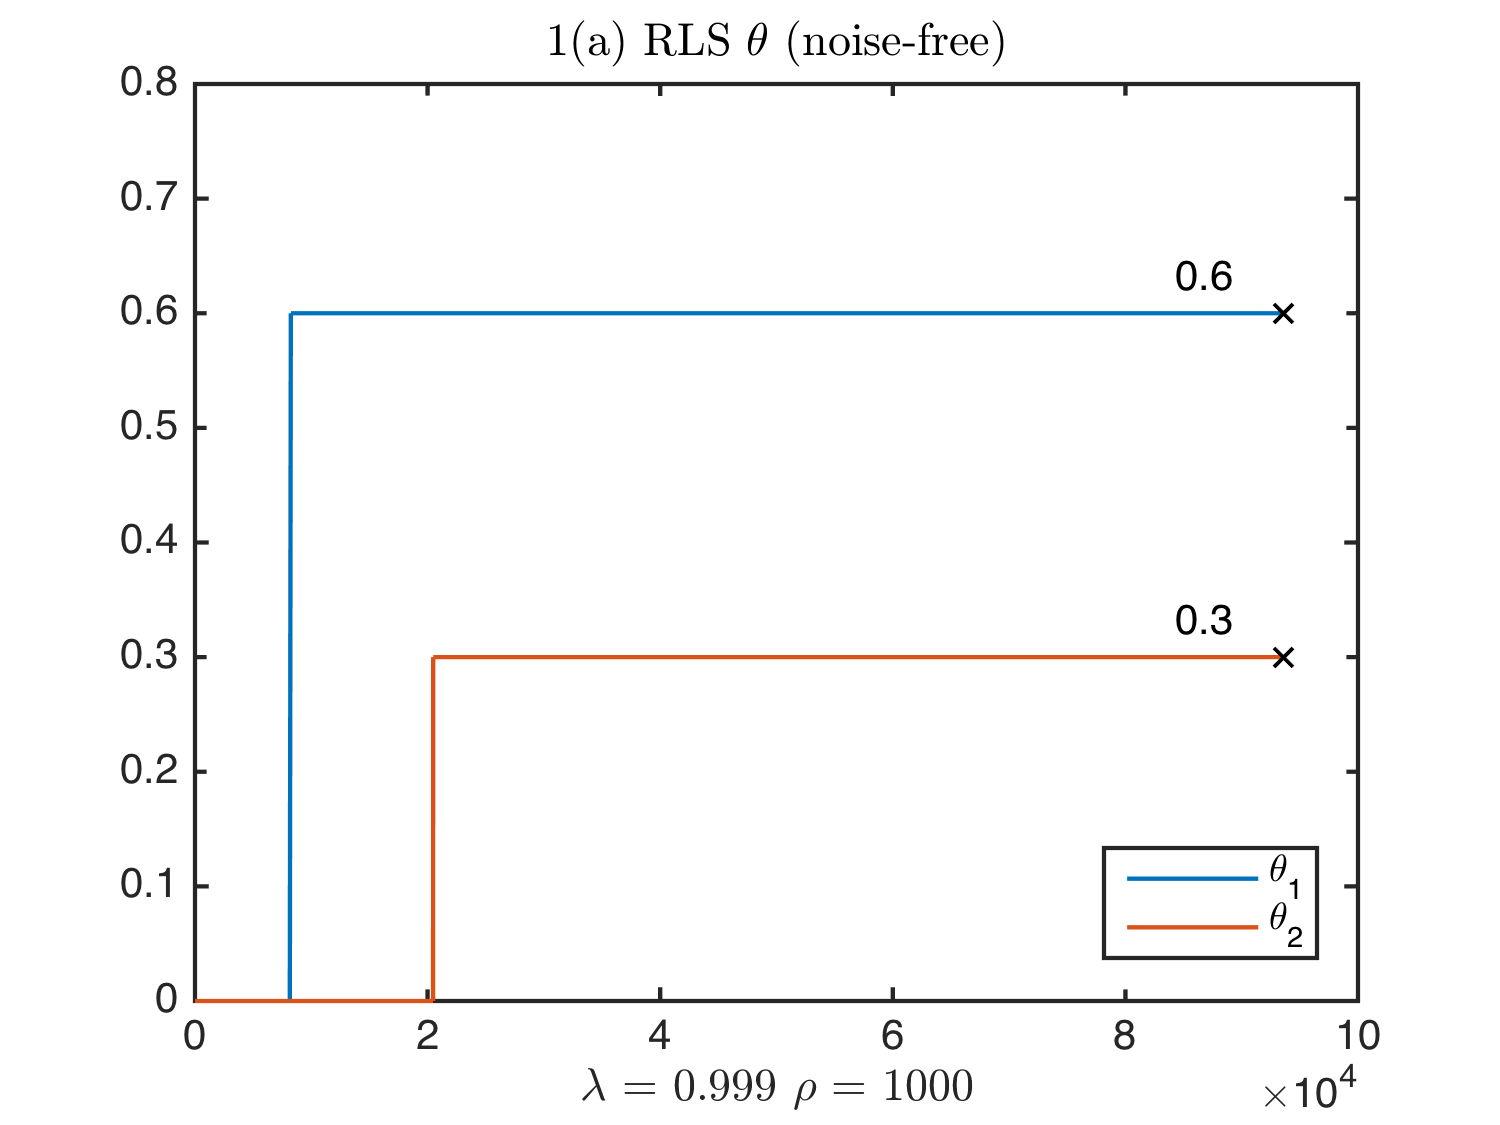
\includegraphics[width=2.5in]{a-rls-theta-noise-free}
\caption{RLS $\theta$ trends}
\label{a-rls-theta-noise-free}
\end{minipage}
\begin{minipage}[t]{0.33\linewidth}
\centering
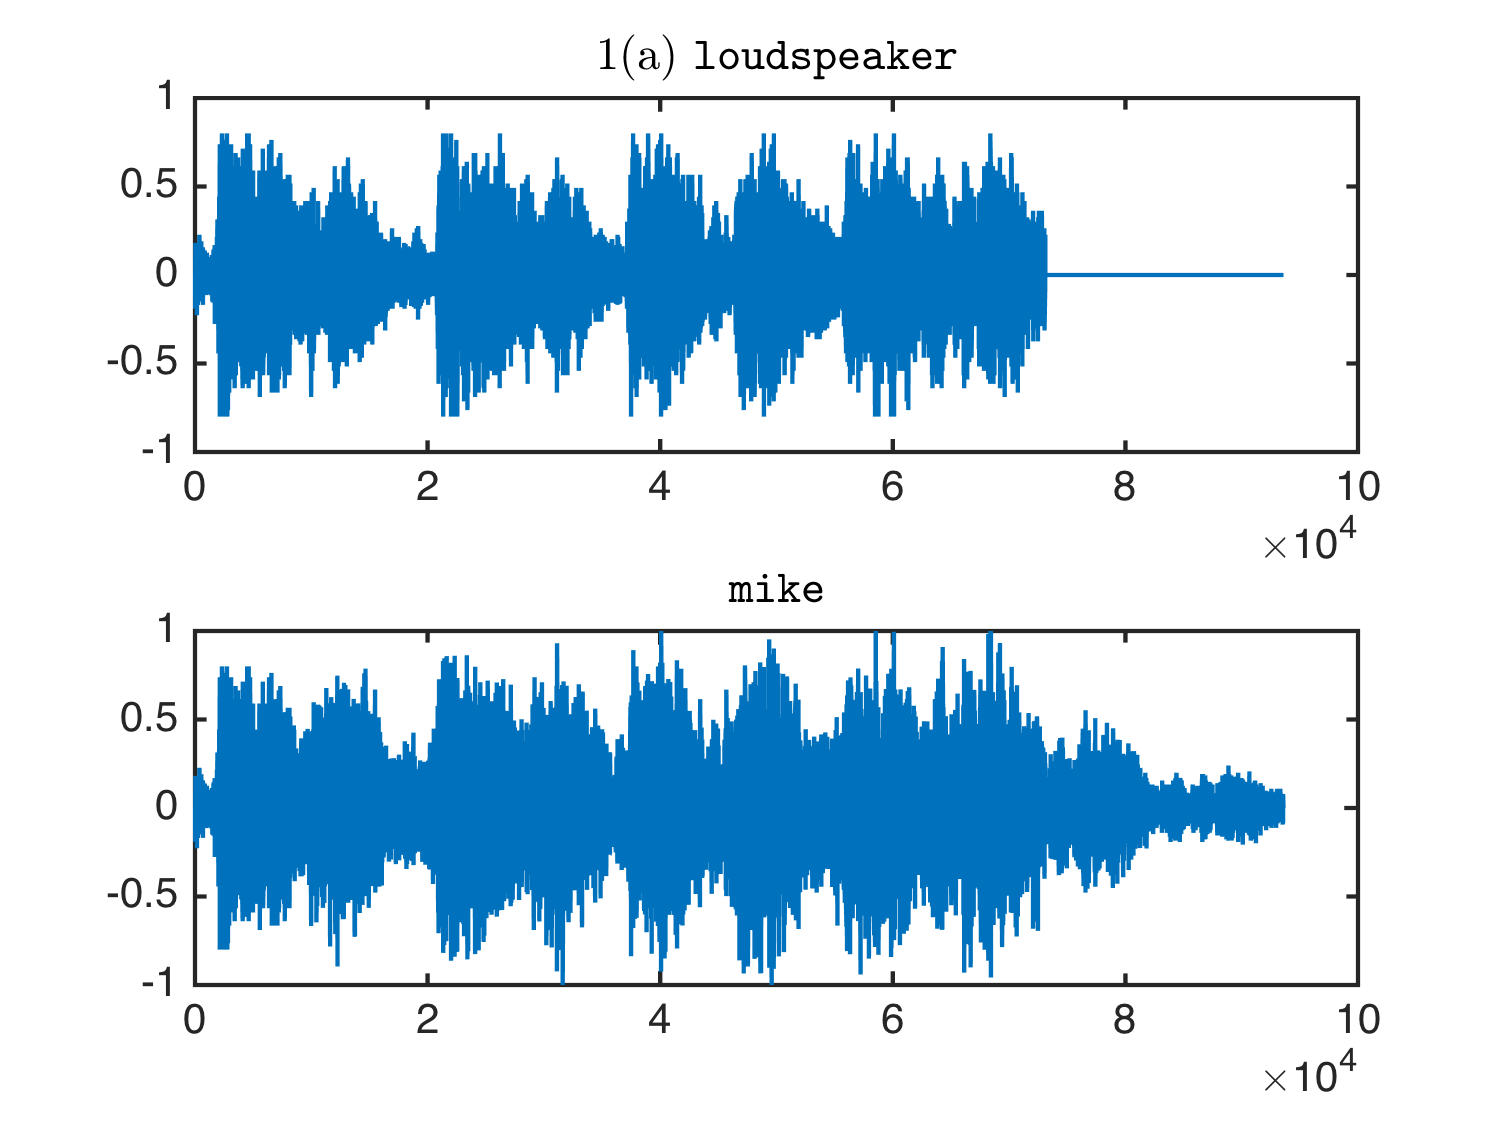
\includegraphics[width=2.5in]{a-rls-input-noise-free}
\caption{inputs}
\end{minipage}
\begin{minipage}[t]{0.33\linewidth}
\centering
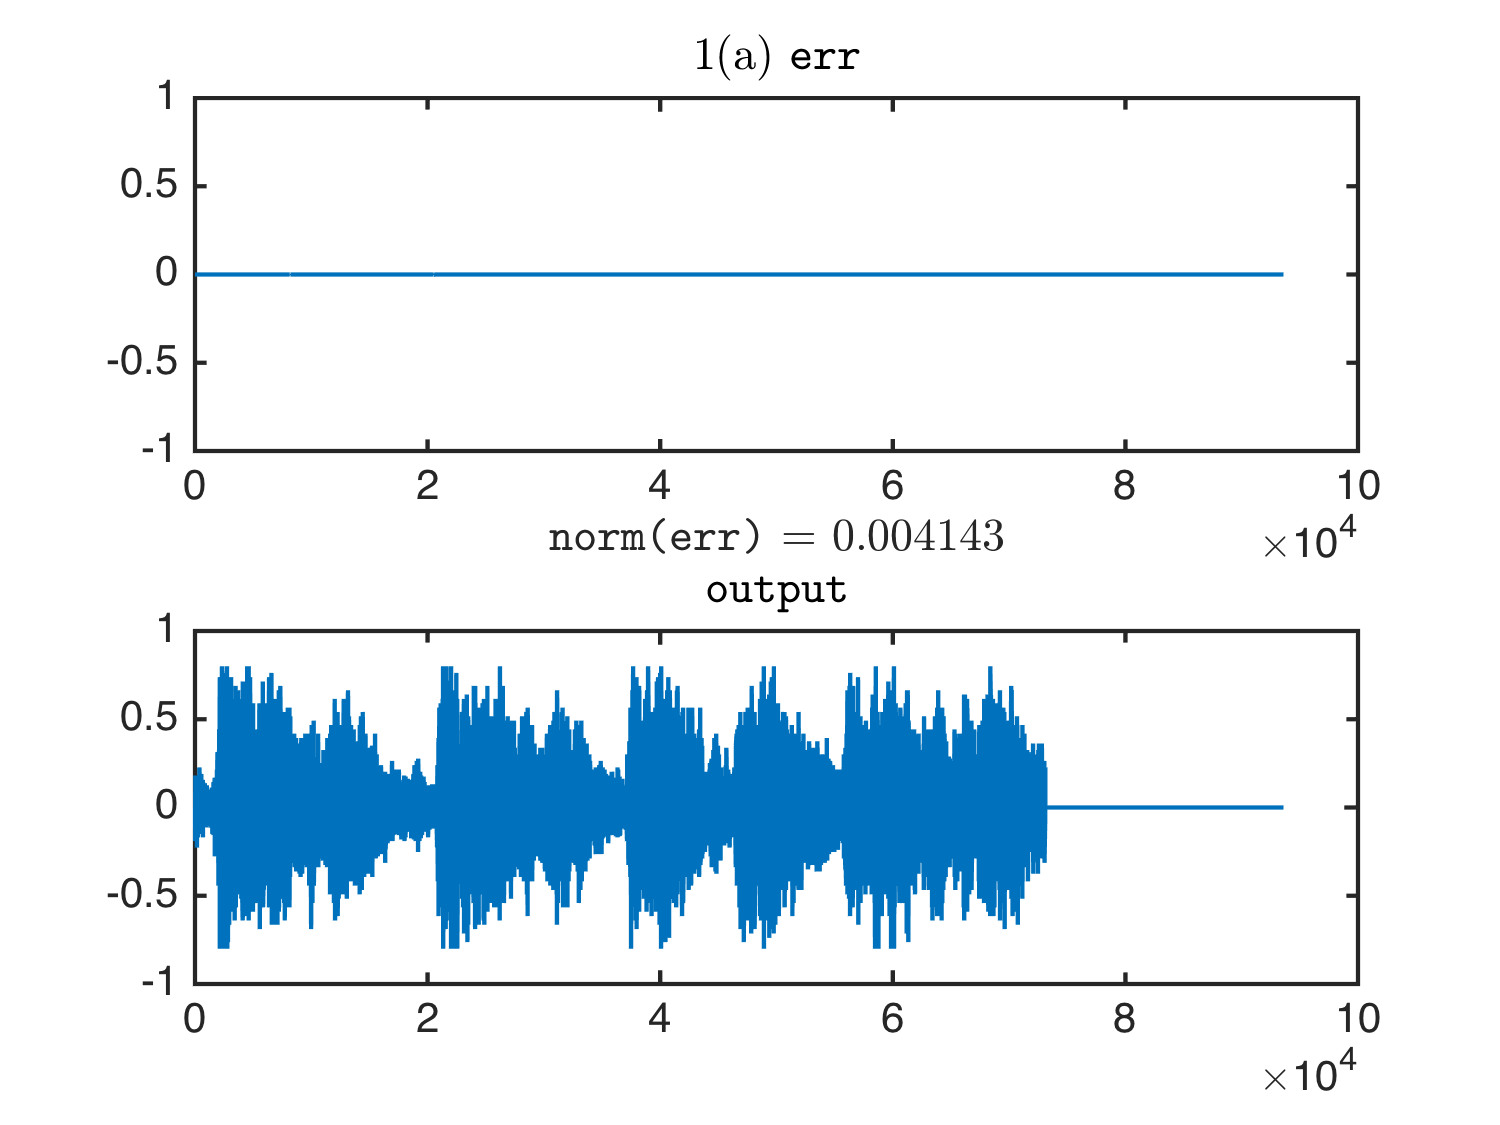
\includegraphics[width=2.5in]{a-rls-output-noise-free}
\caption{output and comparison}
\label{a-rls-output-noise-free}
\end{minipage}
\end{figure}

In Fig. \ref{a-rls-theta-noise-free}, $\theta_1$ and $\theta_2$ eventually converge to 0.6 and 0.3. In Fig. \ref{a-rls-output-noise-free}, echoes are successfully suppressed and \texttt{err} is negligible comparing with \texttt{mike1}.

\begin{lstlisting}[language={}]
Elapsed time is 1.341335 seconds.
lambda = 0.999000
rho = 1000.000000
norm(err) = 0.004143
\end{lstlisting}

\textbf{Improper choice of $\lambda$ and $\rho$}\\

In Fig. \ref{small-lambda}, smaller $\lambda = 0.998$ leads to severe overshoot. If we reduce $\lambda$ further, $\theta$ will become zero.\\

In Fig. \ref{small-rho}, smaller $\rho = 0.001$ results in longer transition time.

\begin{figure}[H]
\begin{minipage}[t]{0.5\linewidth}
\centering
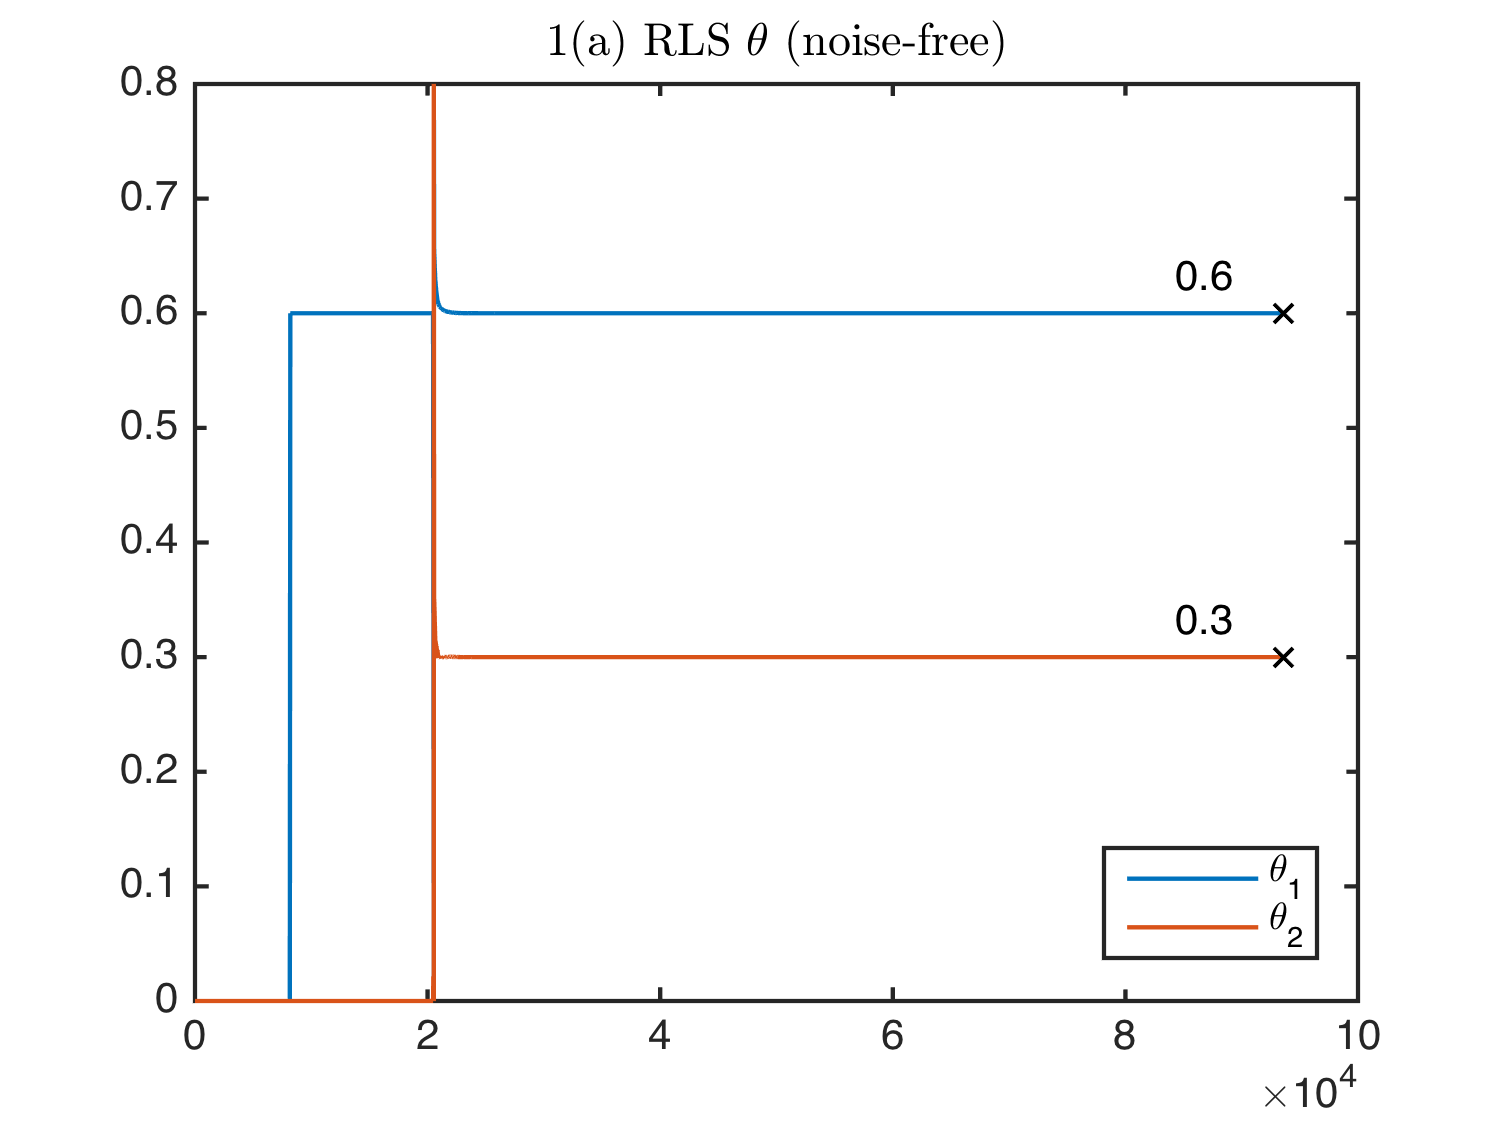
\includegraphics[width=3.3in]{small-lambda}
\caption{small $\lambda$}
\label{small-lambda}
\end{minipage}
\begin{minipage}[t]{0.5\linewidth}
\centering
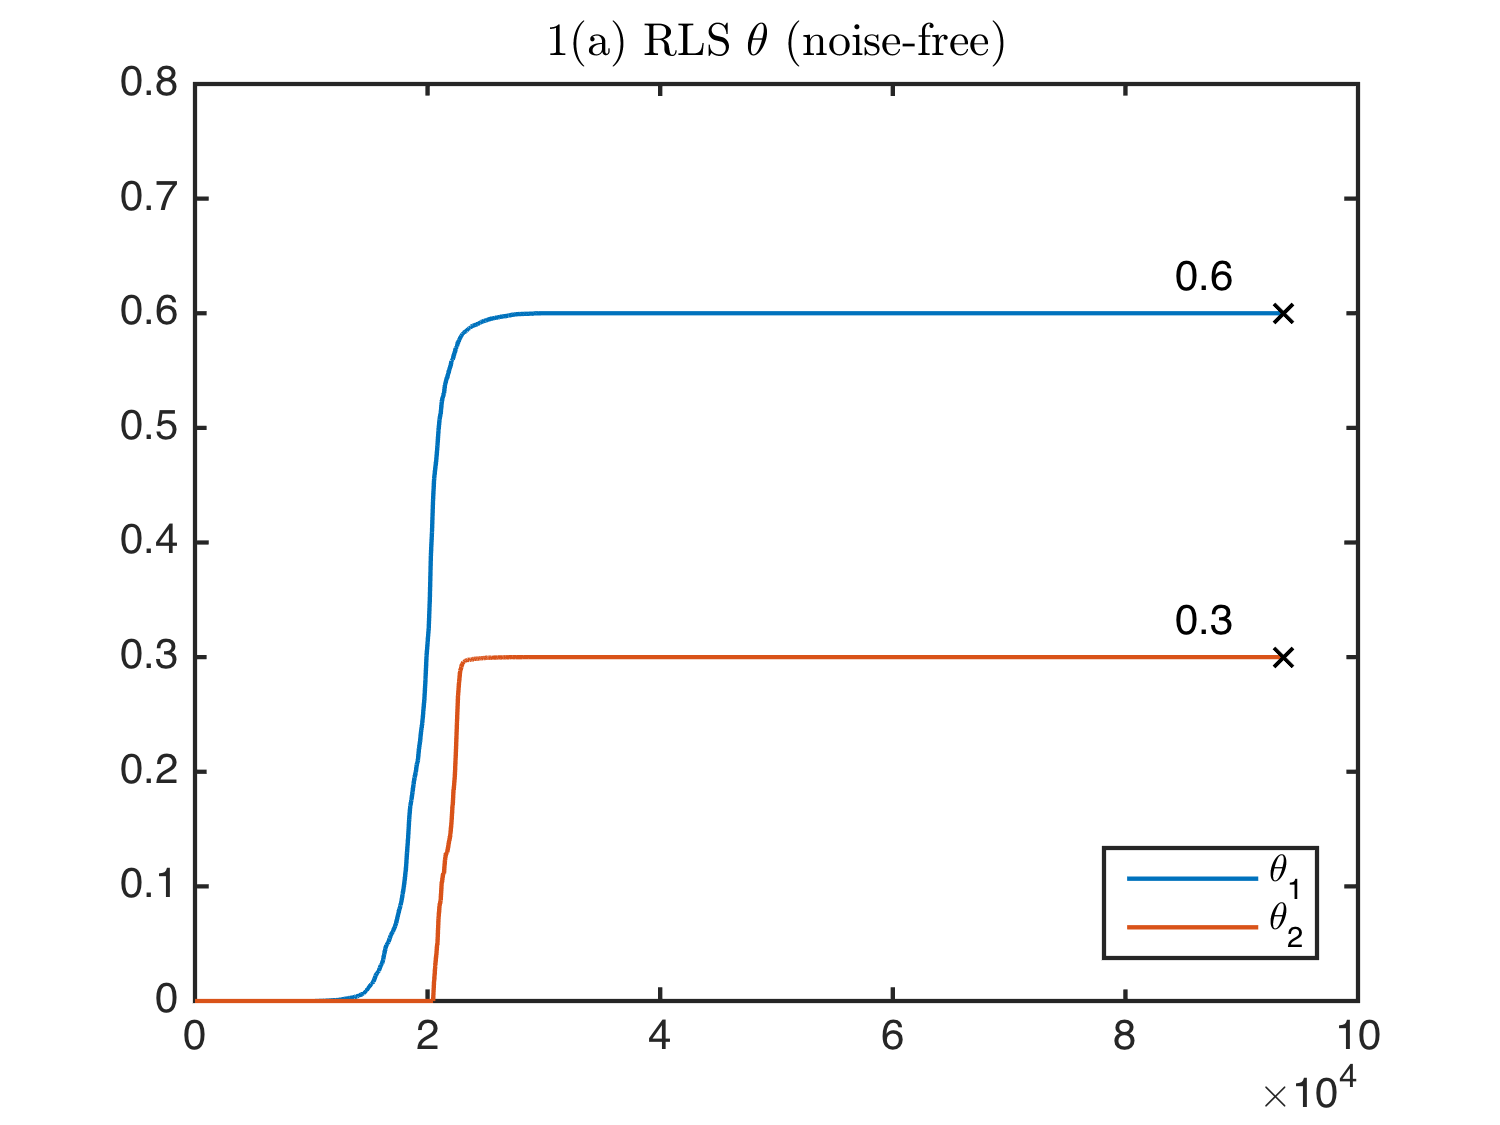
\includegraphics[width=3.3in]{small-rho}
\caption{small $\rho$}
\label{small-rho}
\end{minipage}
\end{figure}

%--------------------------------------------

\subsubsection*{Noisy environment}

By trial and error, we find when $\lambda = 0.999$, $\rho = 0.1$, the RLS filter has best echo-cancellation performance.
\begin{center}
\texttt{norm(err)} = 4.849423 $>$ 0.004143
\end{center}
\texttt{norm(err)} increases due to the interference of the background noise.

\begin{figure}[H]
\begin{minipage}[t]{0.33\linewidth}
\centering
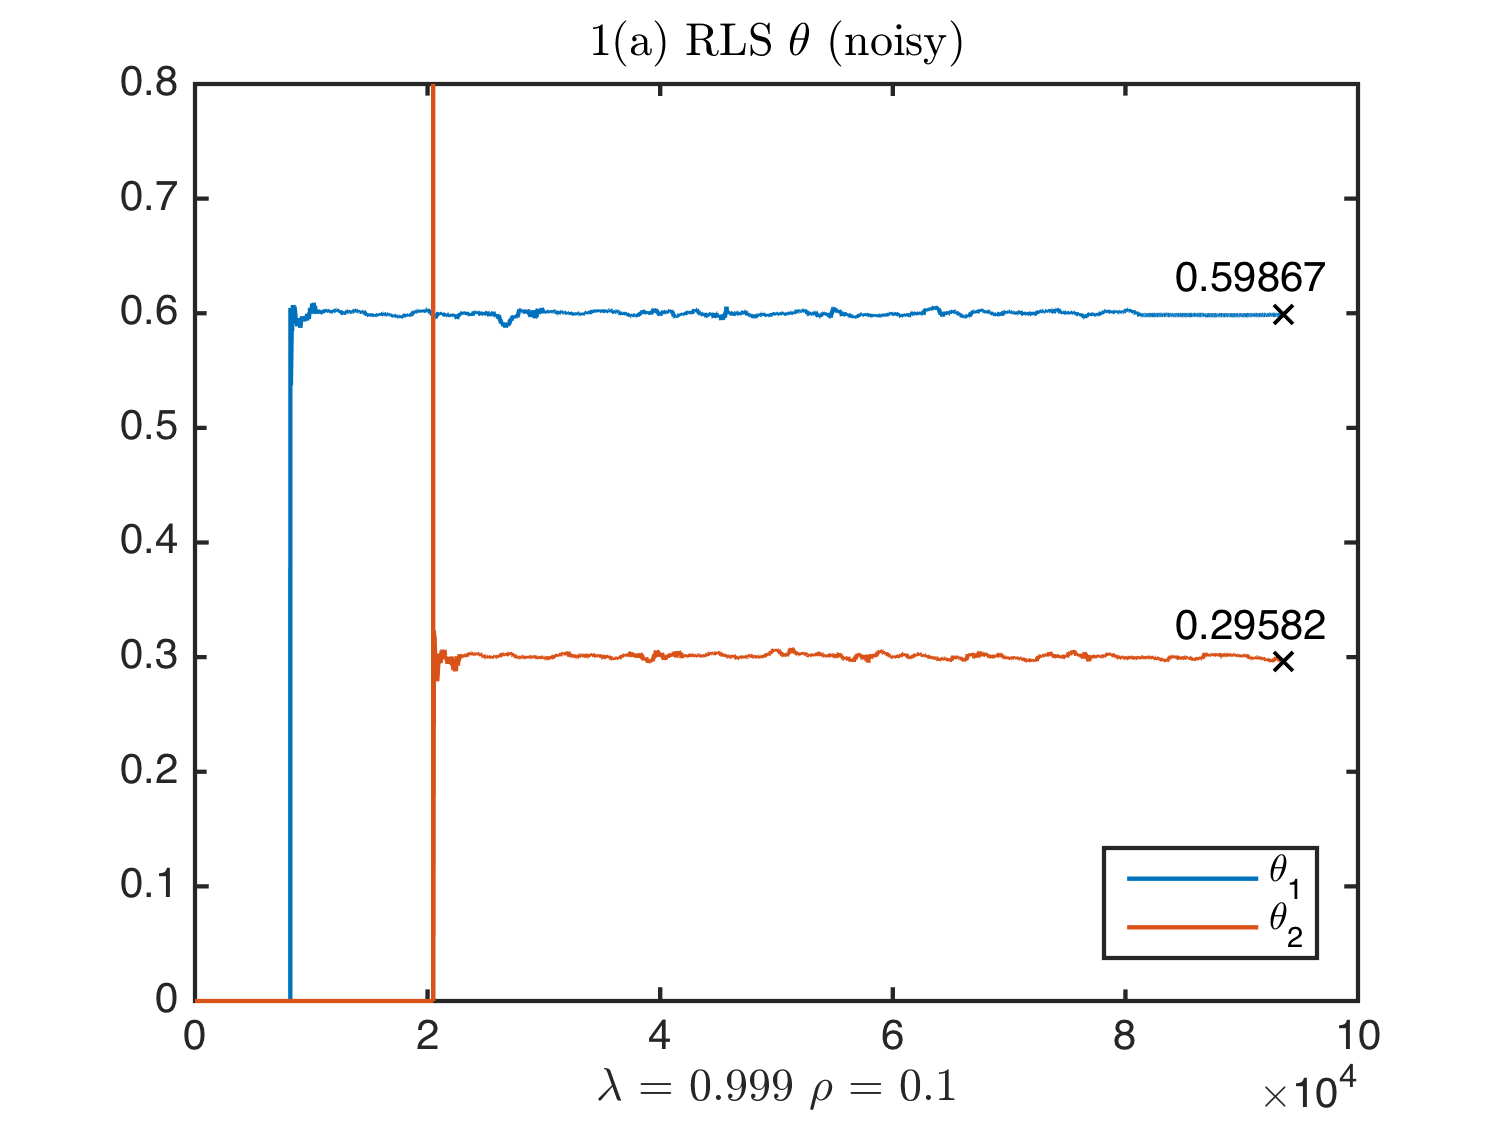
\includegraphics[width=2.5in]{a-rls-theta-noisy}
\caption{RLS $\theta$ trends}
\label{a-rls-theta-noisy}
\end{minipage}
\begin{minipage}[t]{0.33\linewidth}
\centering
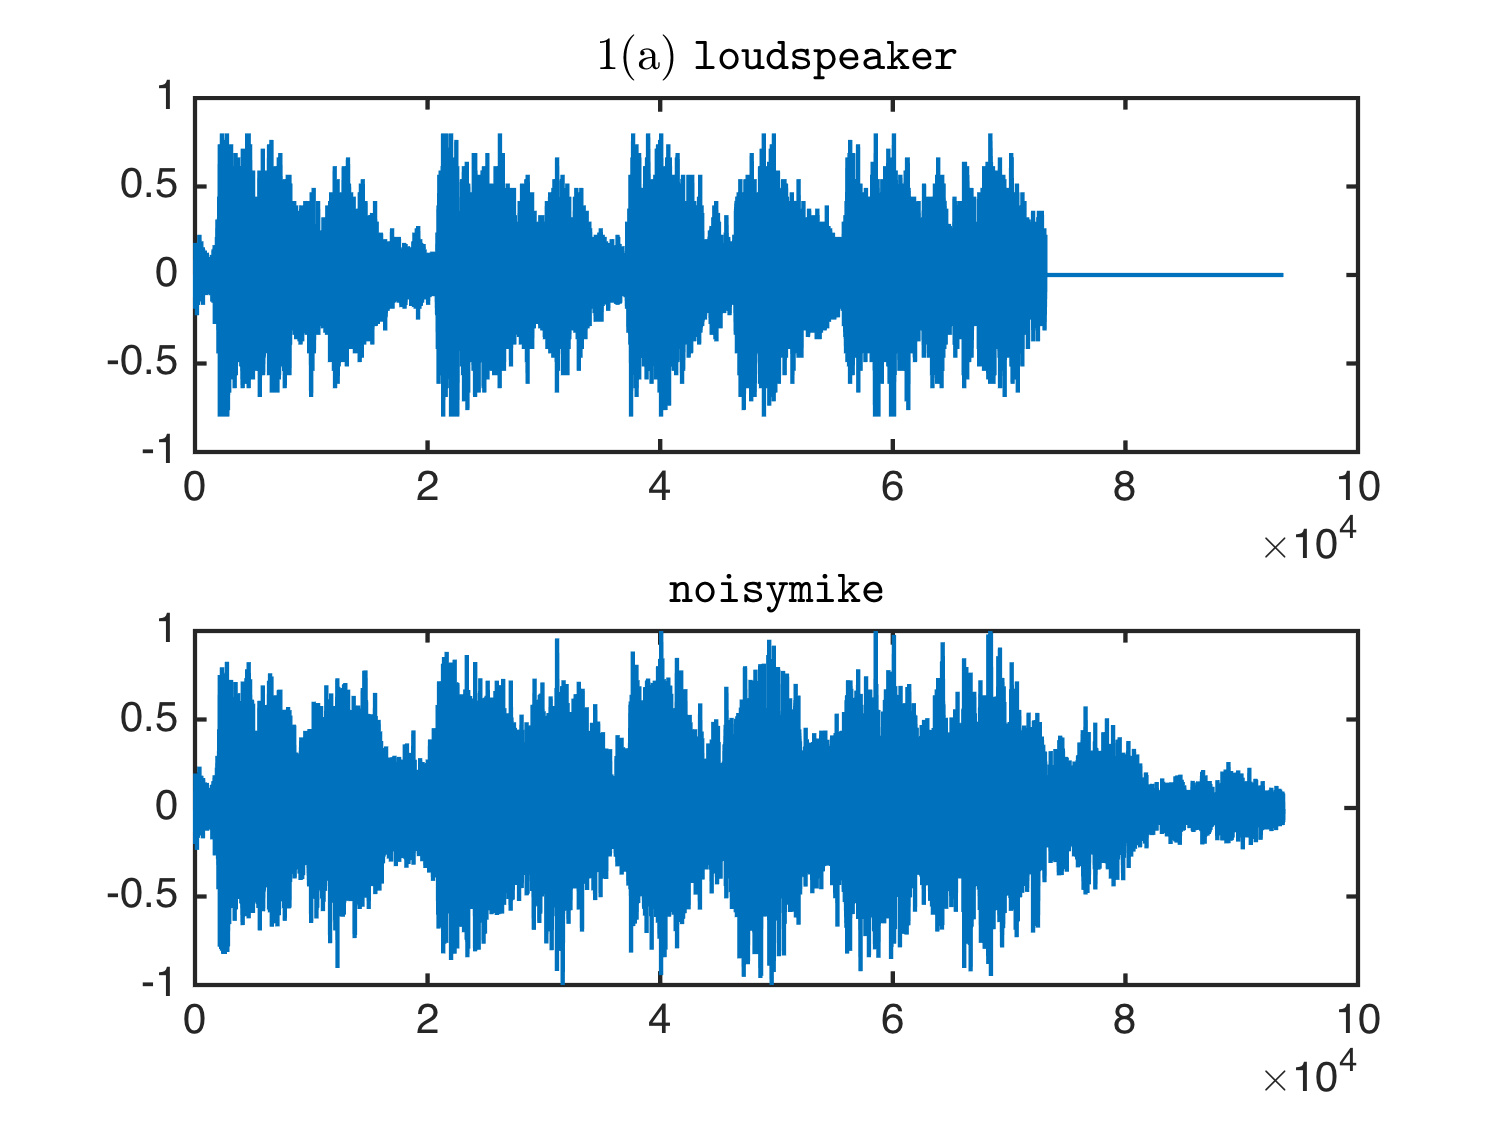
\includegraphics[width=2.5in]{a-rls-input-noisy}
\caption{inputs}
\end{minipage}
\begin{minipage}[t]{0.33\linewidth}
\centering
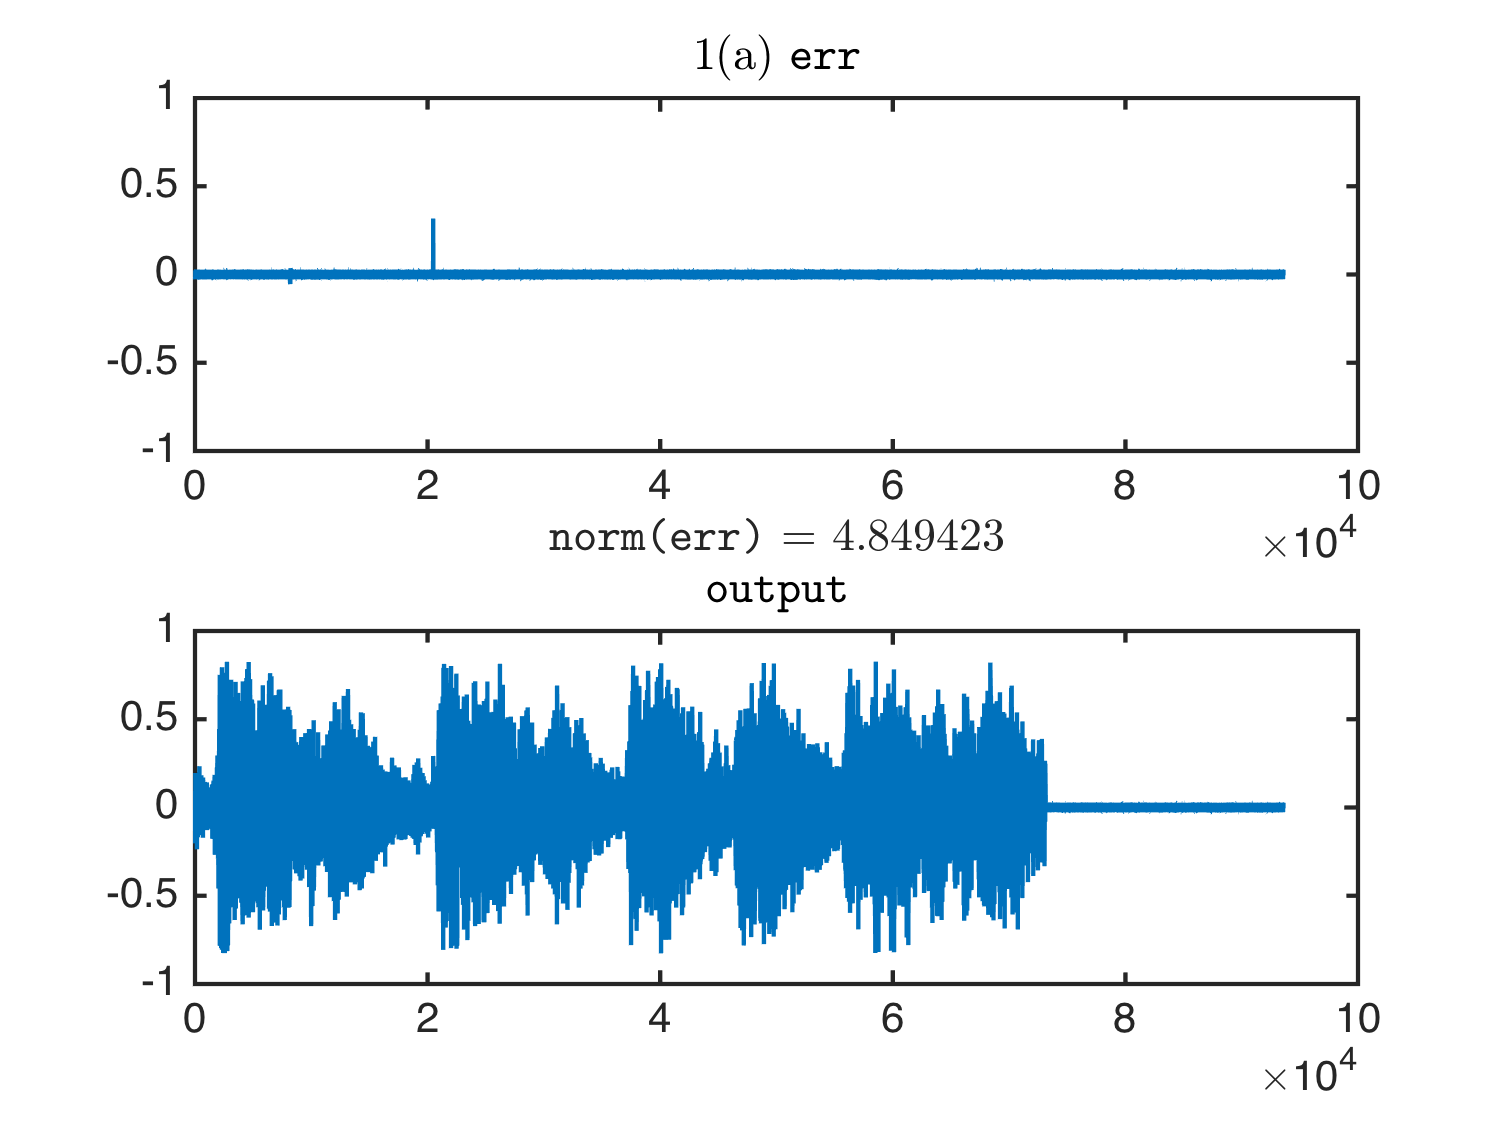
\includegraphics[width=2.5in]{a-rls-output-noisy}
\caption{output and comparison}
\label{a-rls-output-noisy}
\end{minipage}
\end{figure}

In Fig. \ref{a-rls-theta-noisy}, $\theta_1$ and $\theta_2$ eventually converge to 0.599 and 0.296. In Fig. \ref{a-rls-output-noisy}, echoes are successfully suppressed and \texttt{err} is negligible comparing with \texttt{noisymike1}.

%--------------------------------------------
%--------------------------------------------

\subsection*{LMS}

\subsubsection*{Noise-free environment}

By trial and error, we find when \texttt{step\_size} = 2$\mu$ = 10, the LMS filter has best echo-cancellation performance.
\begin{center}
\texttt{norm(err)} = 0.158492
\end{center}

\begin{figure}[H]
\begin{minipage}[t]{0.33\linewidth}
\centering
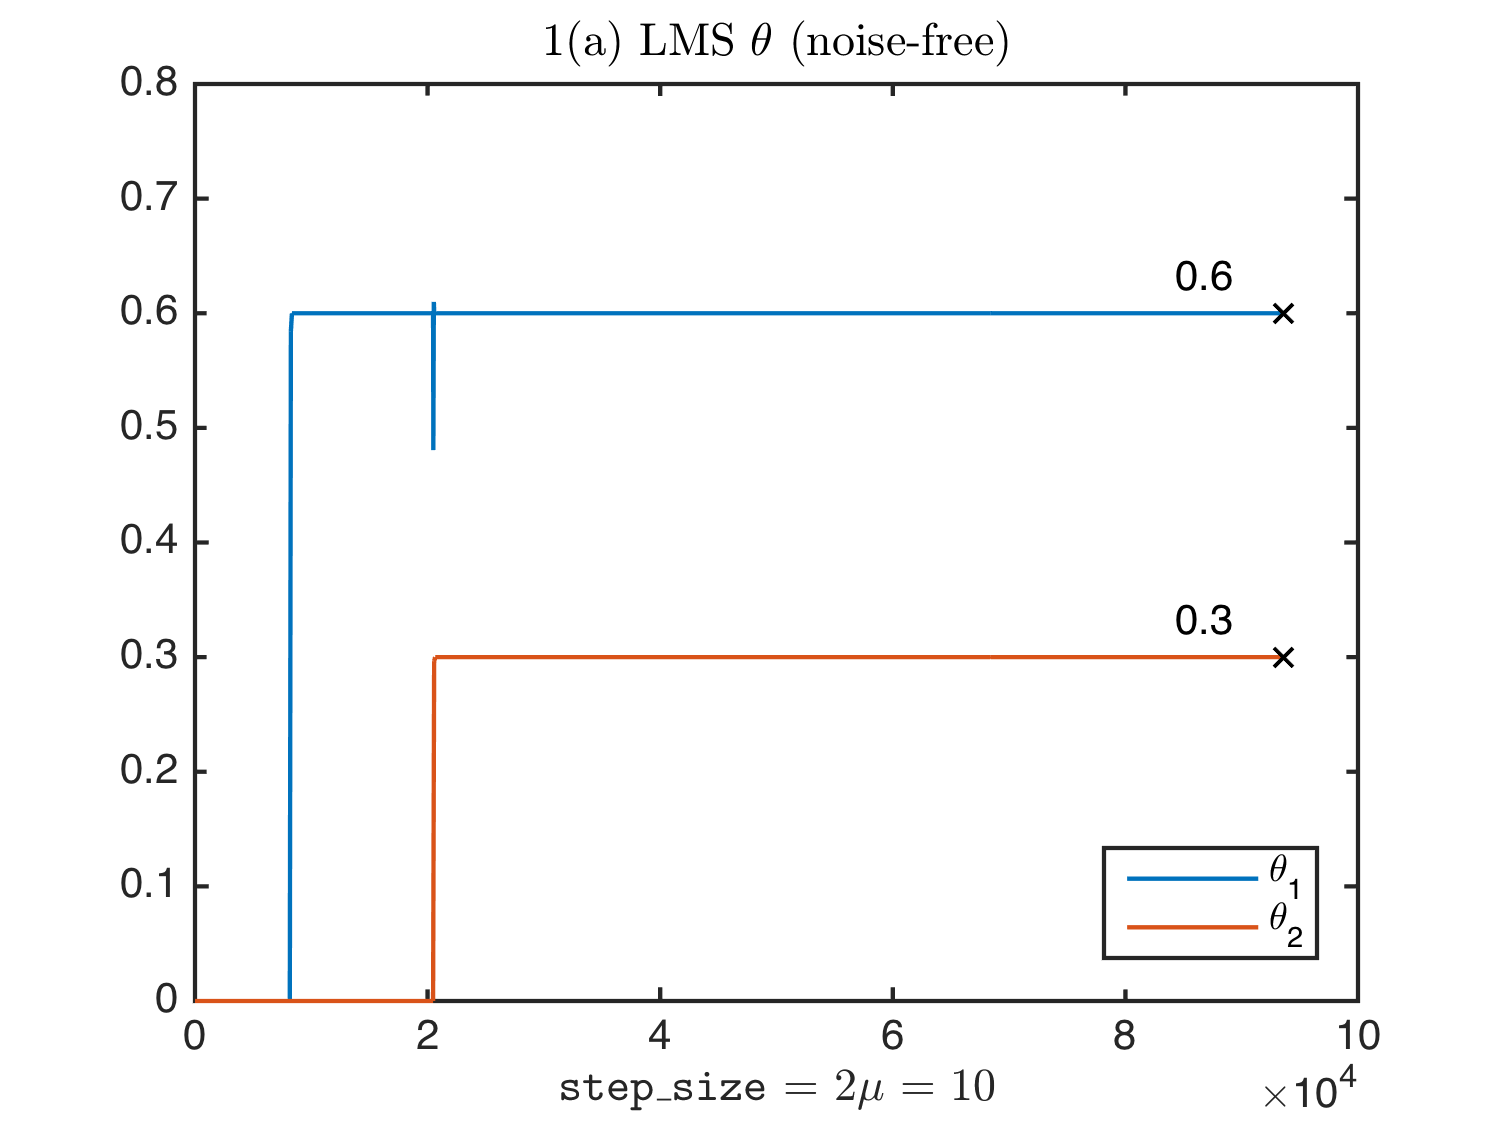
\includegraphics[width=2.5in]{a-lms-theta-noise-free}
\caption{LMS $\theta$ trends}
\label{a-lms-theta-noise-free}
\end{minipage}
\begin{minipage}[t]{0.33\linewidth}
\centering
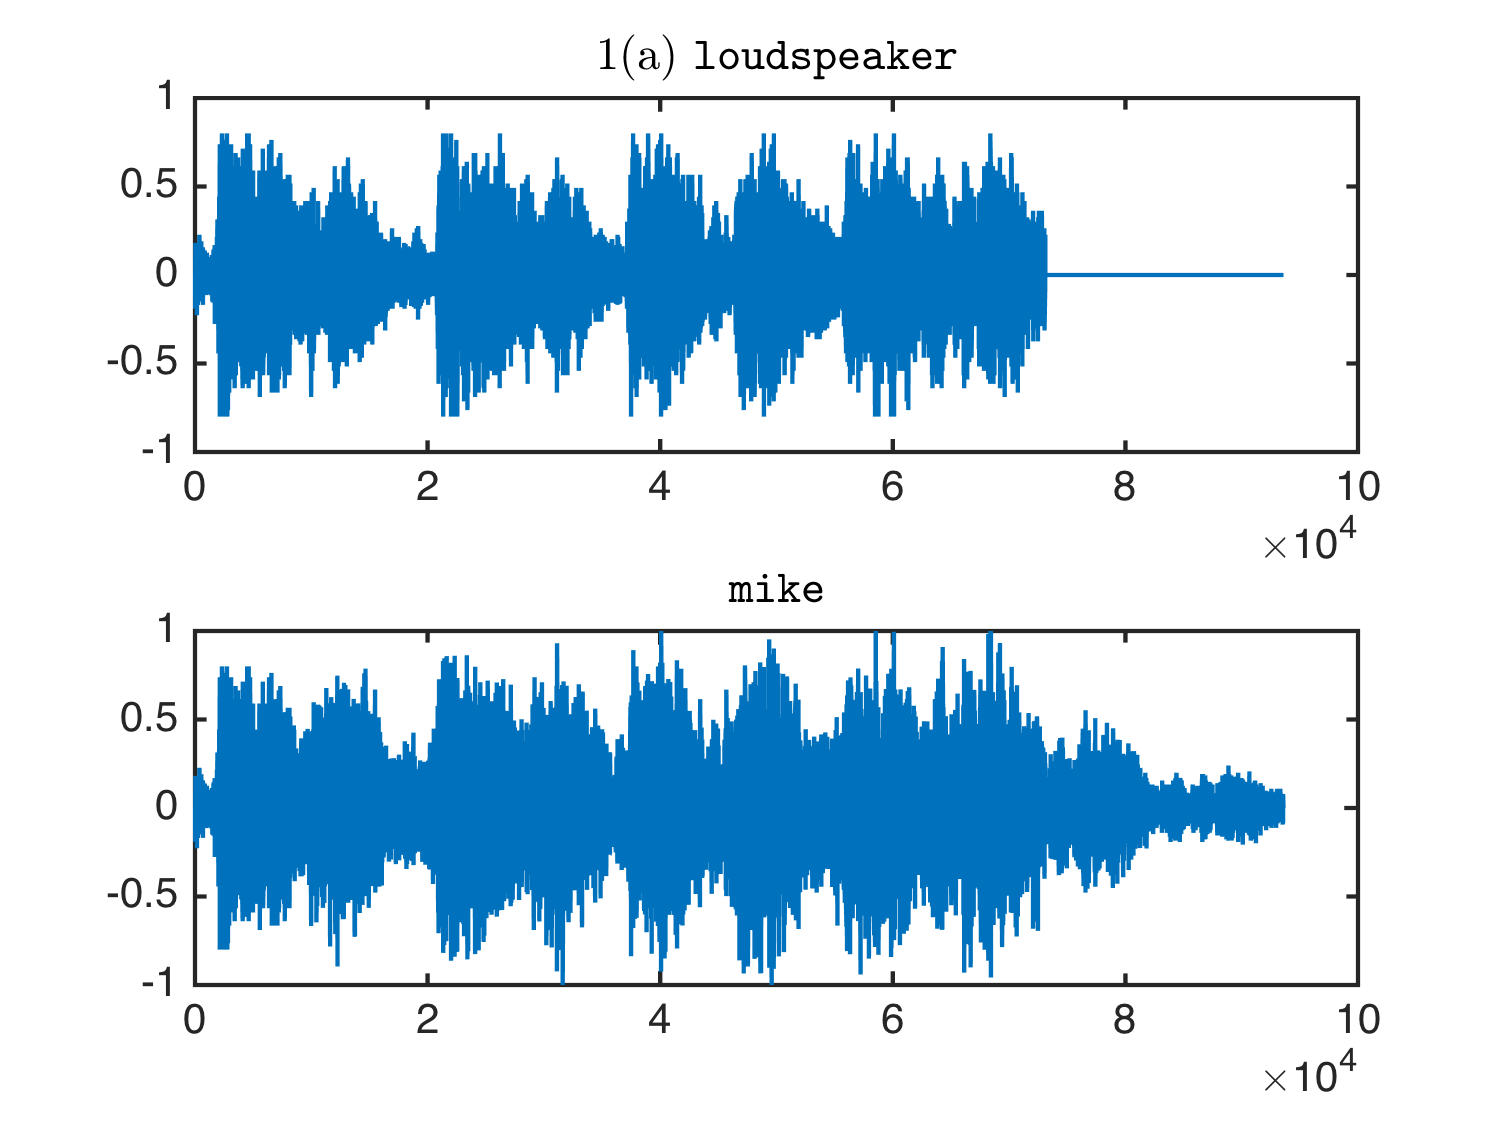
\includegraphics[width=2.5in]{a-lms-input-noise-free}
\caption{inputs}
\end{minipage}
\begin{minipage}[t]{0.33\linewidth}
\centering
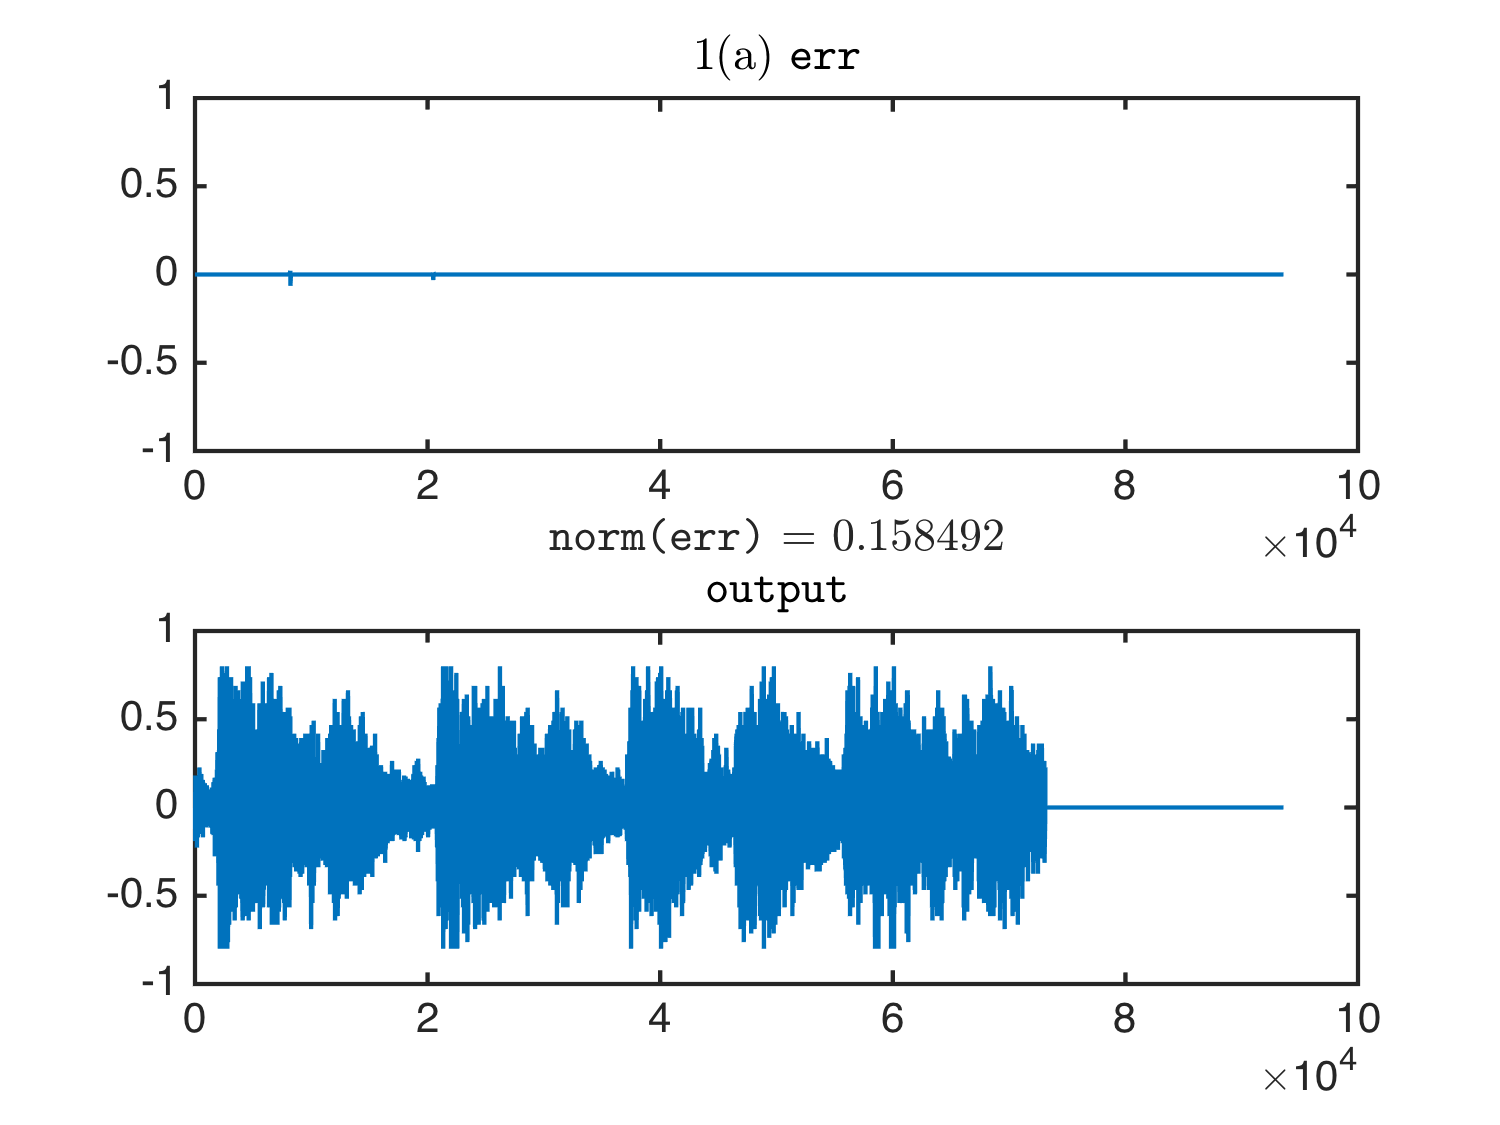
\includegraphics[width=2.5in]{a-lms-output-noise-free}
\caption{output and comparison}
\label{a-lms-output-noise-free}
\end{minipage}
\end{figure}

In Fig. \ref{a-lms-theta-noise-free}, $\theta_1$ and $\theta_2$ eventually converge to 0.6 and 0.3. In Fig. \ref{a-lms-output-noise-free}, echoes are successfully suppressed and \texttt{err} is negligible comparing with \texttt{mike1}.

\begin{lstlisting}[language={}]
Elapsed time is 0.603833 seconds.
step_size = 10.000000
norm(err) = 0.158492
\end{lstlisting}

\textbf{Improper choice of $\mu$}\\

In Fig. \ref{big-mu}, bigger \texttt{step\_size} = 2$\mu$ = 11 leads to instability. If we increase \texttt{step\_size} further, the LMS filter will diverge and become unstable.\\

In Fig. \ref{small-mu}, smaller \texttt{step\_size} = 2$\mu$ = 0.001 results in longer transition time.

\begin{figure}[H]
\begin{minipage}[t]{0.5\linewidth}
\centering
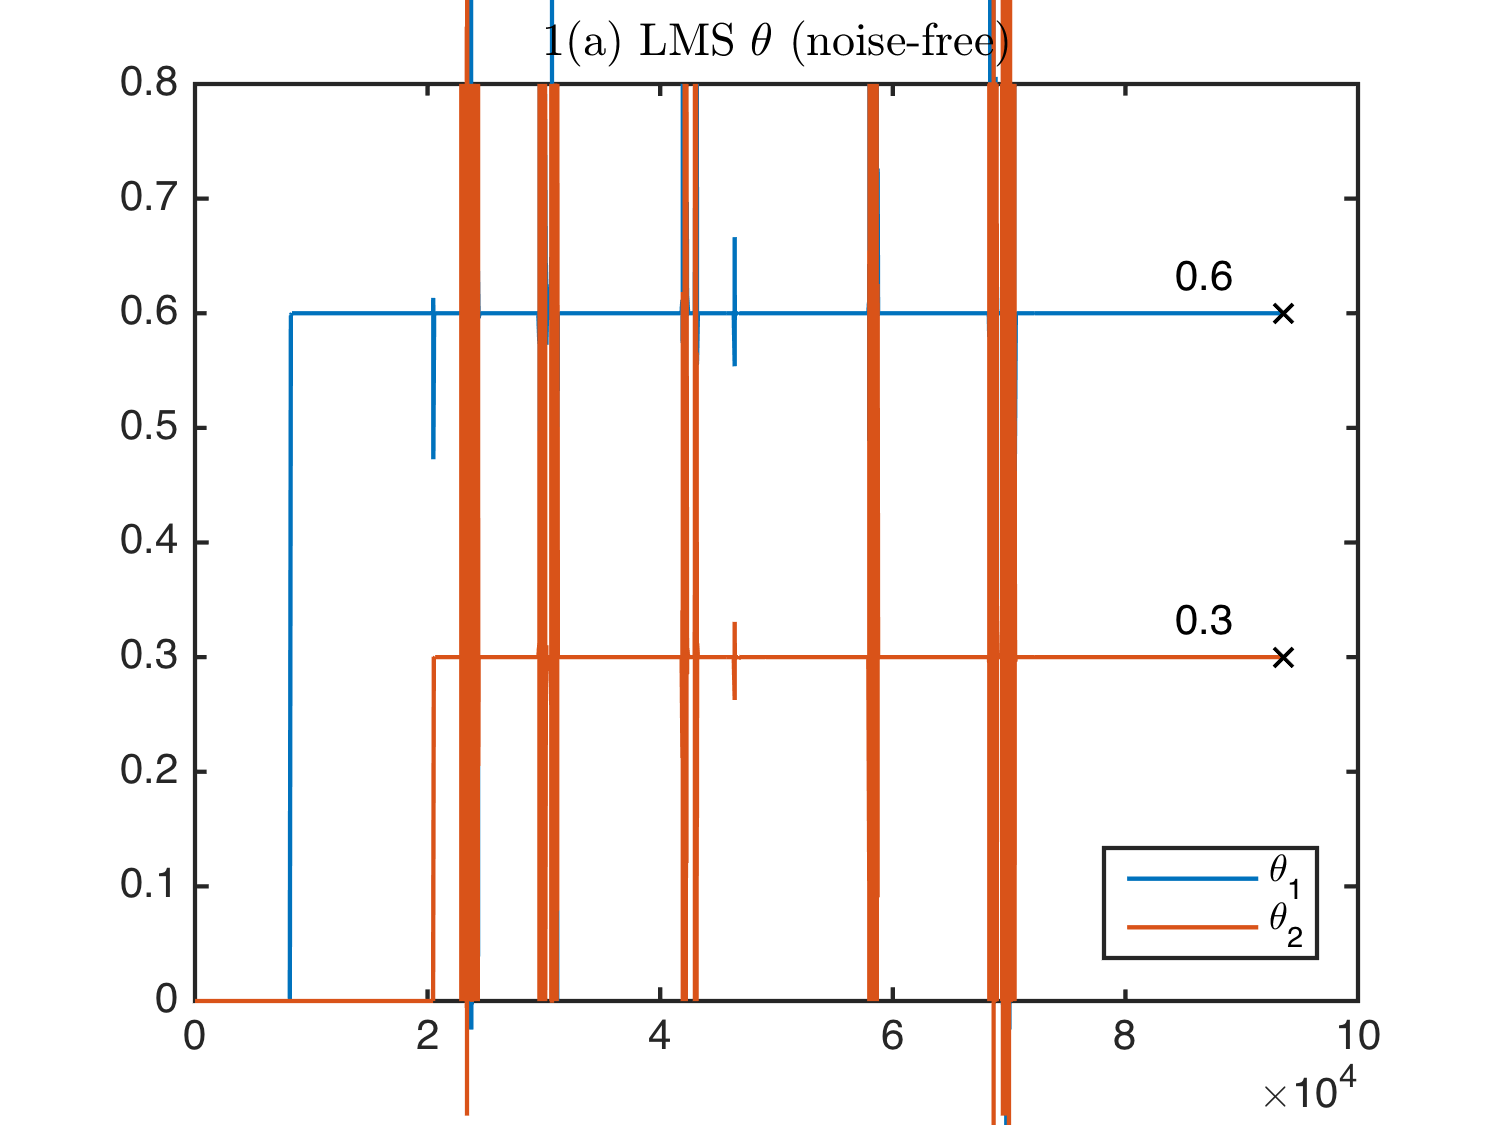
\includegraphics[width=3.3in]{big-mu}
\caption{big $\mu$}
\label{big-mu}
\end{minipage}
\begin{minipage}[t]{0.5\linewidth}
\centering
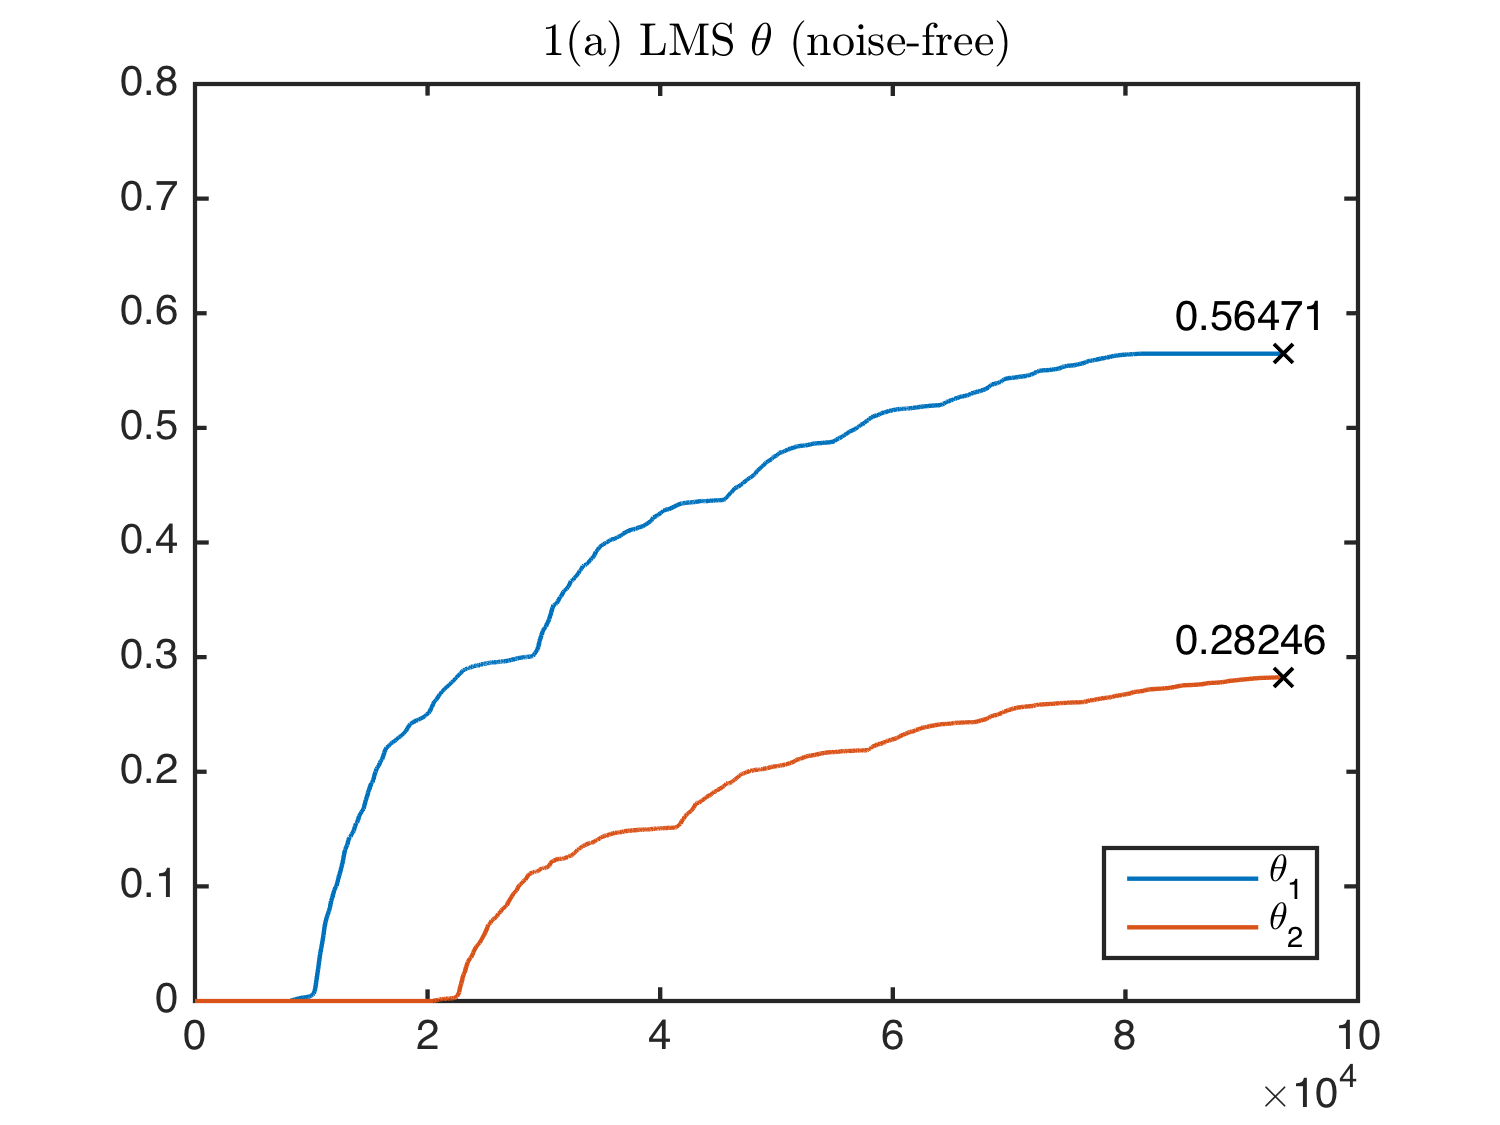
\includegraphics[width=3.3in]{small-mu}
\caption{small $\mu$}
\label{small-mu}
\end{minipage}
\end{figure}

%--------------------------------------------

\subsubsection*{Noisy environment}

By trial and error, we find when \texttt{step\_size} = 2$\mu$ = 0.5, the LMS filter has best echo-cancellation performance.
\begin{center}
\texttt{norm(err)} = 4.919796 $>$ 0.158492
\end{center}
\texttt{norm(err)} increases due to the interference of the background noise.

\begin{figure}[H]
\begin{minipage}[t]{0.33\linewidth}
\centering
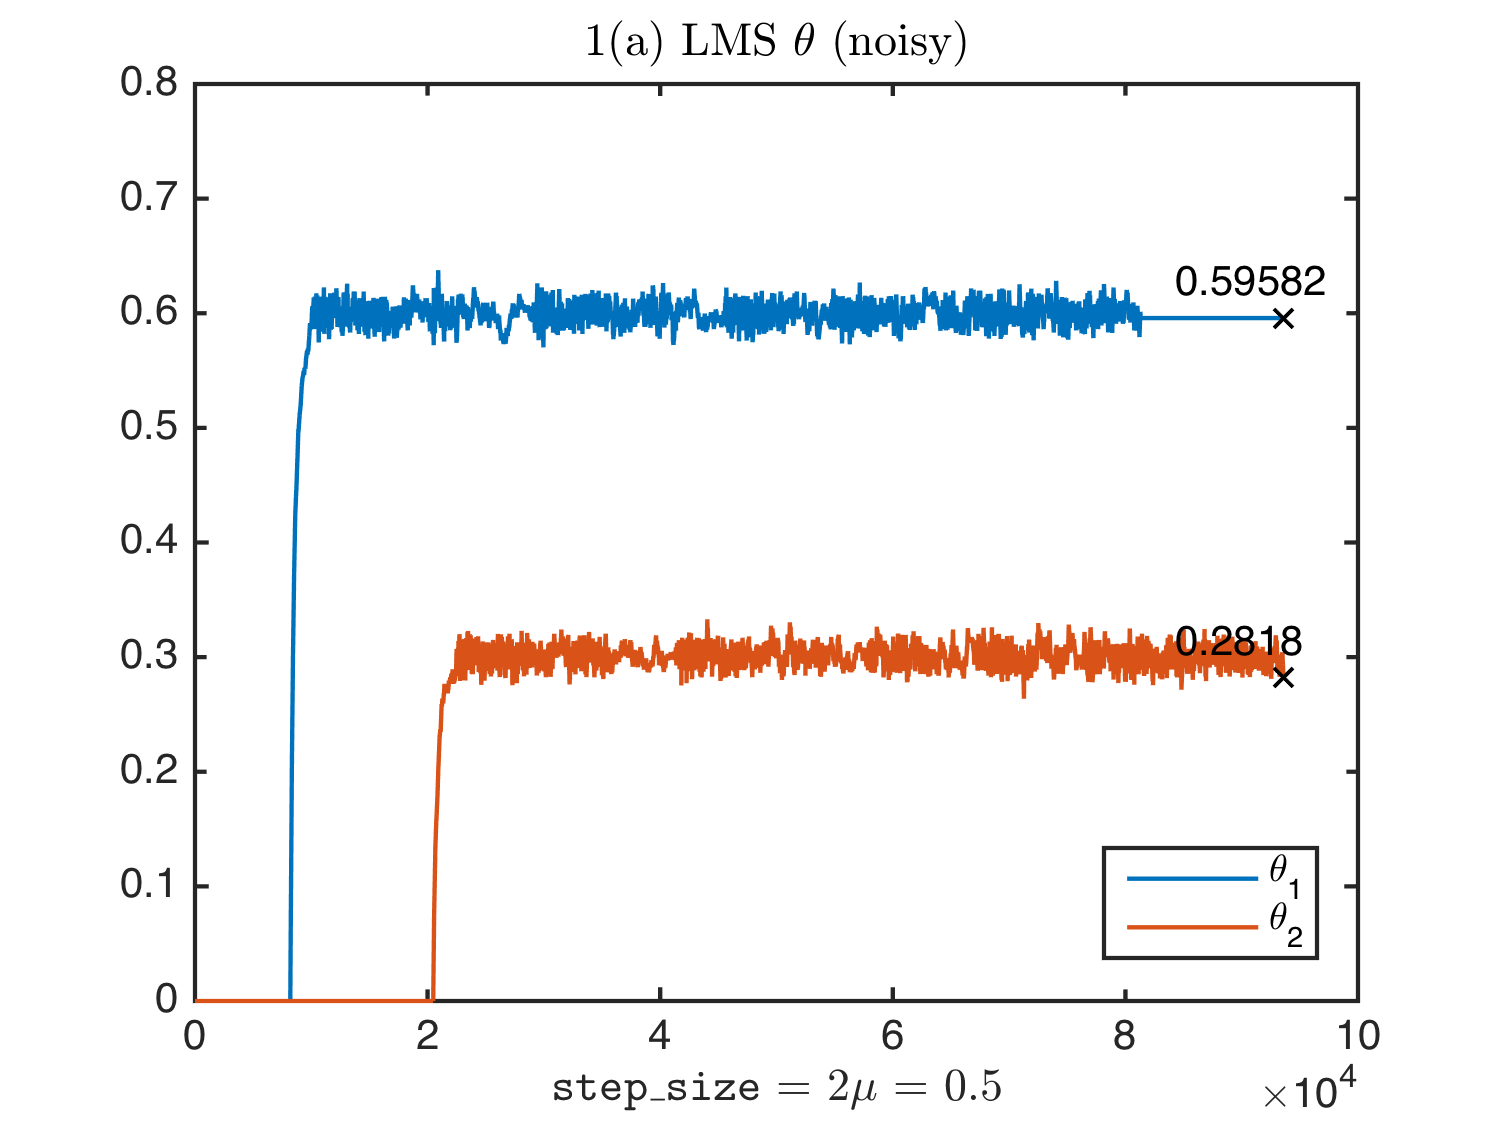
\includegraphics[width=2.5in]{a-lms-theta-noisy}
\caption{LMS $\theta$ trends}
\label{a-lms-theta-noisy}
\end{minipage}
\begin{minipage}[t]{0.33\linewidth}
\centering
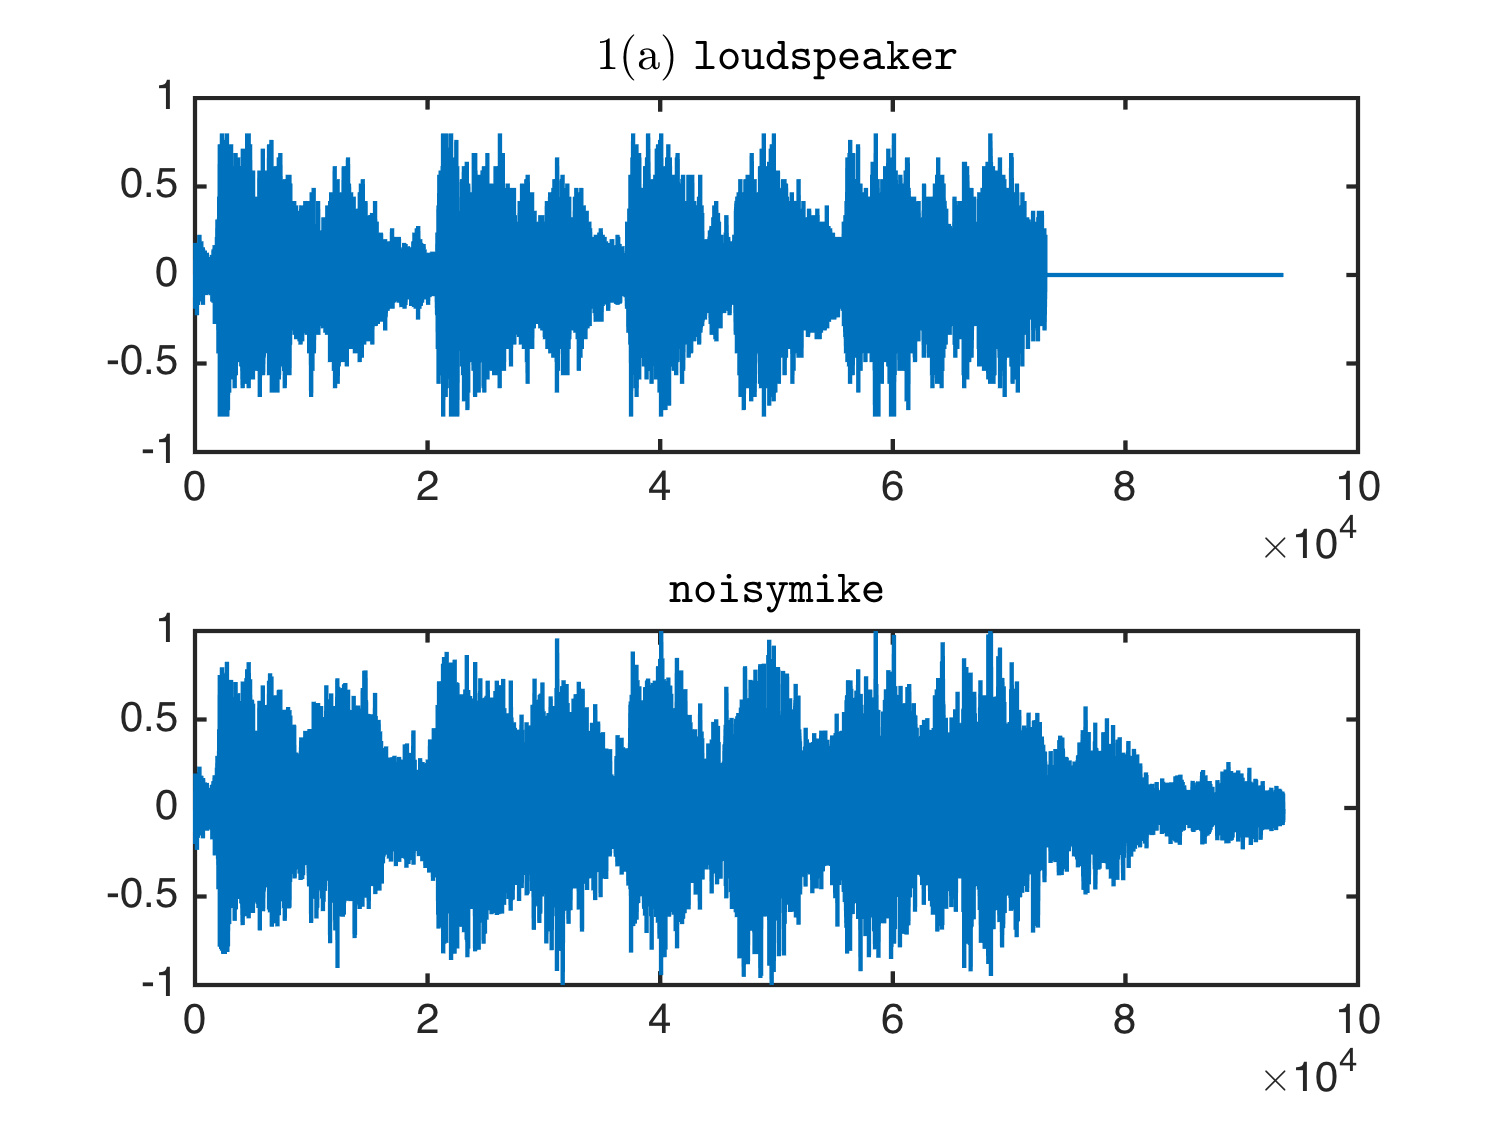
\includegraphics[width=2.5in]{a-lms-input-noisy}
\caption{inputs}
\end{minipage}
\begin{minipage}[t]{0.33\linewidth}
\centering
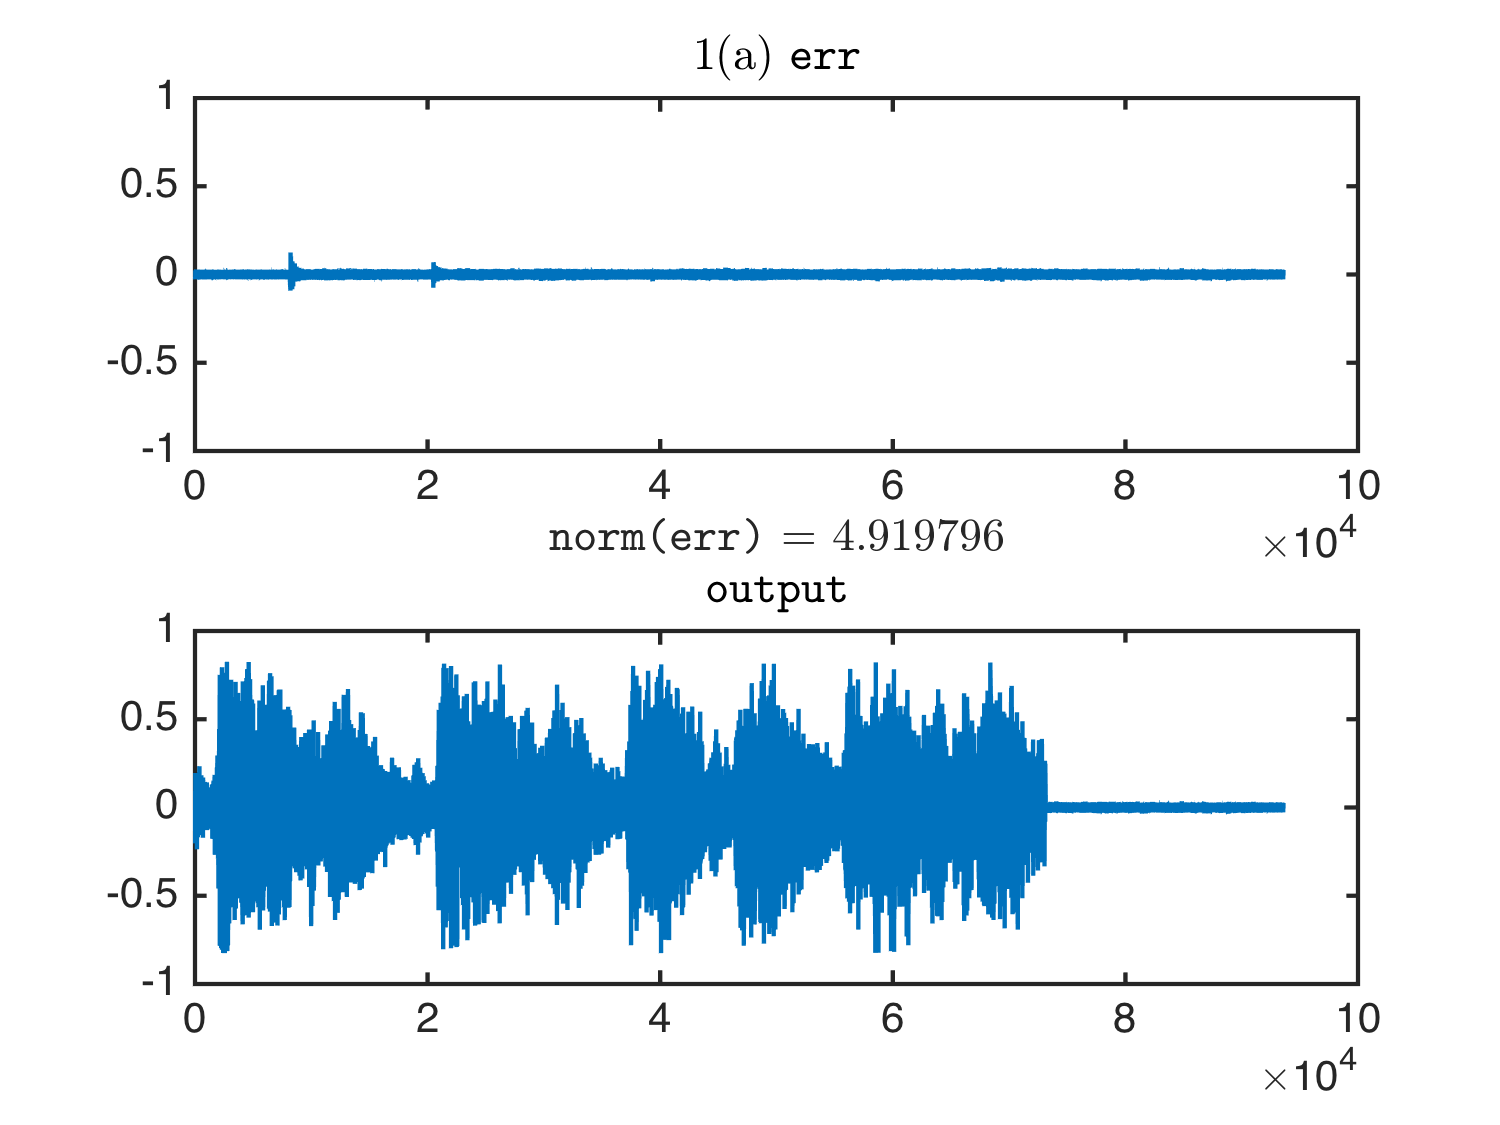
\includegraphics[width=2.5in]{a-lms-output-noisy}
\caption{output and comparison}
\label{a-lms-output-noisy}
\end{minipage}
\end{figure}

In Fig. \ref{a-lms-theta-noisy}, $\theta_1$ and $\theta_2$ eventually converge to 0.596 and 0.282. In Fig. \ref{a-lms-output-noisy}, echoes are successfully suppressed and \texttt{err} is negligible comparing with \texttt{noisymike1}.

%--------------------------------------------
%--------------------------------------------

\subsection*{RLS \& LMS comparison}
$\theta_1$ and $\theta_2$ in both RLS and LMS converge to 0.3 and 0.6 rapidly. However, when the second echo arrives (at 2.5 s), $\theta_1$ in LMS has an abnormal spike (shown in Fig. \ref{a-lms-theta-noise-free}). Considering the echo amplitudes are constant, RLS is expected to perform better than LMS. In fact, \texttt{norm(err)} of RLS is smaller than LMS (0.004143 vs 0.158492).\\

We use \texttt{tic} and \texttt{toc} in MATLAB to measure time to run RLS or LMS algorithm. RLS is more time-consuming than LMS.
\begin{equation*}
\frac{\text{RLS}}{\text{LMS}} = \frac{1.341335\text{ seconds}}{0.603833\text{ seconds}} = 2.22
\end{equation*}

%----------------------------------------------------------------------------------------
%	Task 1 (b)
%----------------------------------------------------------------------------------------

\section*{Task 1 (b) time-varying echo amplitude}

\subsection*{RLS}

\subsubsection*{Noise-free environment}

By trial and error, we find when $\lambda = 0.999$, $\rho = 1000$, the RLS filter has best echo-cancellation performance.
\begin{center}
\texttt{norm(err)} = 2.125772
\end{center}

\begin{figure}[H]
\begin{minipage}[t]{0.33\linewidth}
\centering
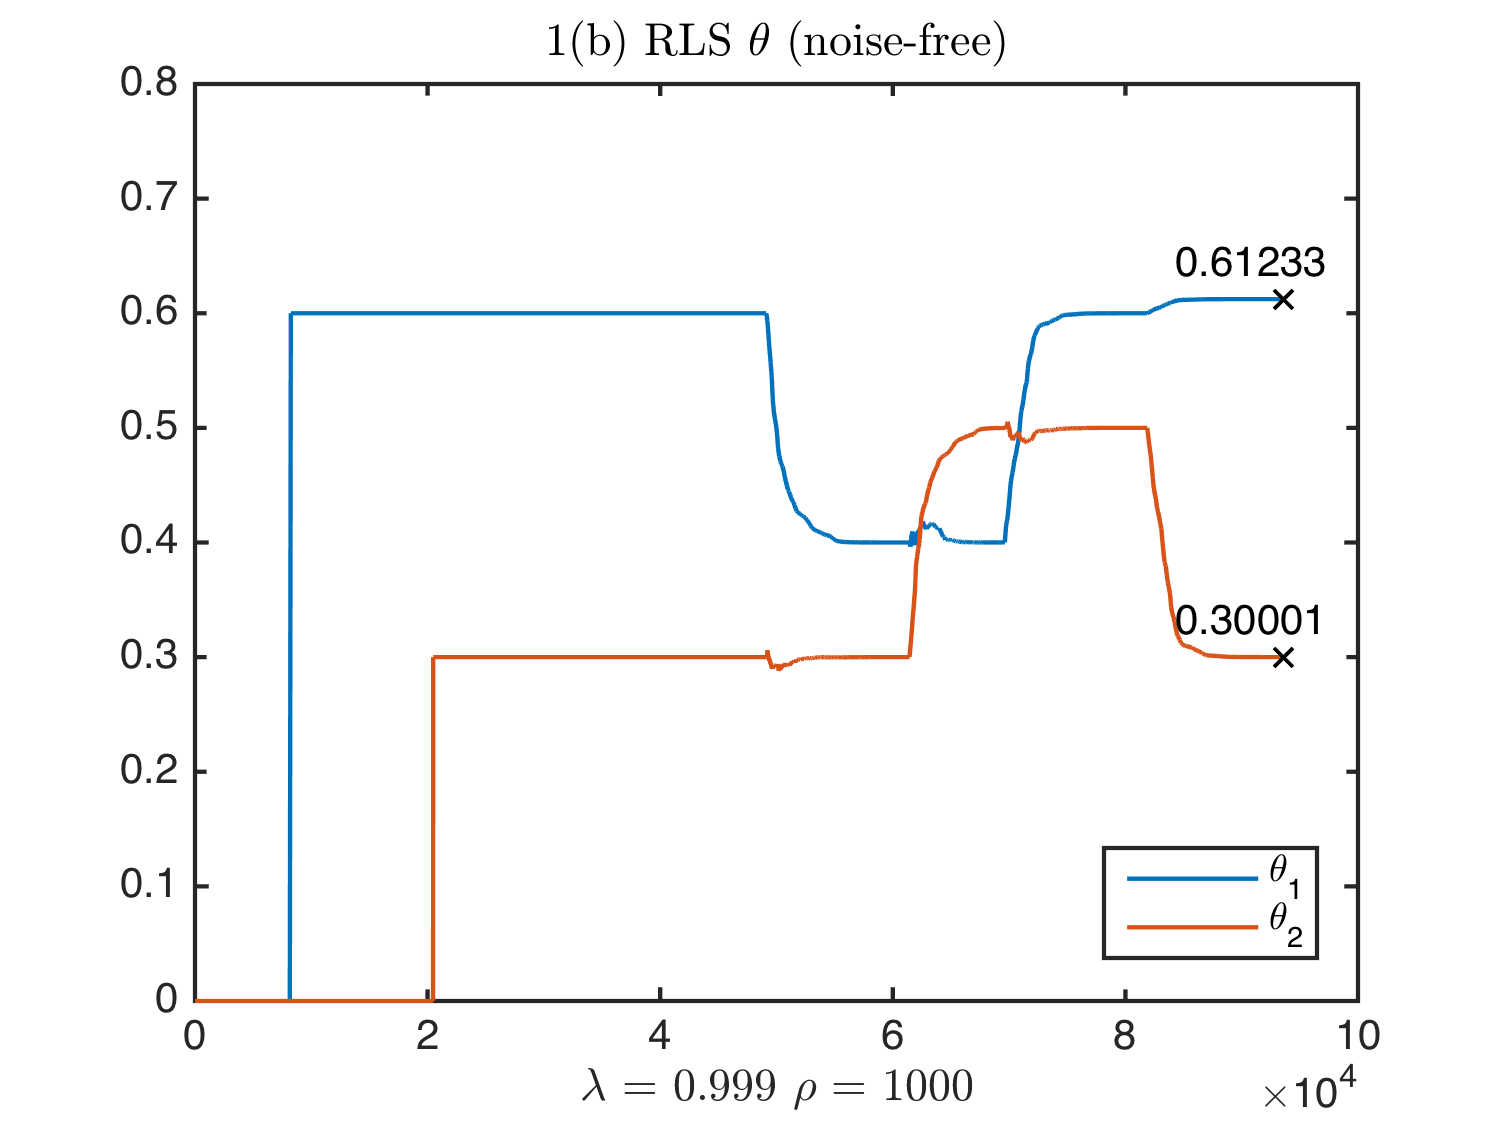
\includegraphics[width=2.5in]{b-rls-theta-noise-free}
\caption{RLS $\theta$ trends}
\label{b-rls-theta-noise-free}
\end{minipage}
\begin{minipage}[t]{0.33\linewidth}
\centering
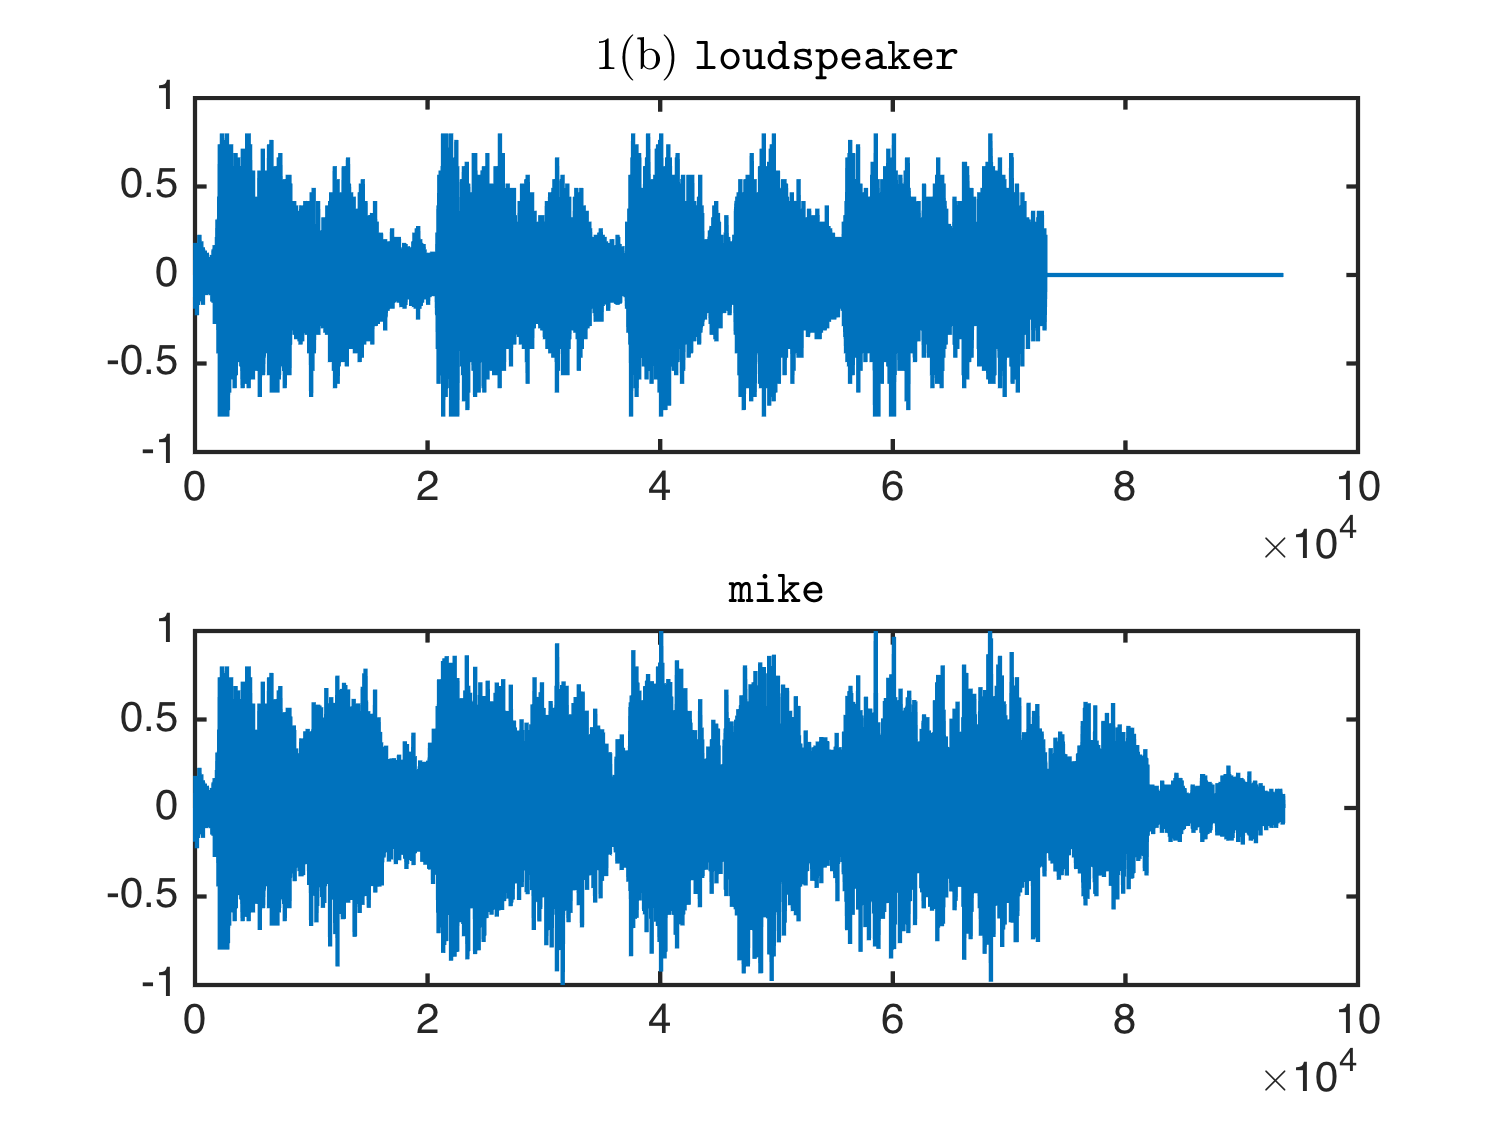
\includegraphics[width=2.5in]{b-rls-input-noise-free}
\caption{inputs}
\end{minipage}
\begin{minipage}[t]{0.33\linewidth}
\centering
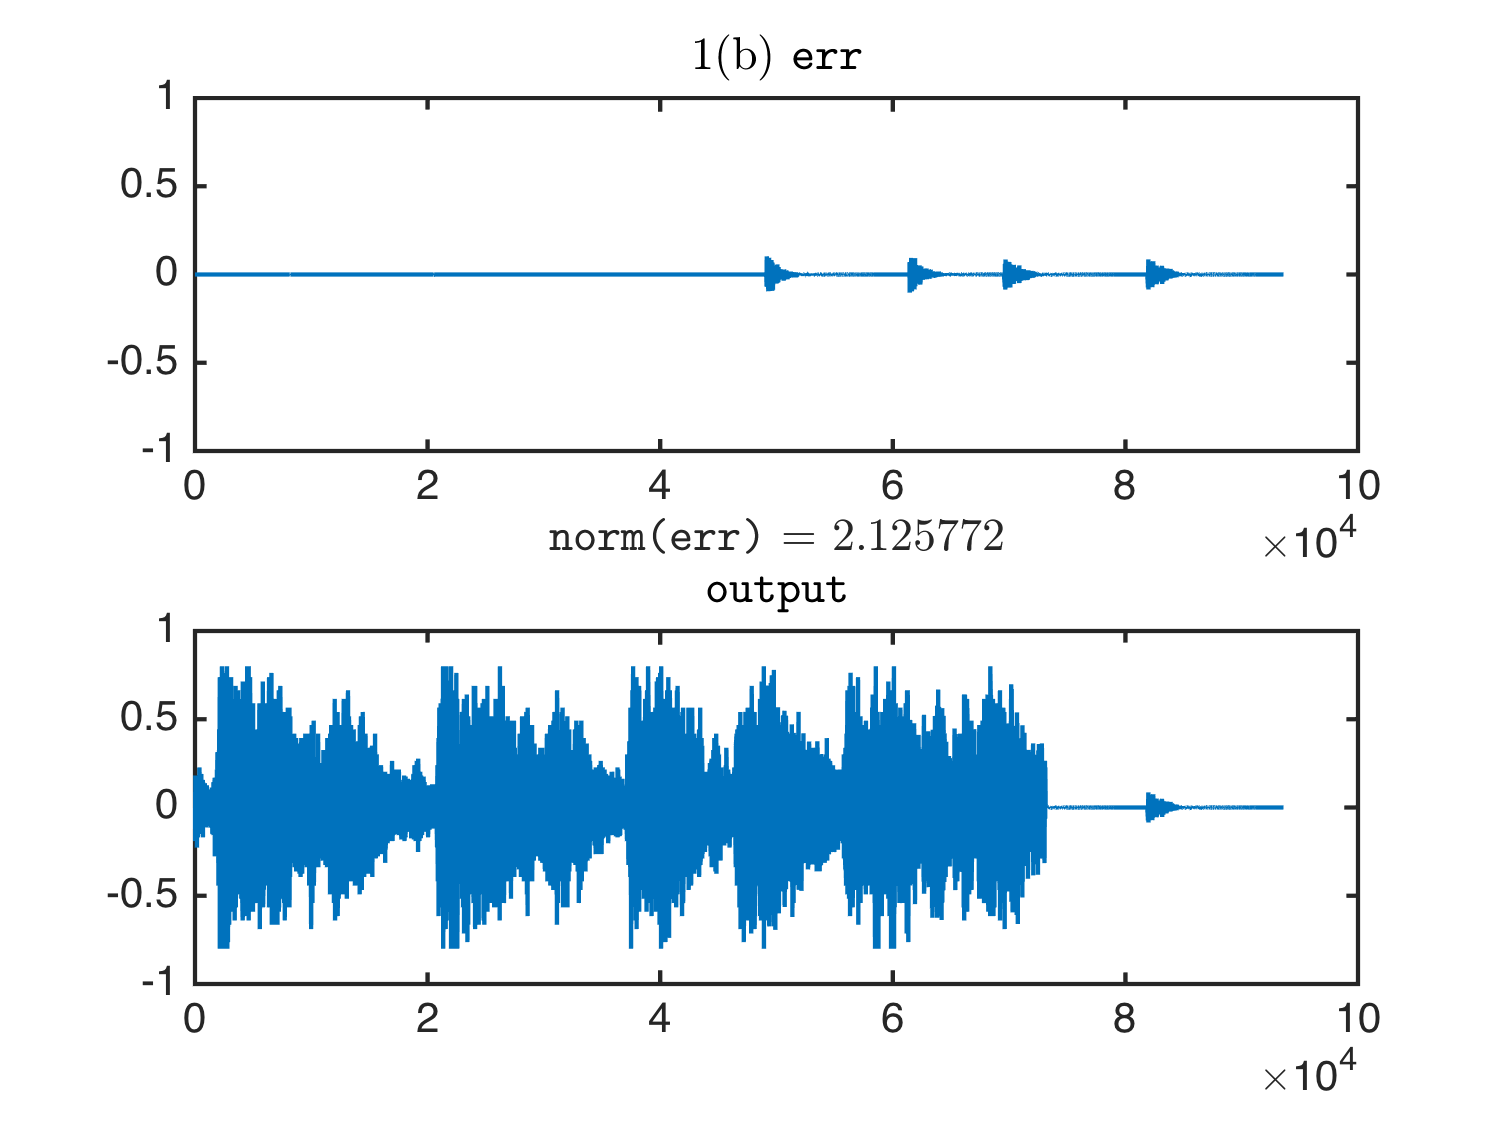
\includegraphics[width=2.5in]{b-rls-output-noise-free}
\caption{output and comparison}
\label{b-rls-output-noise-free}
\end{minipage}
\end{figure}

In Fig. \ref{b-rls-theta-noise-free}, $\theta_1$ and $\theta_2$ eventually converge to 0.612 and 0.300. In Fig. \ref{b-rls-output-noise-free}, echoes are successfully suppressed and \texttt{err} is negligible comparing with \texttt{mike2}.

%--------------------------------------------

\subsubsection*{Noisy environment}

By trial and error, we find when $\lambda = 0.999$, $\rho = 0.6$, the RLS filter has best echo-cancellation performance.
\begin{center}
\texttt{norm(err)} = 5.294251 $>$ 2.125772
\end{center}
\texttt{norm(err)} increases due to the interference of the background noise.

\begin{figure}[H]
\begin{minipage}[t]{0.33\linewidth}
\centering
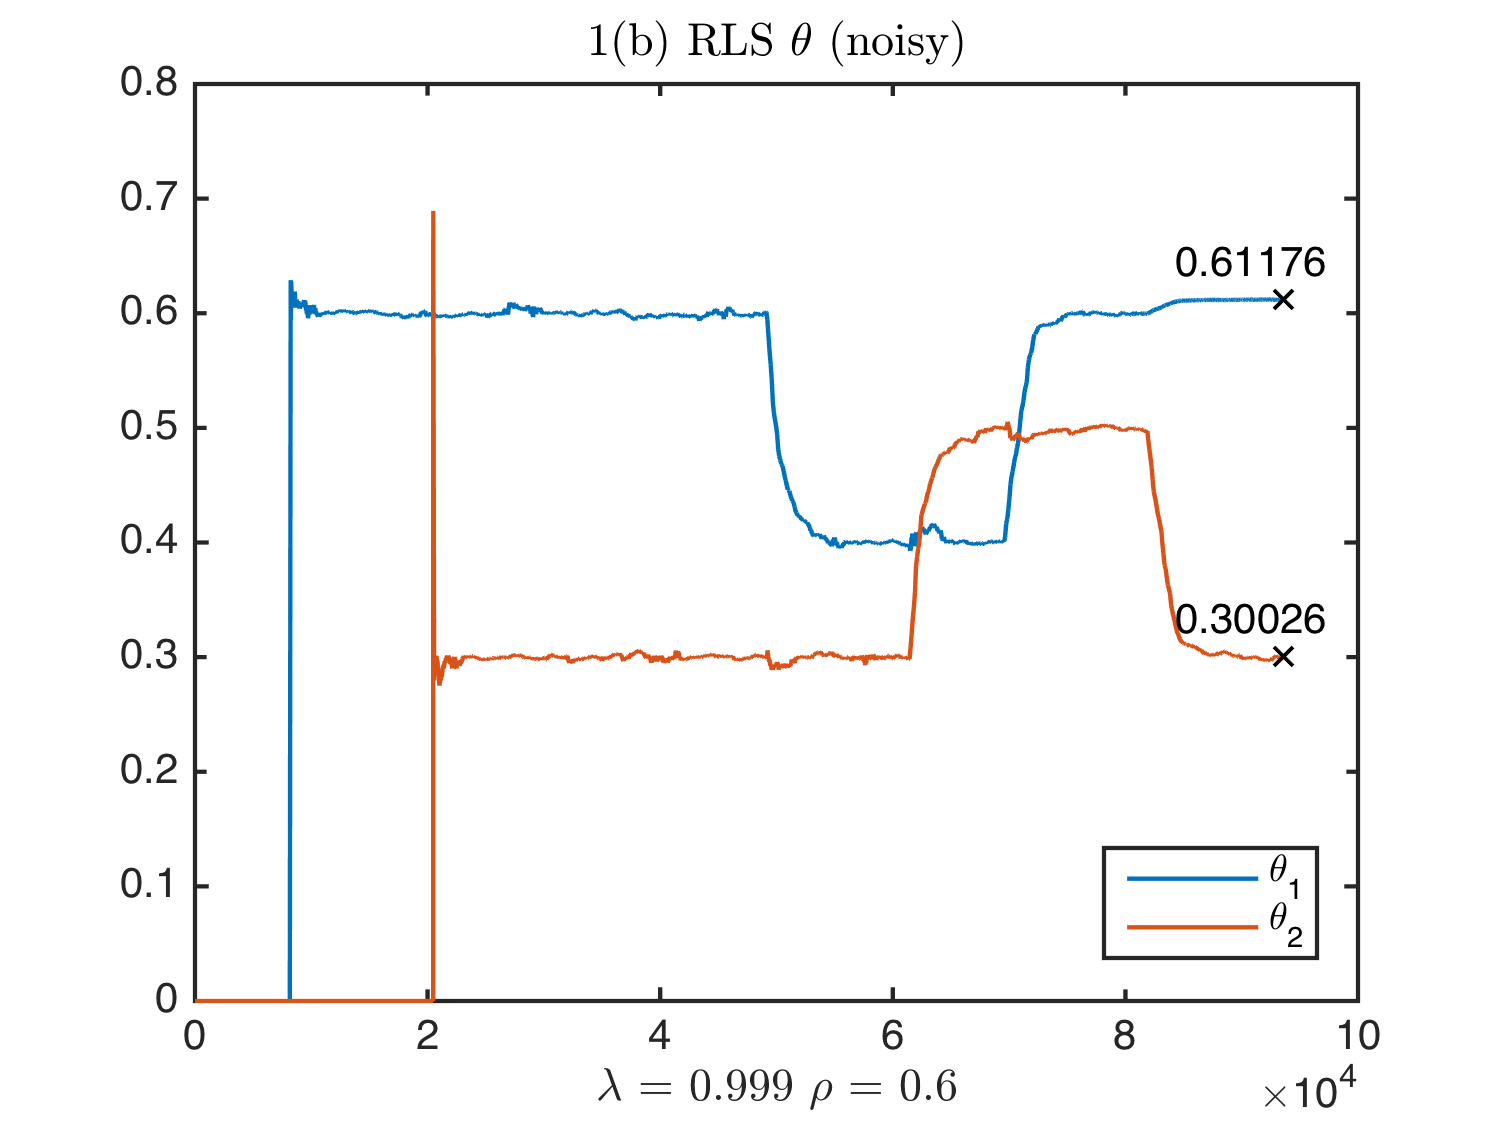
\includegraphics[width=2.5in]{b-rls-theta-noisy}
\caption{RLS $\theta$ trends}
\label{b-rls-theta-noisy}
\end{minipage}
\begin{minipage}[t]{0.33\linewidth}
\centering
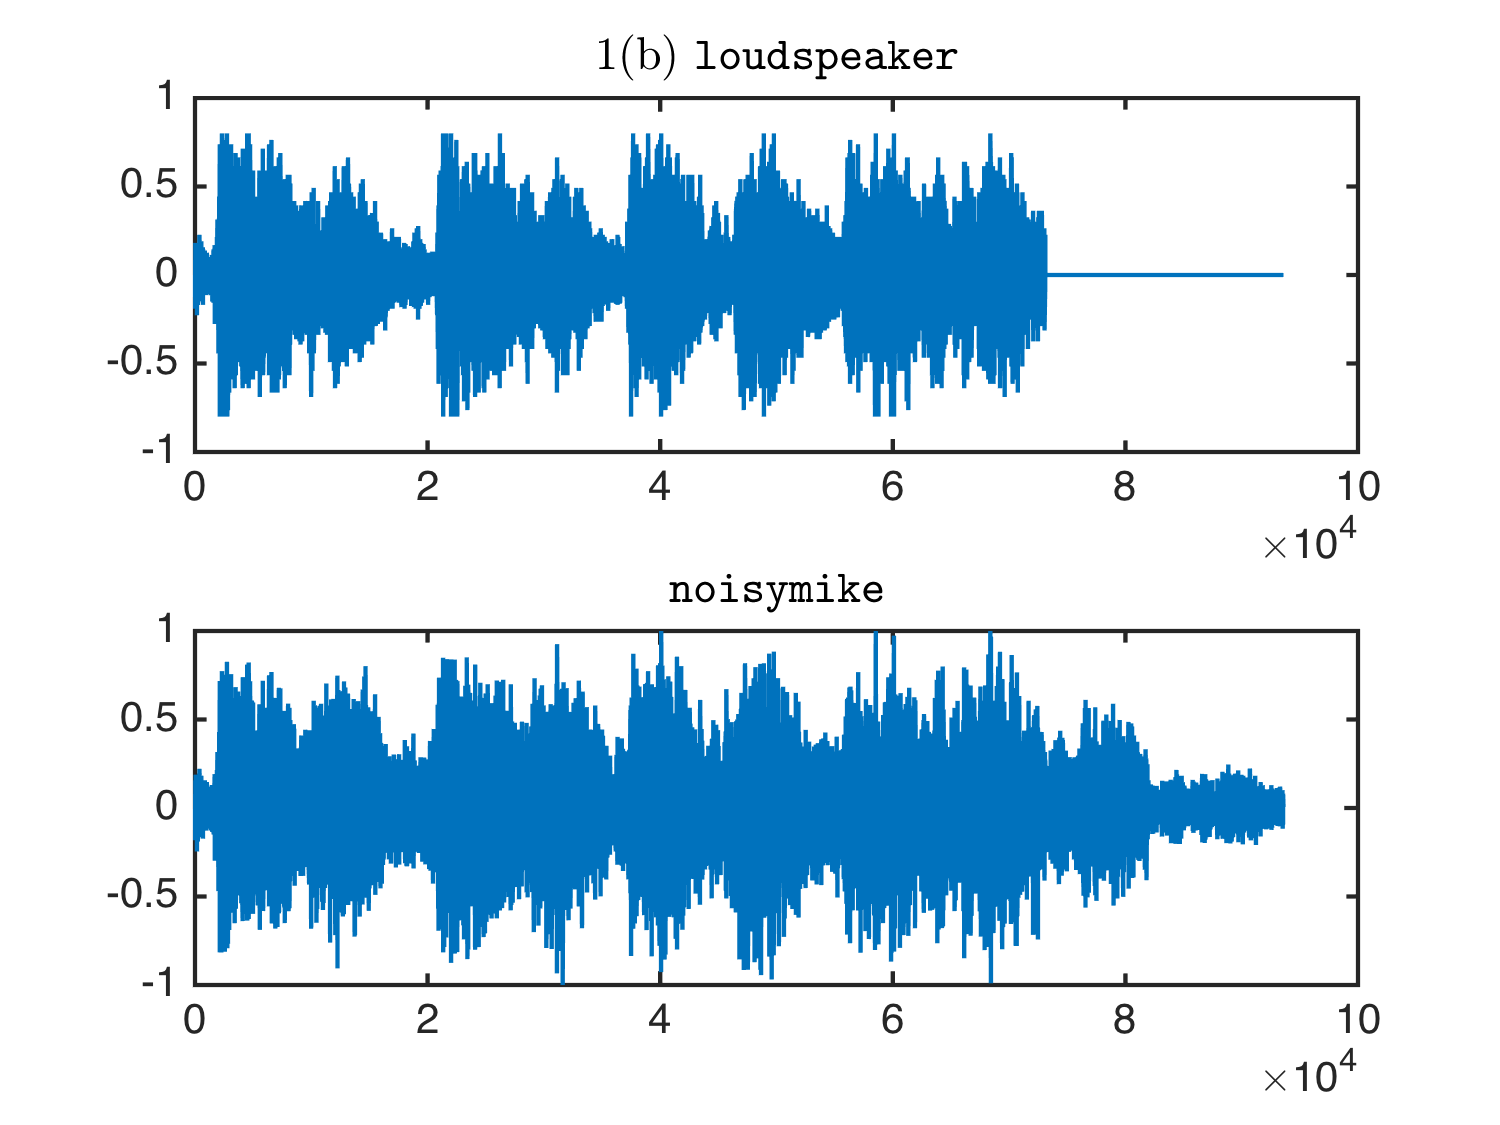
\includegraphics[width=2.5in]{b-rls-input-noisy}
\caption{inputs}
\end{minipage}
\begin{minipage}[t]{0.33\linewidth}
\centering
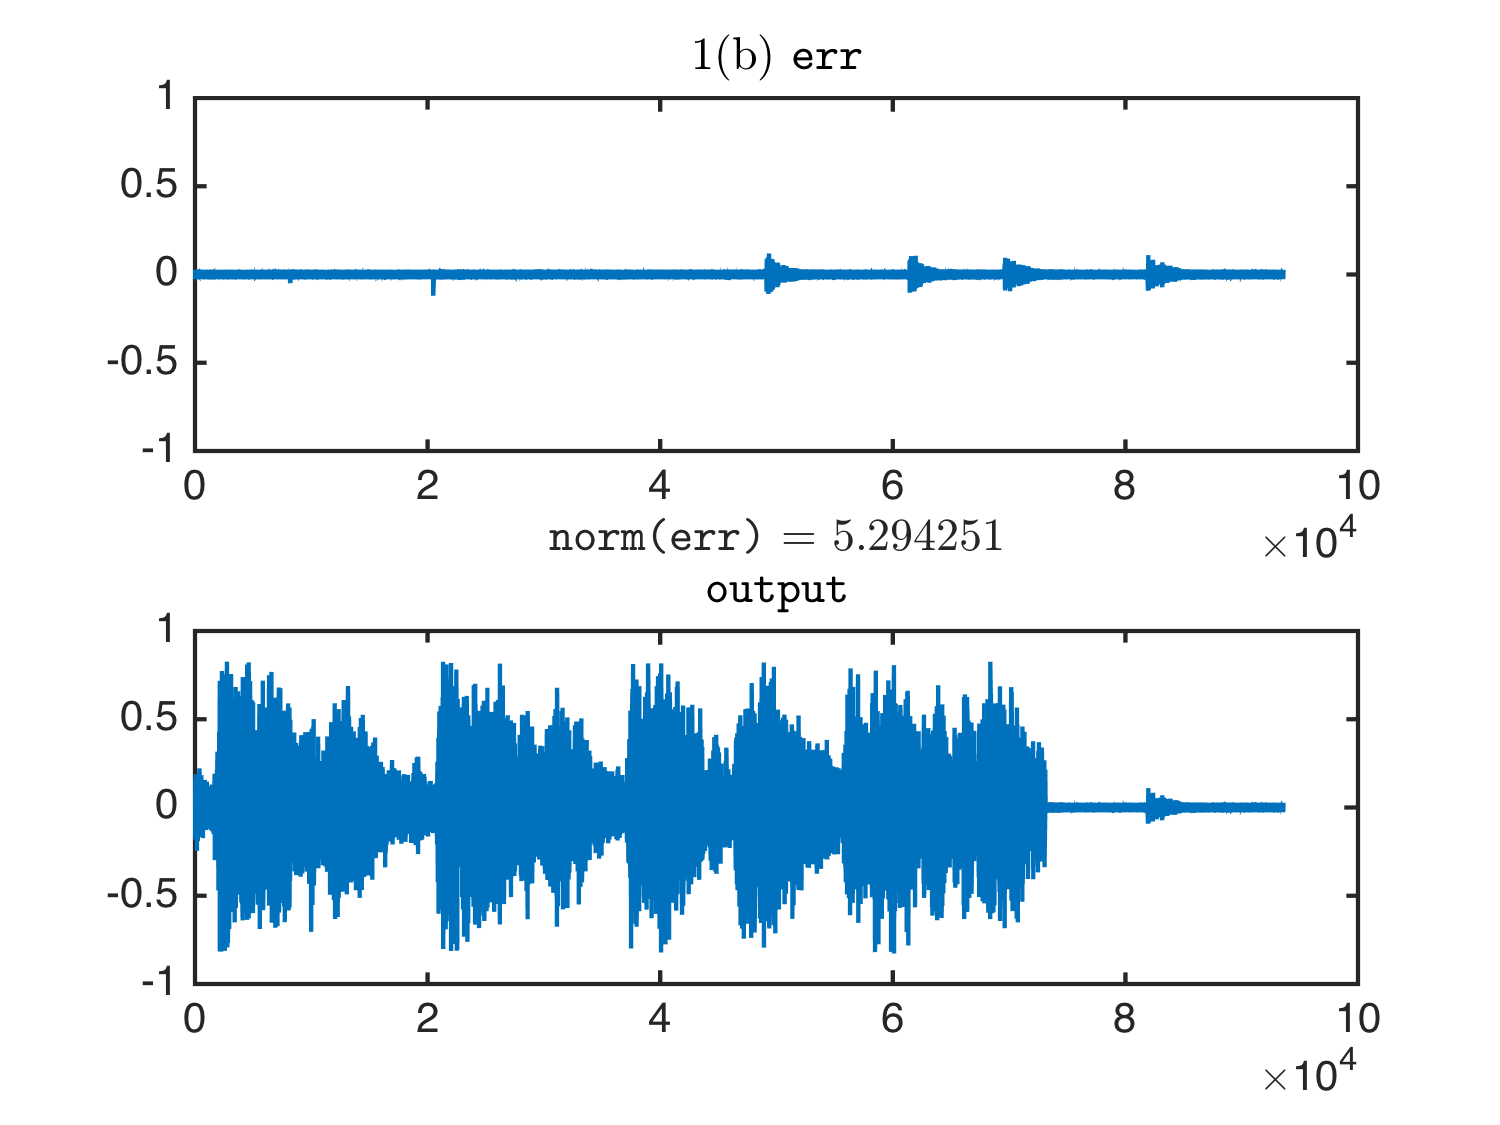
\includegraphics[width=2.5in]{b-rls-output-noisy}
\caption{output and comparison}
\label{b-rls-output-noisy}
\end{minipage}
\end{figure}

In Fig. \ref{b-rls-theta-noisy}, $\theta_1$ and $\theta_2$ eventually converge to 0.612 and 0.300. In Fig. \ref{b-rls-output-noisy}, echoes are successfully suppressed and \texttt{err} is negligible comparing with \texttt{noisymike2}.

%--------------------------------------------
%--------------------------------------------

\subsection*{LMS}

\subsubsection*{Noise-free environment}

By trial and error, we find when \texttt{step\_size} = 2$\mu$ = 10, the LMS filter has best echo-cancellation performance.
\begin{center}
\texttt{norm(err)} = 0.210652
\end{center}

\begin{figure}[H]
\begin{minipage}[t]{0.33\linewidth}
\centering
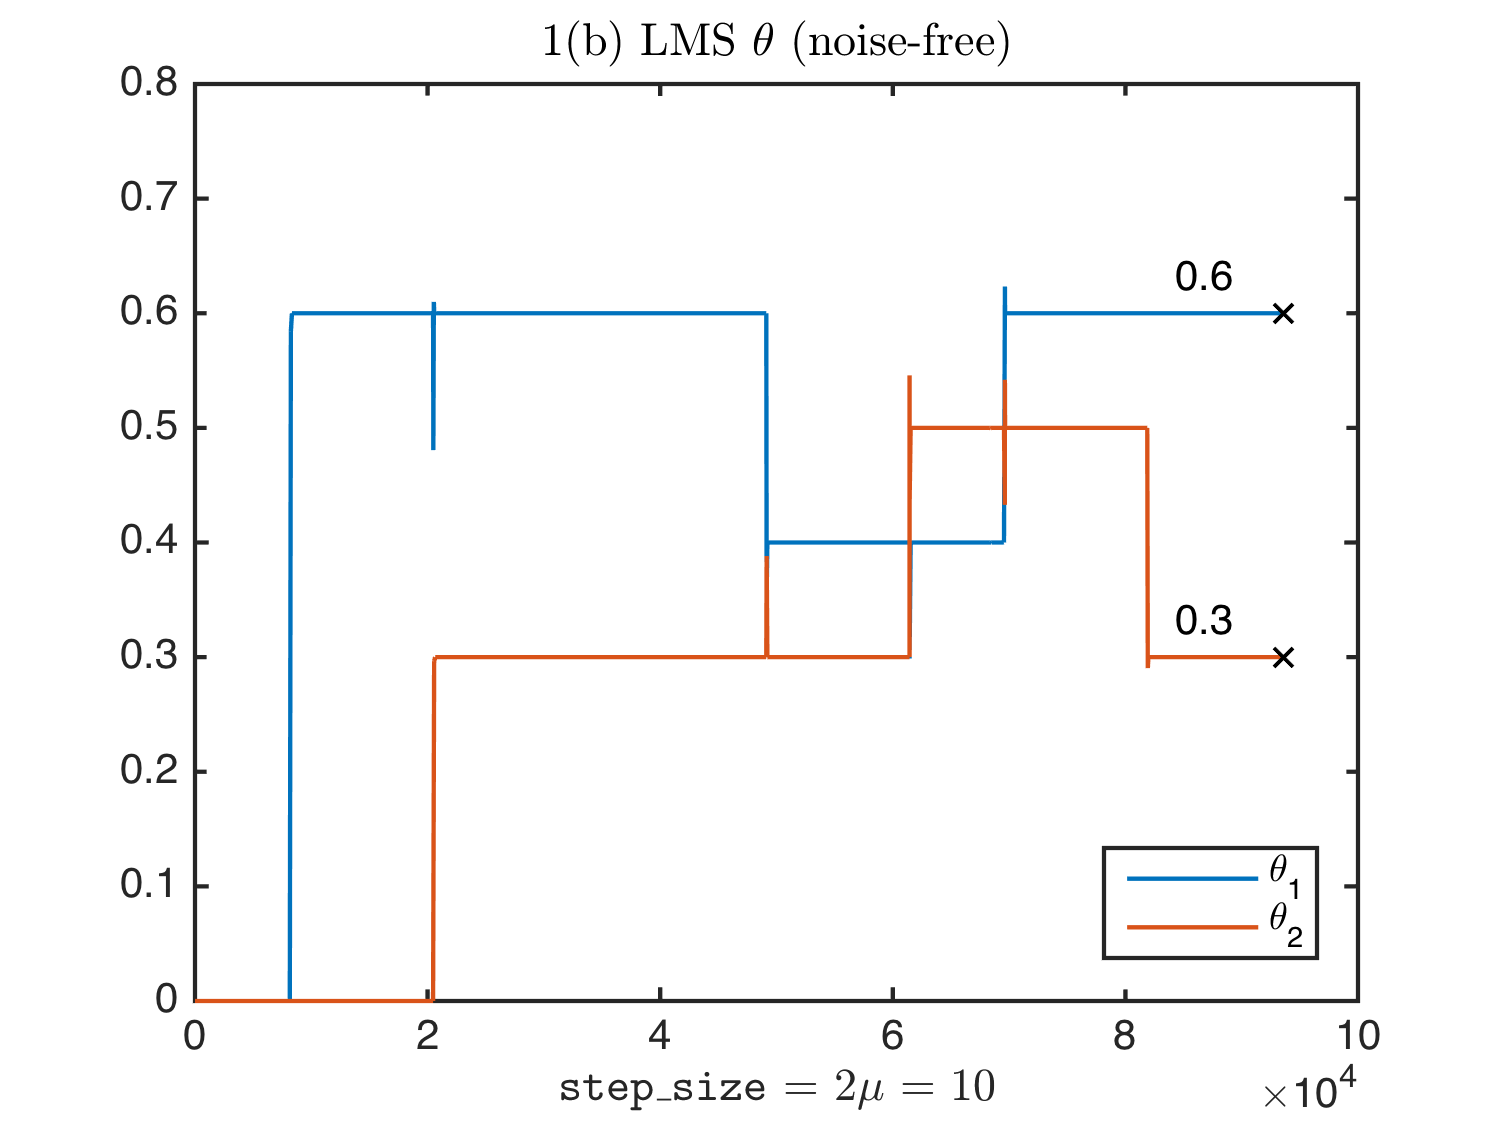
\includegraphics[width=2.5in]{b-lms-theta-noise-free}
\caption{LMS $\theta$ trends}
\label{b-lms-theta-noise-free}
\end{minipage}
\begin{minipage}[t]{0.33\linewidth}
\centering
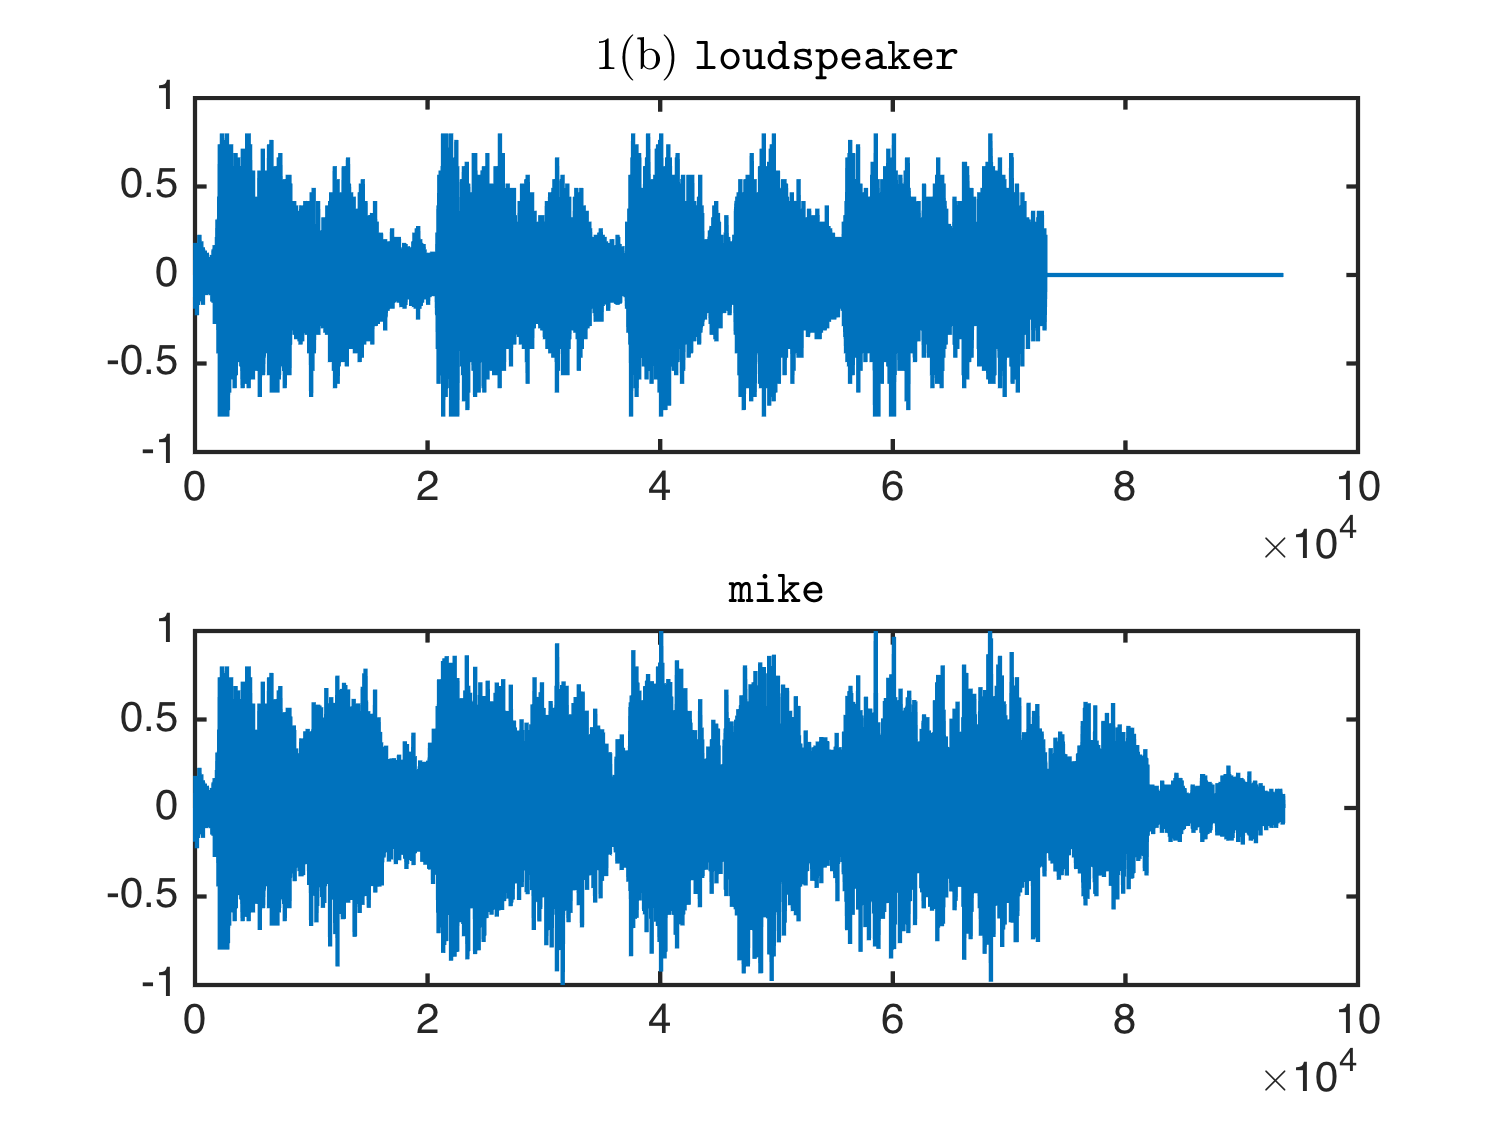
\includegraphics[width=2.5in]{b-lms-input-noise-free}
\caption{inputs}
\end{minipage}
\begin{minipage}[t]{0.33\linewidth}
\centering
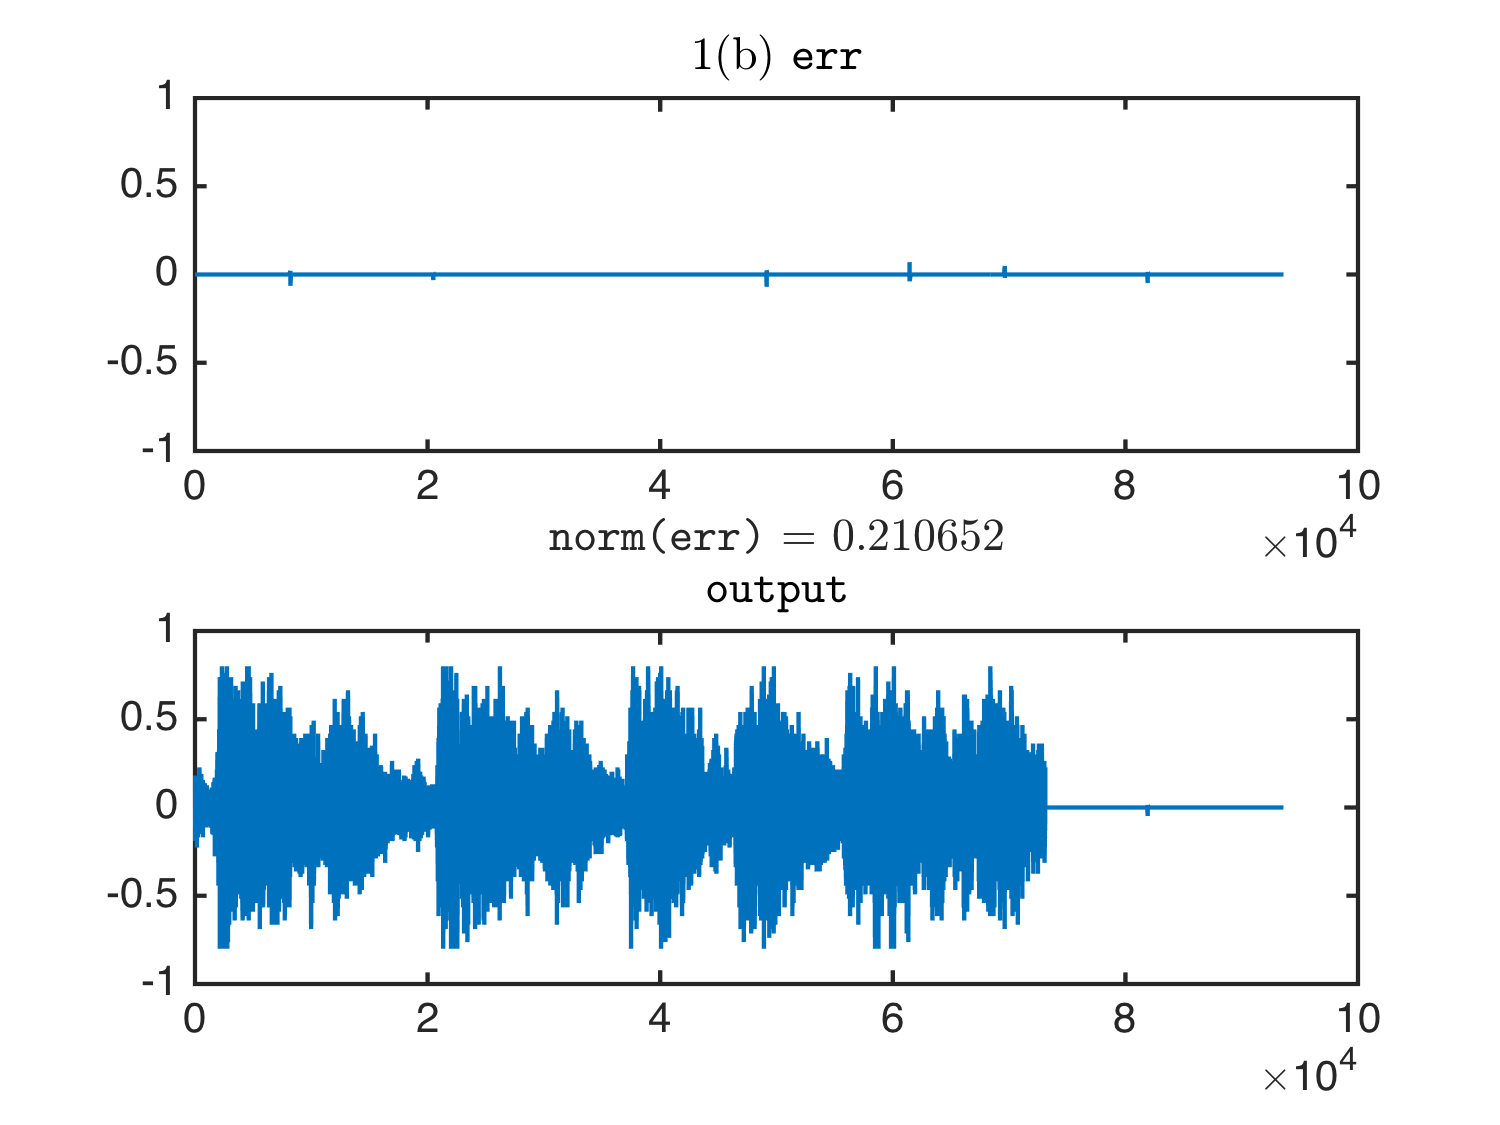
\includegraphics[width=2.5in]{b-lms-output-noise-free}
\caption{output and comparison}
\label{b-lms-output-noise-free}
\end{minipage}
\end{figure}

In Fig. \ref{b-lms-theta-noise-free}, $\theta_1$ and $\theta_2$ eventually converge to 0.6 and 0.3. In Fig. \ref{b-lms-output-noise-free}, echoes are successfully suppressed and \texttt{err} is negligible comparing with \texttt{mike2}.

%--------------------------------------------

\subsubsection*{Noisy environment}

By trial and error, we find when \texttt{step\_size} = 2$\mu$ = 0.6, the LMS filter has best echo-cancellation performance.
\begin{center}
\texttt{norm(err)} = 4.943508 $>$ 0.210652
\end{center}
\texttt{norm(err)} increases due to the interference of the background noise.

\begin{figure}[H]
\begin{minipage}[t]{0.33\linewidth}
\centering
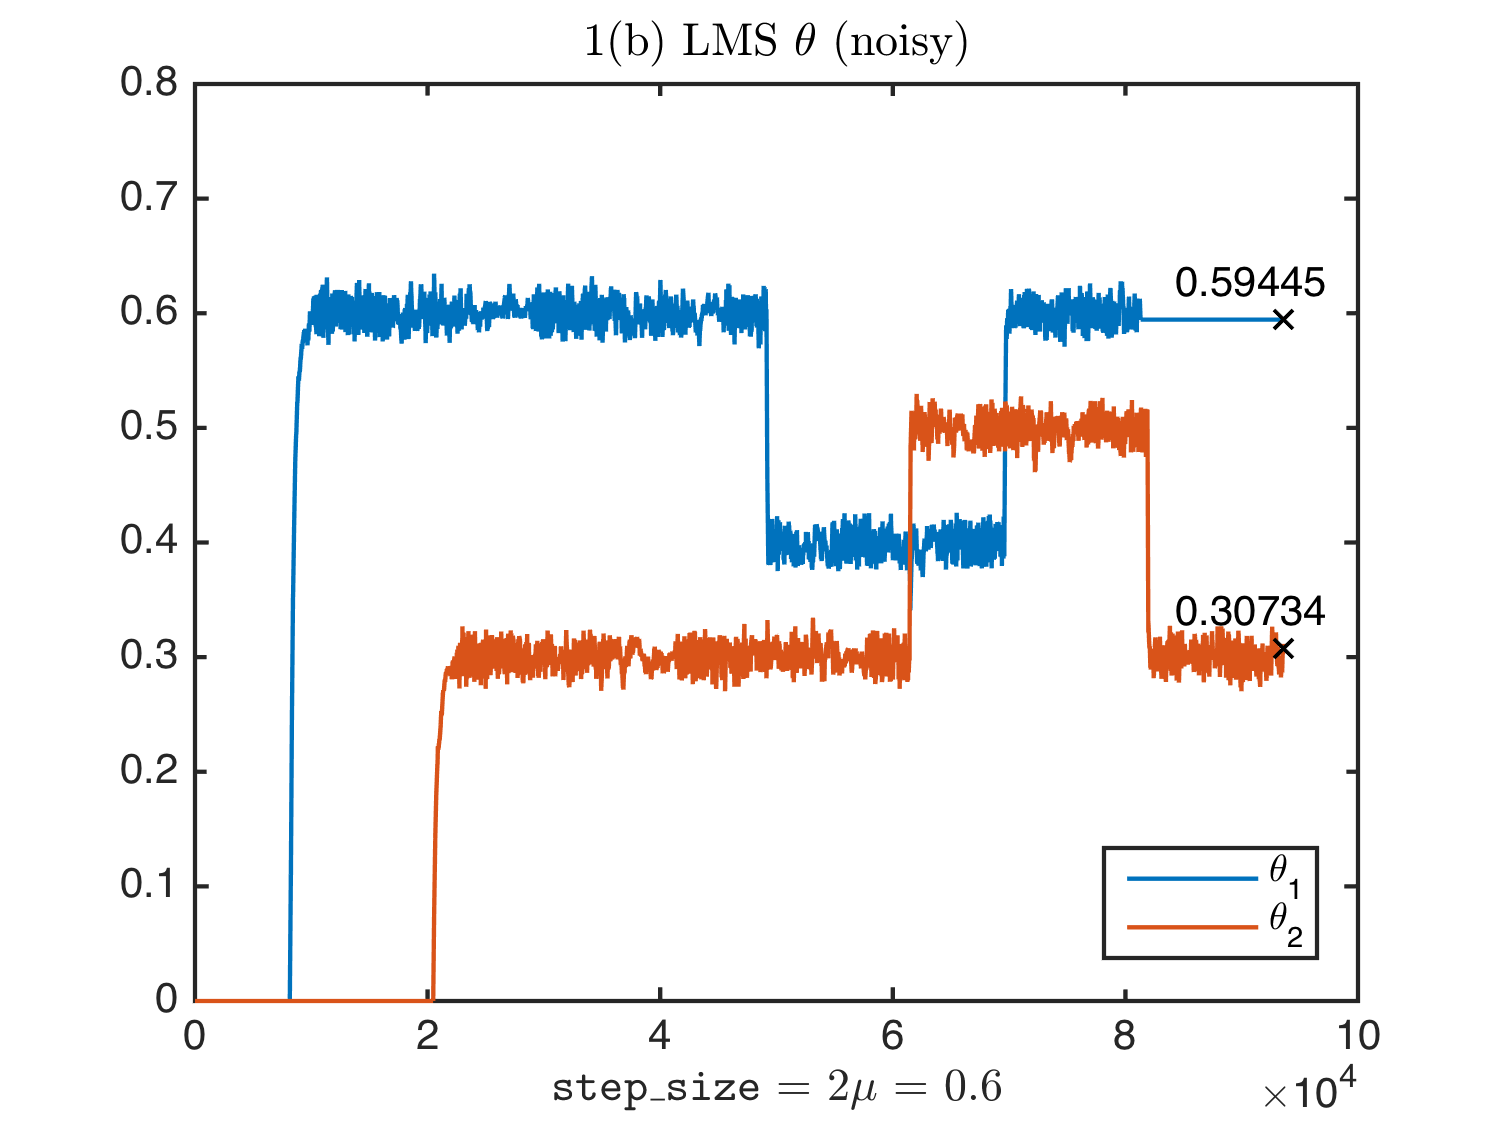
\includegraphics[width=2.5in]{b-lms-theta-noisy}
\caption{LMS $\theta$ trends}
\label{b-lms-theta-noisy}
\end{minipage}
\begin{minipage}[t]{0.33\linewidth}
\centering
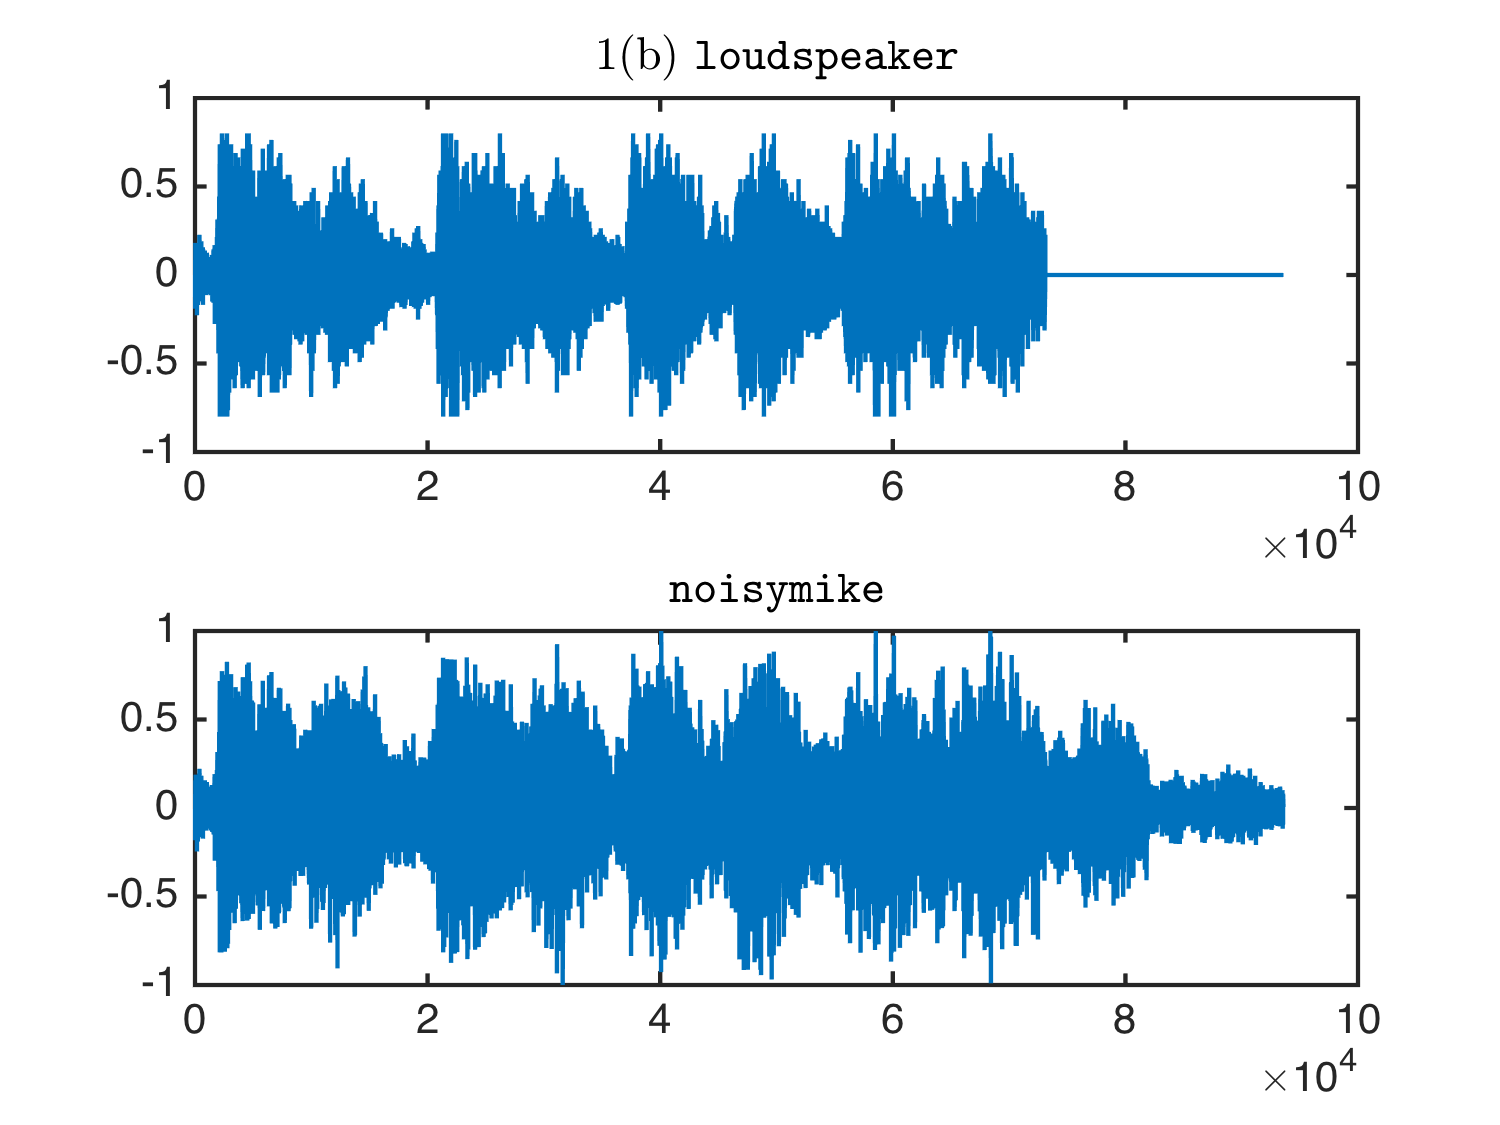
\includegraphics[width=2.5in]{b-lms-input-noisy}
\caption{inputs}
\end{minipage}
\begin{minipage}[t]{0.33\linewidth}
\centering
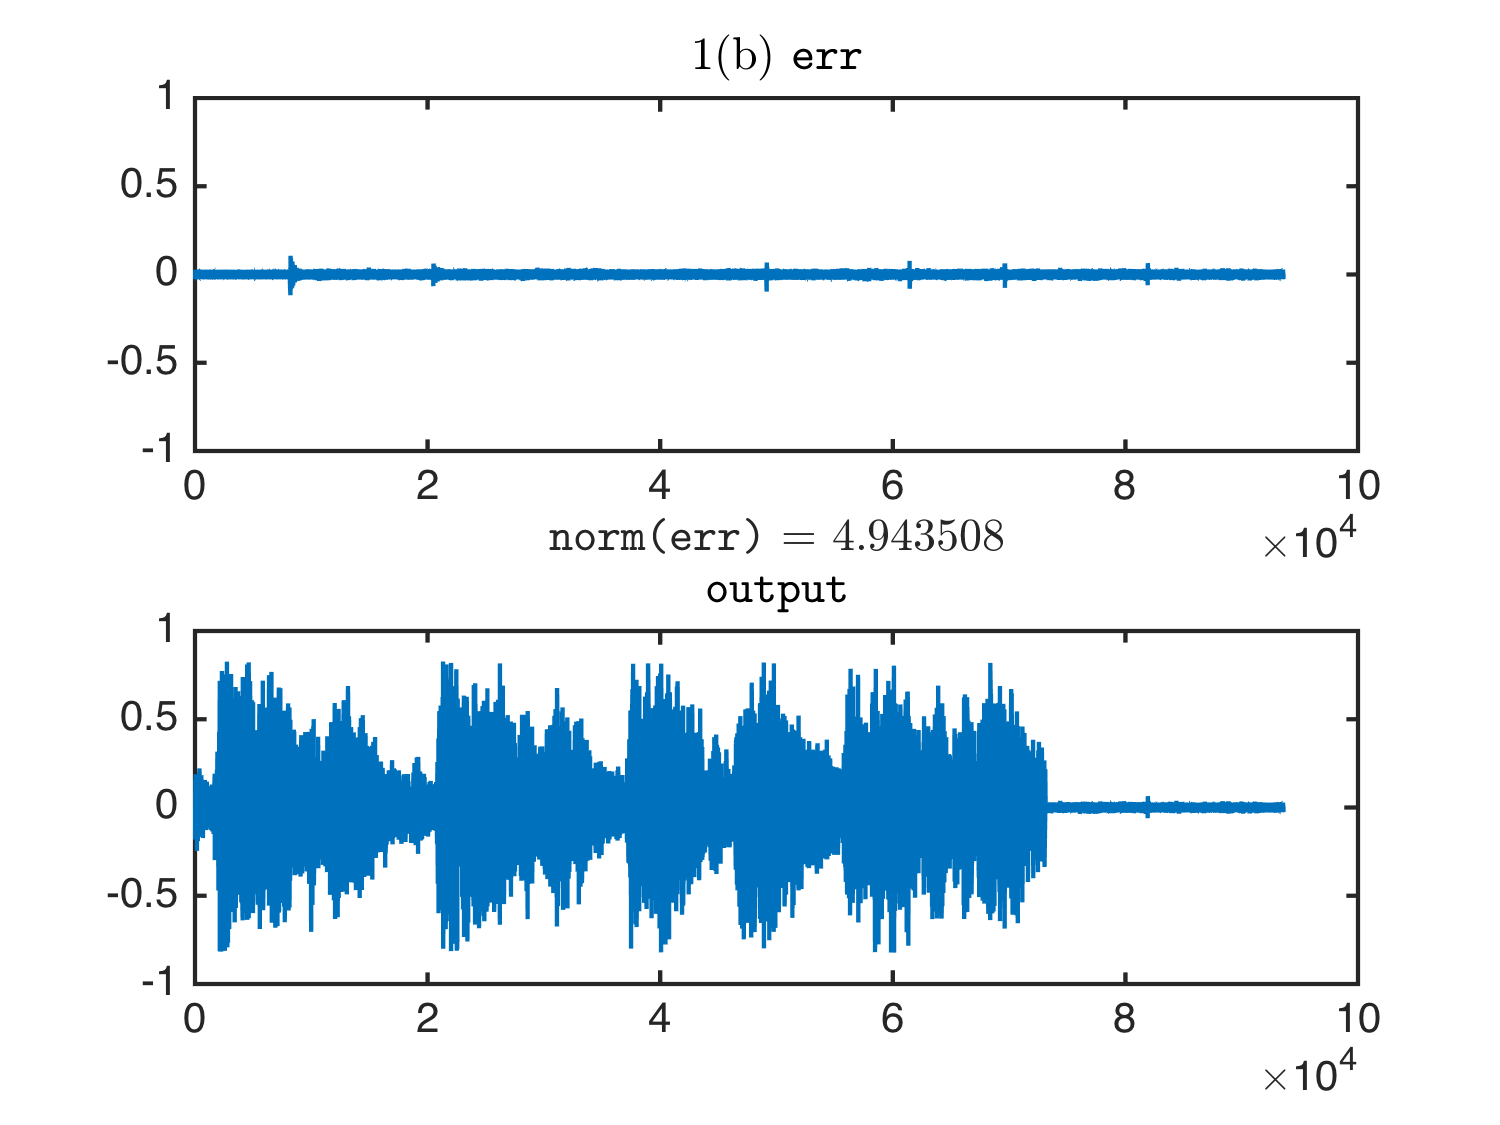
\includegraphics[width=2.5in]{b-lms-output-noisy}
\caption{output and comparison}
\label{b-lms-output-noisy}
\end{minipage}
\end{figure}

In Fig. \ref{b-lms-theta-noisy}, $\theta_1$ and $\theta_2$ eventually converge to 0.594 and 0.307. In Fig. \ref{b-lms-output-noisy}, echoes are successfully suppressed and \texttt{err} is negligible comparing with \texttt{noisymike2}.

%--------------------------------------------
%--------------------------------------------

\subsection*{RLS \& LMS comparison}
As is shown in Fig. \ref{b-rls-theta-noise-free} and Fig. \ref{b-lms-theta-noise-free}, $\theta$ in LMS converges faster than RLS because LMS focus more on recent data points. As a result, when the echo amplitude is time-varying, LMS can react more nimbly than RLS. In fact, \texttt{norm(err)} of LMS is smaller than RLS (0.210652 vs 2.125772).

%----------------------------------------------------------------------------------------
%	Task 1 (c)
%----------------------------------------------------------------------------------------

\section*{Task 1 (c) unknown delay}

\subsection*{RLS}

\begin{equation*}
0.001 \times 8192 \approx 8
\end{equation*}

New filter length
\begin{equation*}
2 \times (8 + 1 + 8) = 34
\end{equation*}

We will only plot trends of $\theta_9$ ($9 = 8 + 1$) and $\theta_{26}$ ($26 = (8 + 1 + 8) + 8 + 1$), because other values of $\theta$ are approximate 0.

\subsubsection*{Noise-free environment}

By trial and error, we find when $\lambda = 0.999$, $\rho = 100$, the RLS filter has best echo-cancellation performance.
\begin{center}
\texttt{norm(err)} = 2.074119
\end{center}

\begin{figure}[H]
\begin{minipage}[t]{0.33\linewidth}
\centering
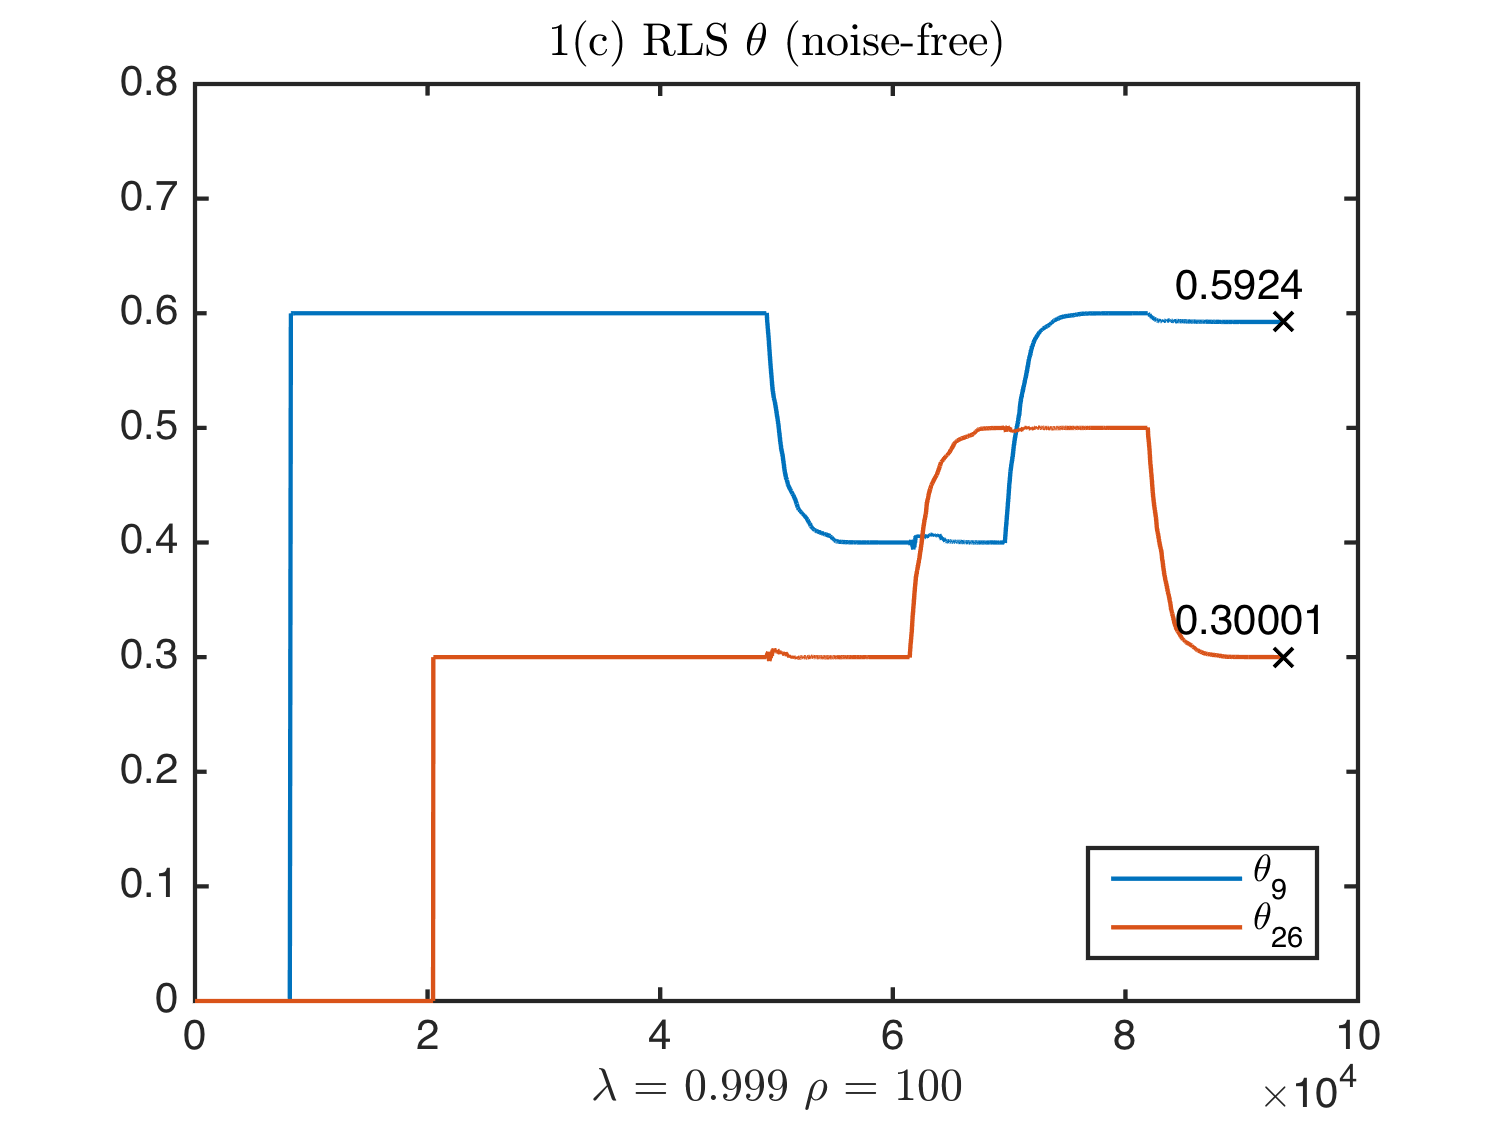
\includegraphics[width=2.5in]{c-rls-theta-noise-free}
\caption{RLS $\theta$ trends}
\label{c-rls-theta-noise-free}
\end{minipage}
\begin{minipage}[t]{0.33\linewidth}
\centering
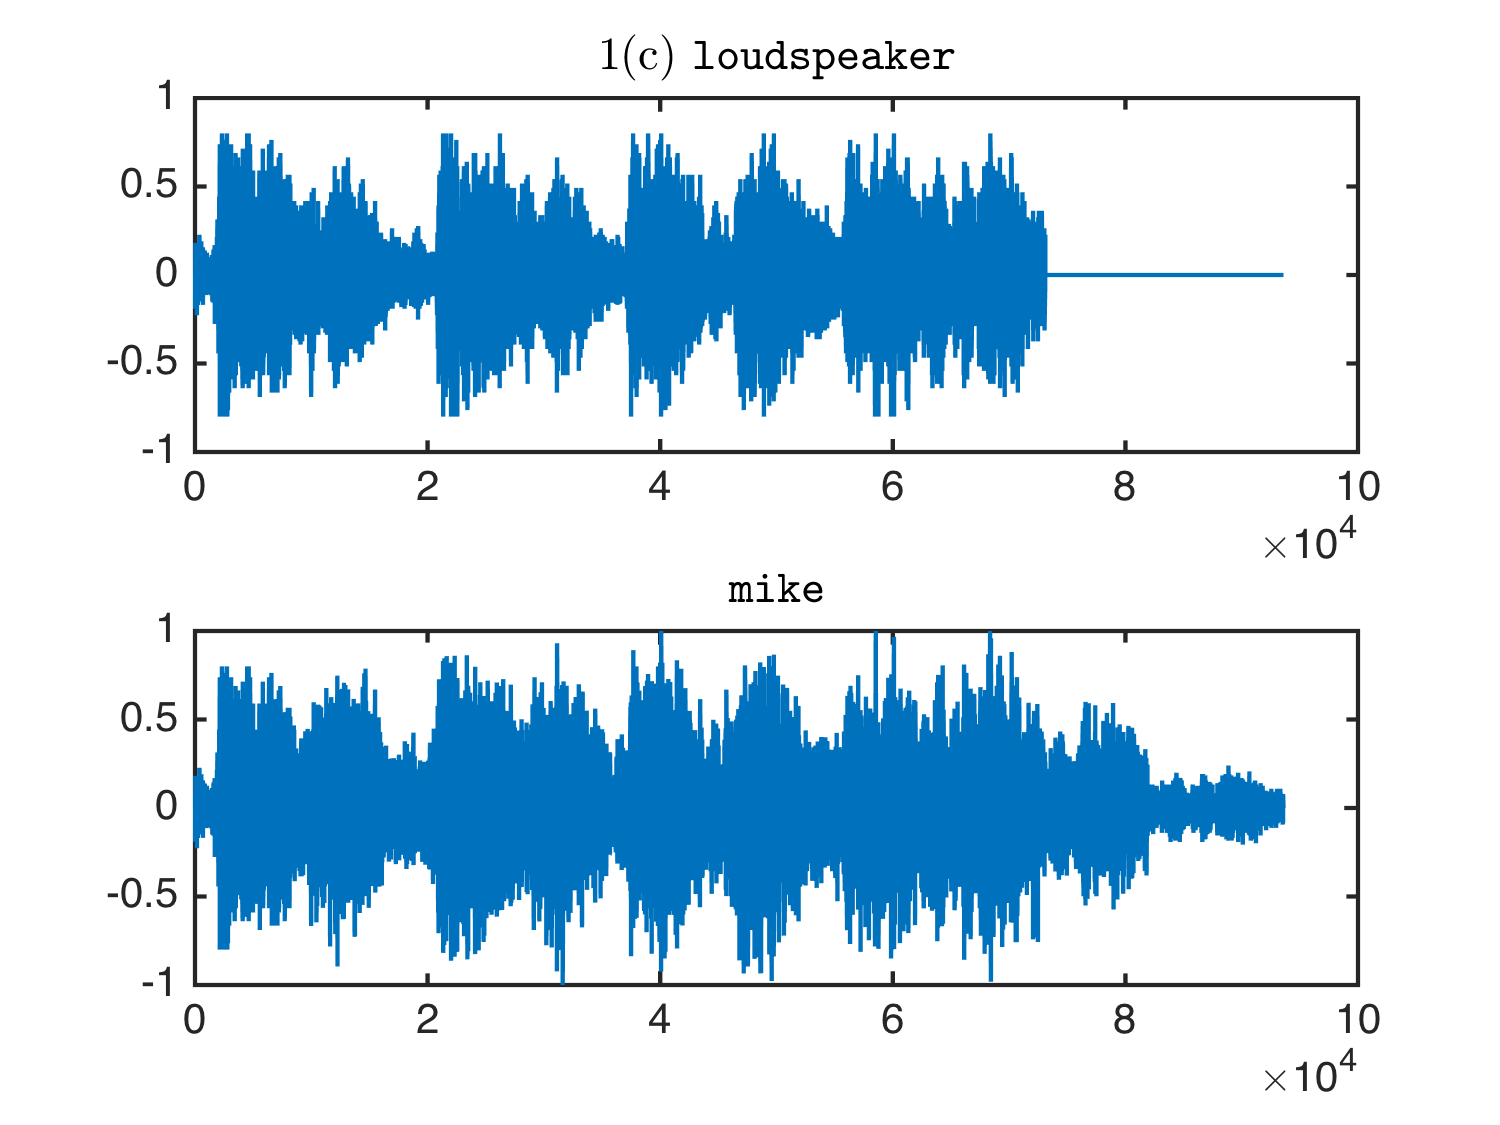
\includegraphics[width=2.5in]{c-rls-input-noise-free}
\caption{inputs}
\end{minipage}
\begin{minipage}[t]{0.33\linewidth}
\centering
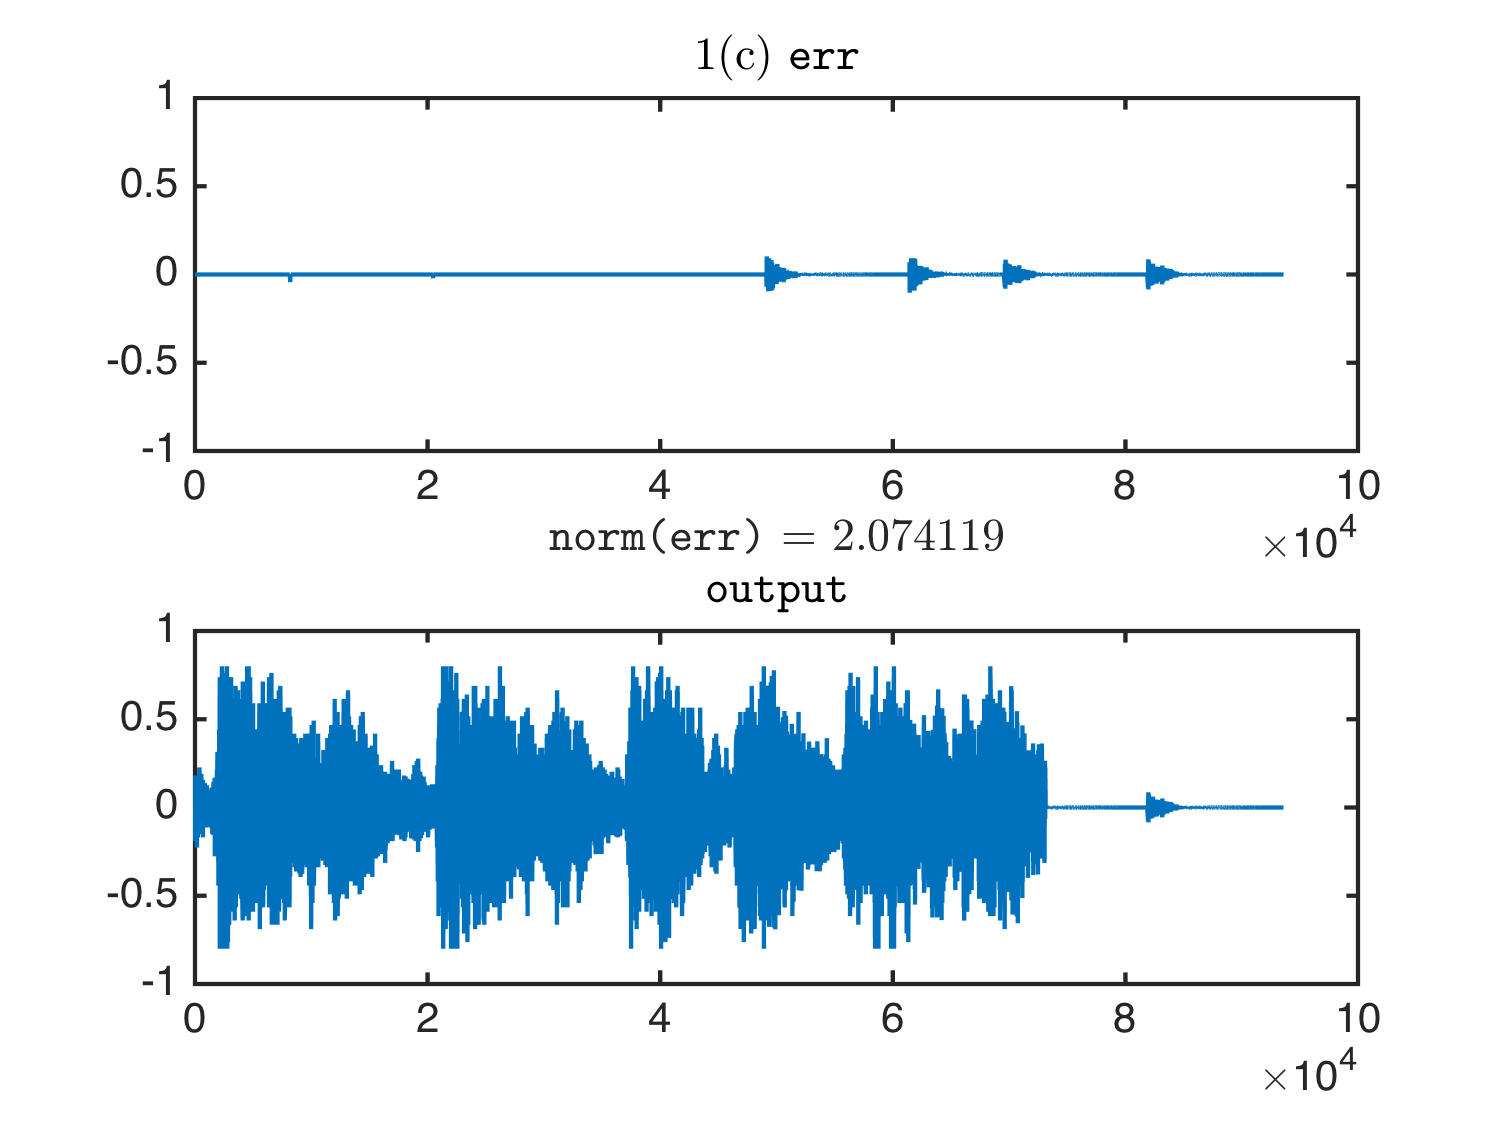
\includegraphics[width=2.5in]{c-rls-output-noise-free}
\caption{output and comparison}
\label{c-rls-output-noise-free}
\end{minipage}
\end{figure}

In Fig. \ref{c-rls-theta-noise-free}, $\theta_9$ and $\theta_{26}$ eventually converge to 0.592 and 0.300. In Fig. \ref{c-rls-output-noise-free}, echoes are successfully suppressed and \texttt{err} is negligible comparing with \texttt{mike2}.

%--------------------------------------------

\subsubsection*{Noisy environment}

By trial and error, we find when $\lambda = 0.999$, $\rho = 0.001$, the RLS filter has best echo-cancellation performance.
\begin{center}
\texttt{norm(err)} = 5.333936 $>$ 2.074119
\end{center}
\texttt{norm(err)} increases due to the interference of the background noise.

\begin{figure}[H]
\begin{minipage}[t]{0.33\linewidth}
\centering
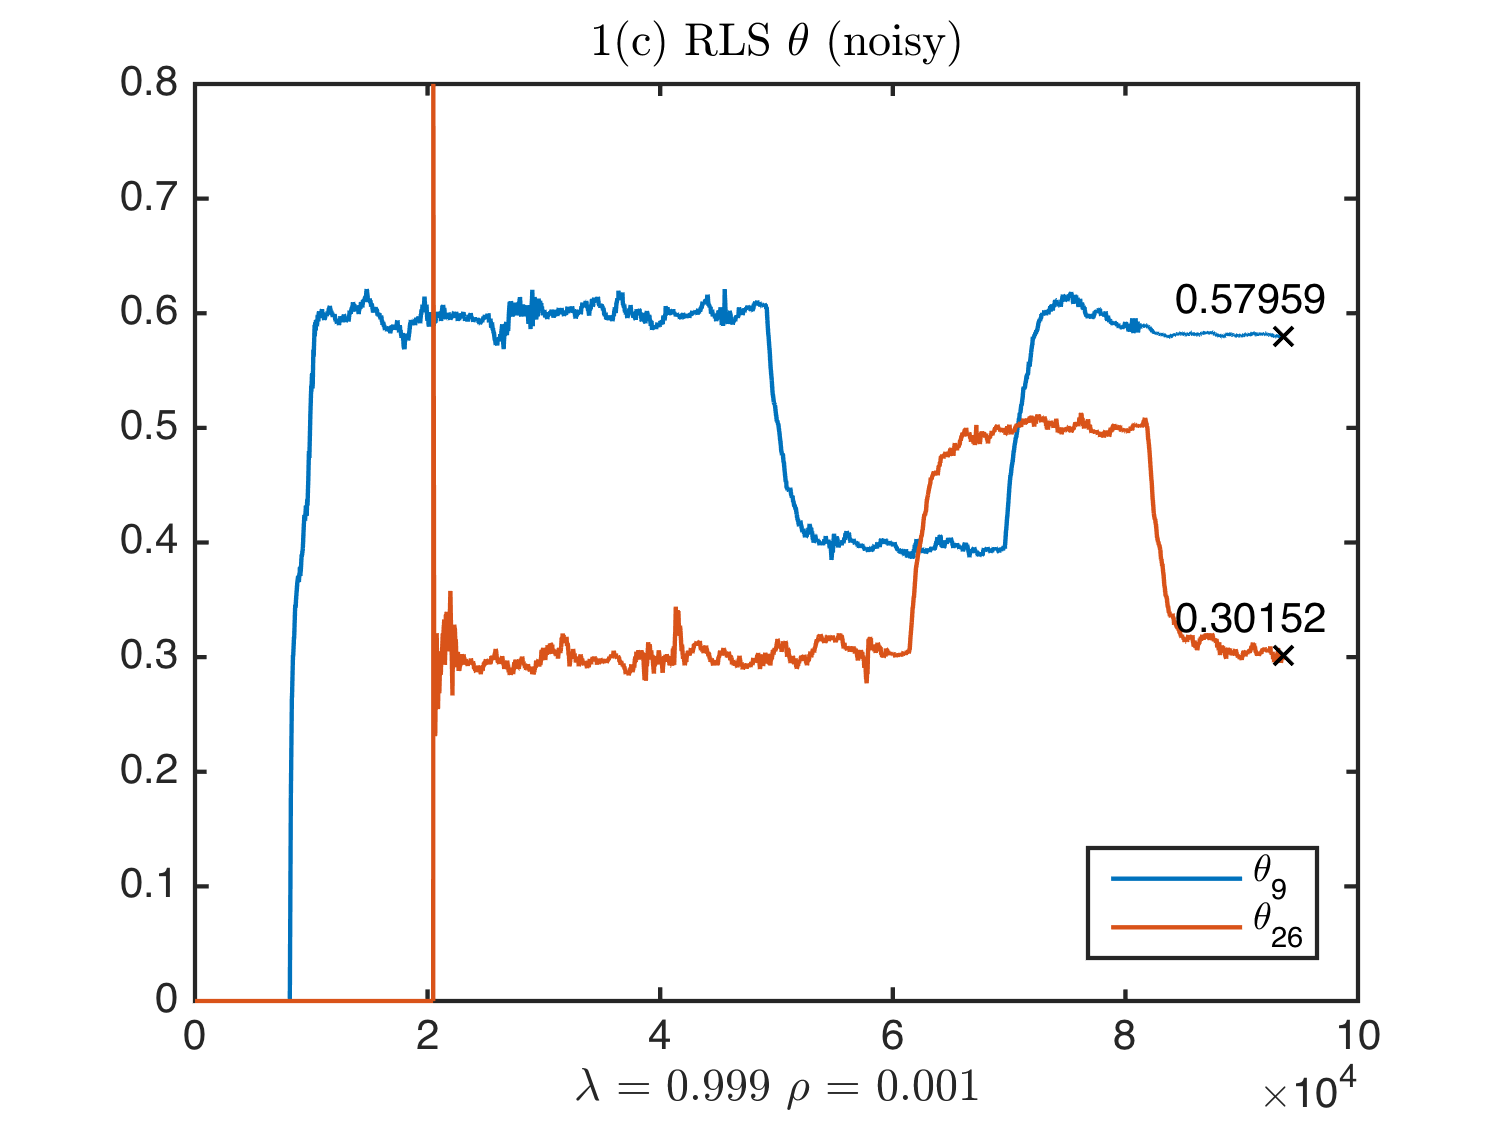
\includegraphics[width=2.5in]{c-rls-theta-noisy}
\caption{RLS $\theta$ trends}
\label{c-rls-theta-noisy}
\end{minipage}
\begin{minipage}[t]{0.33\linewidth}
\centering
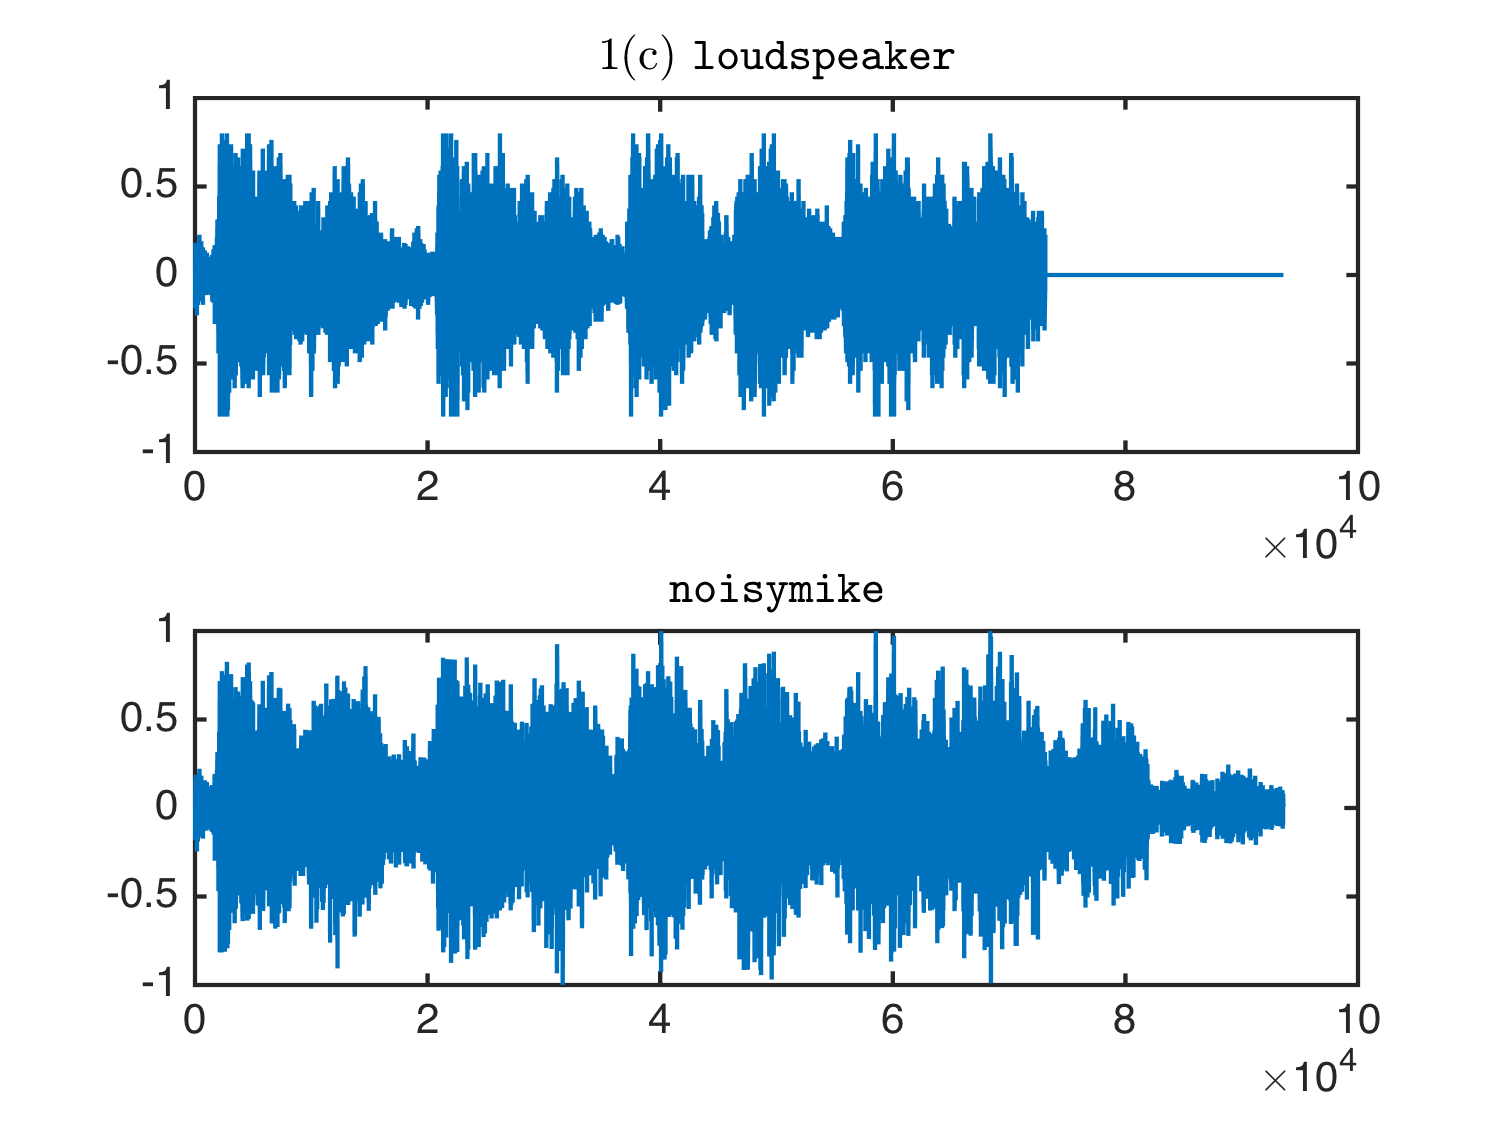
\includegraphics[width=2.5in]{c-rls-input-noisy}
\caption{inputs}
\end{minipage}
\begin{minipage}[t]{0.33\linewidth}
\centering
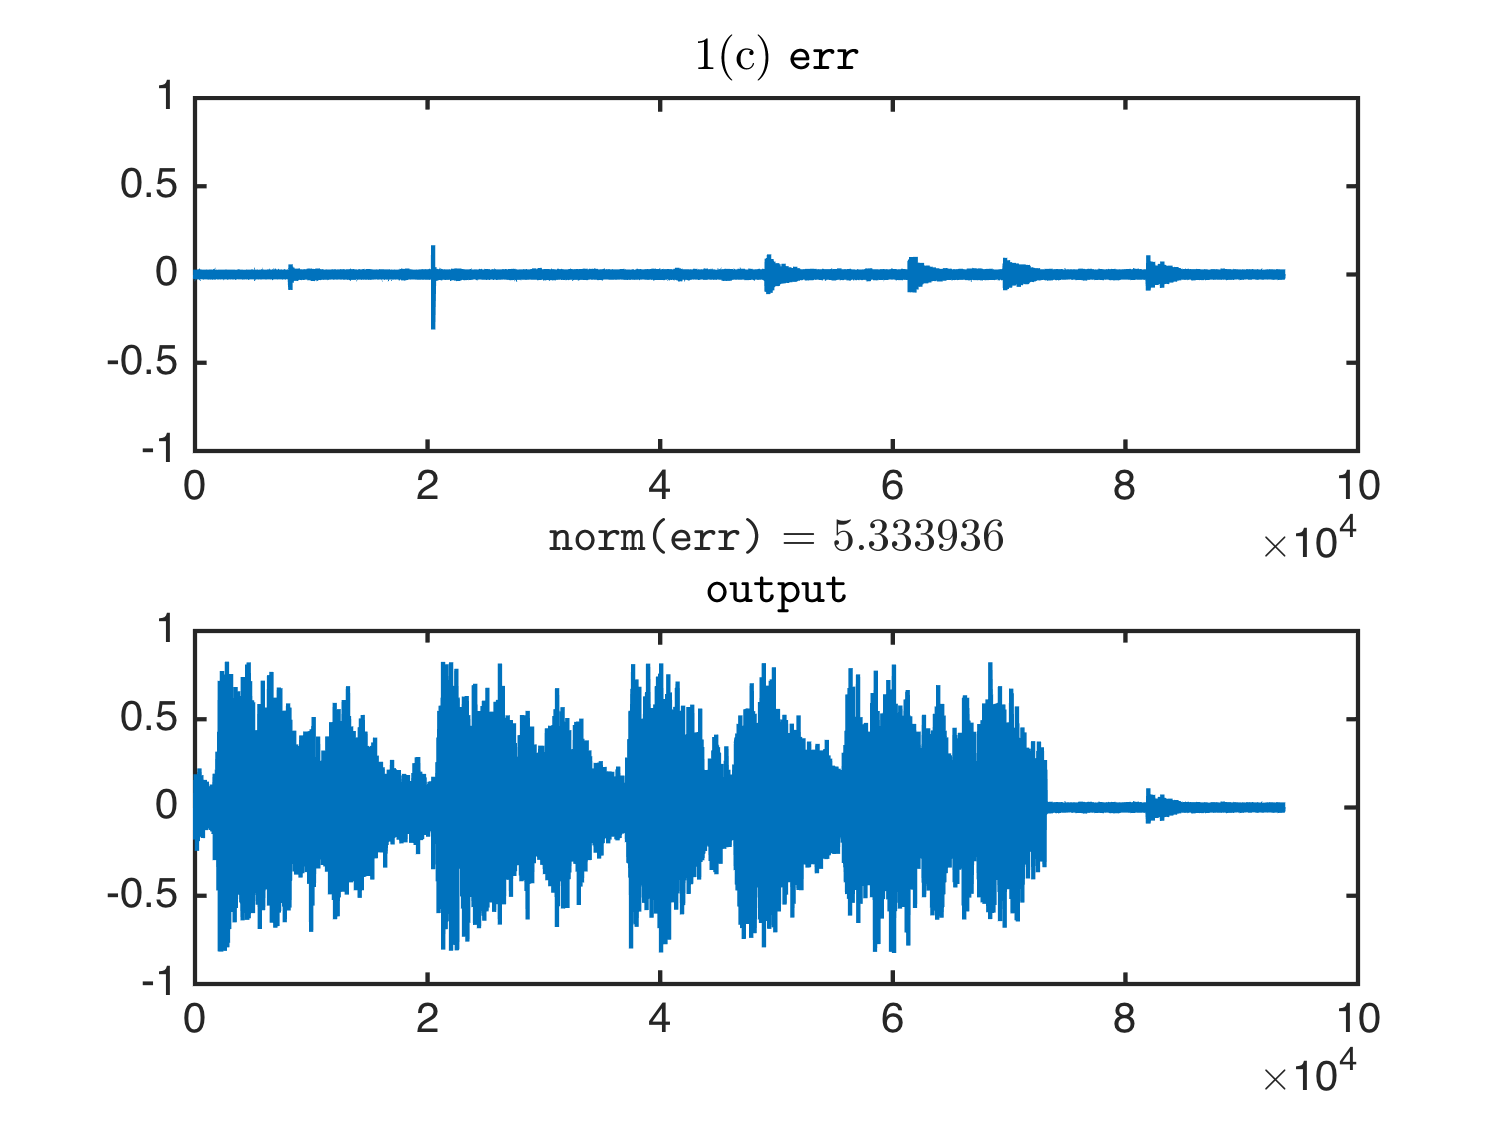
\includegraphics[width=2.5in]{c-rls-output-noisy}
\caption{output and comparison}
\label{c-rls-output-noisy}
\end{minipage}
\end{figure}

In Fig. \ref{c-rls-theta-noisy}, $\theta_9$ and $\theta_{26}$ eventually converge to 0.580 and 0.302. In Fig. \ref{c-rls-output-noisy}, echoes are successfully suppressed and \texttt{err} is negligible comparing with \texttt{noisymike2}.

%--------------------------------------------
%--------------------------------------------

\subsection*{LMS}

\subsubsection*{Noise-free environment}

By trial and error, we find when \texttt{step\_size} = 2$\mu$ = 0.3, the LMS filter has best echo-cancellation performance.
\begin{center}
\texttt{norm(err)} = 1.113590
\end{center}

\begin{figure}[H]
\begin{minipage}[t]{0.33\linewidth}
\centering
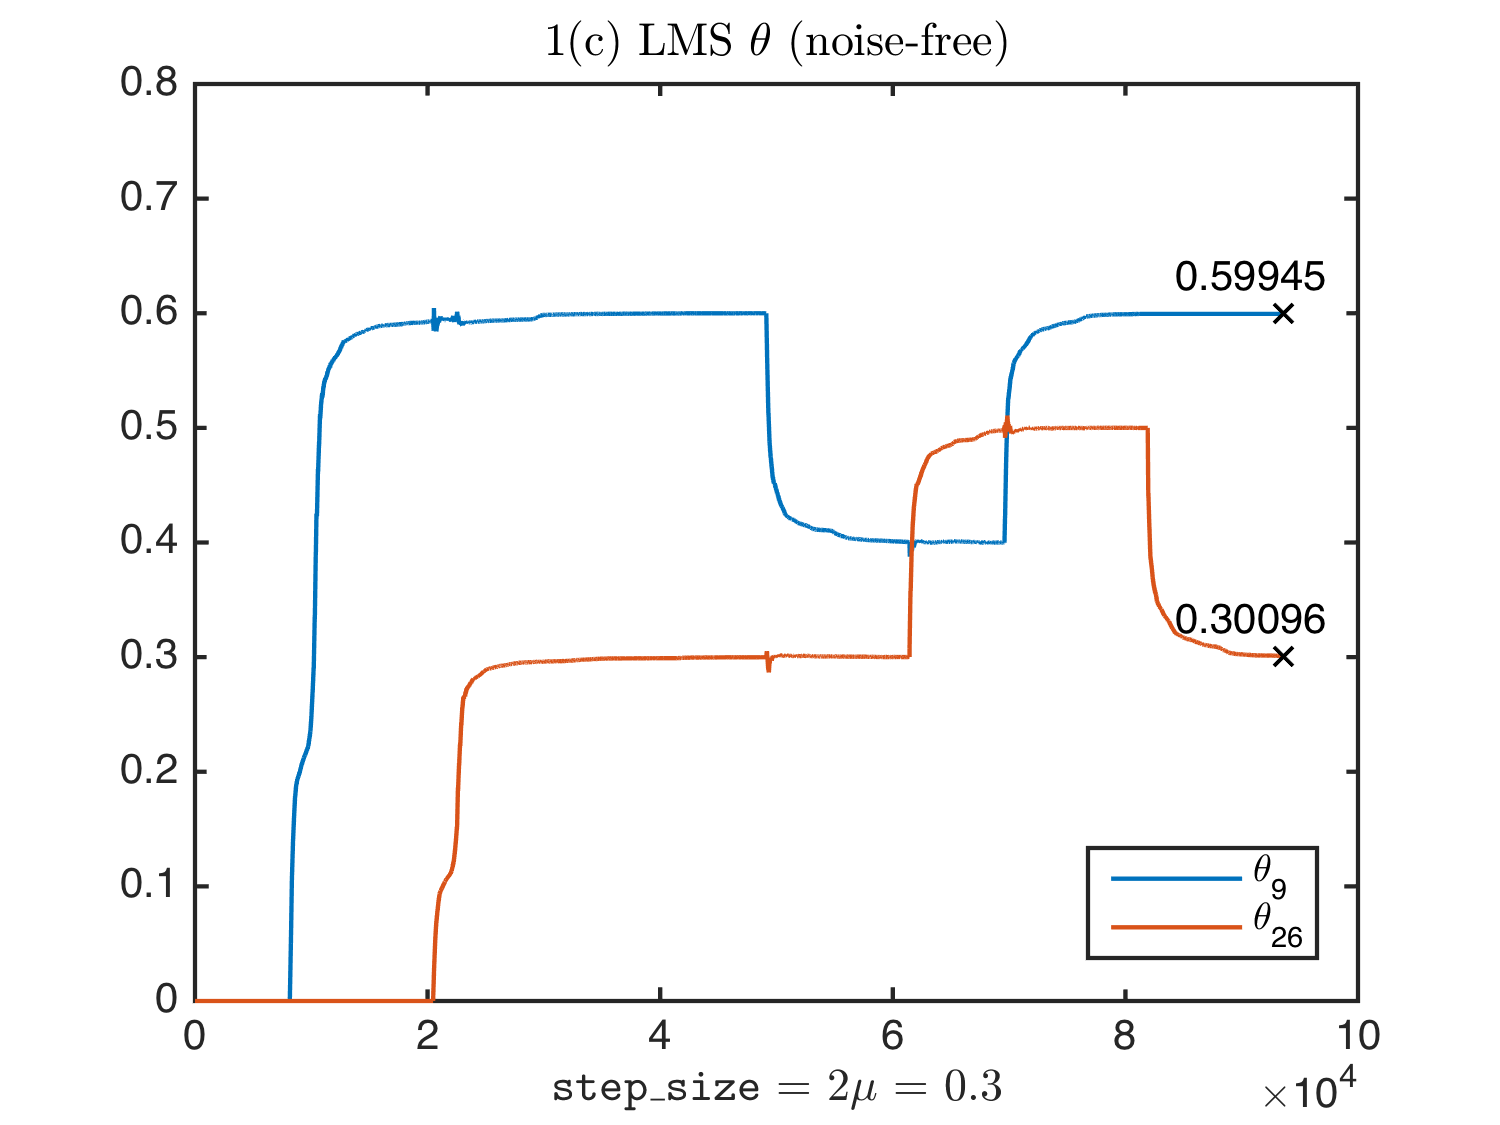
\includegraphics[width=2.5in]{c-lms-theta-noise-free}
\caption{LMS $\theta$ trends}
\label{c-lms-theta-noise-free}
\end{minipage}
\begin{minipage}[t]{0.33\linewidth}
\centering
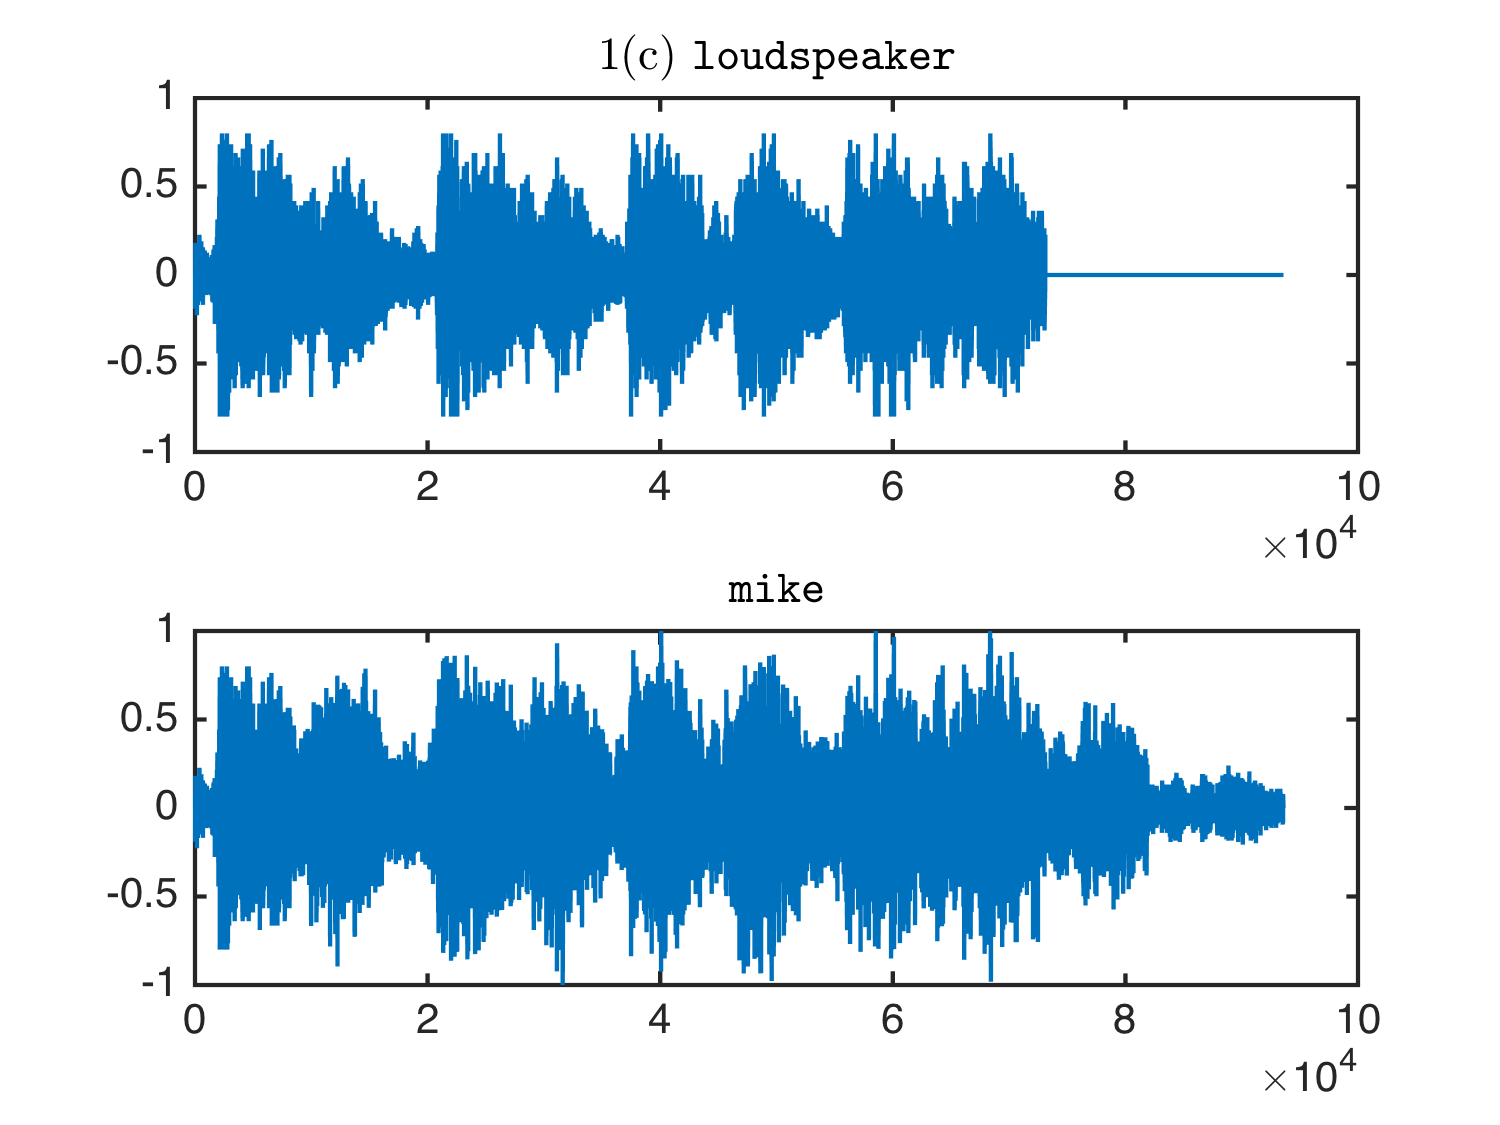
\includegraphics[width=2.5in]{c-lms-input-noise-free}
\caption{inputs}
\end{minipage}
\begin{minipage}[t]{0.33\linewidth}
\centering
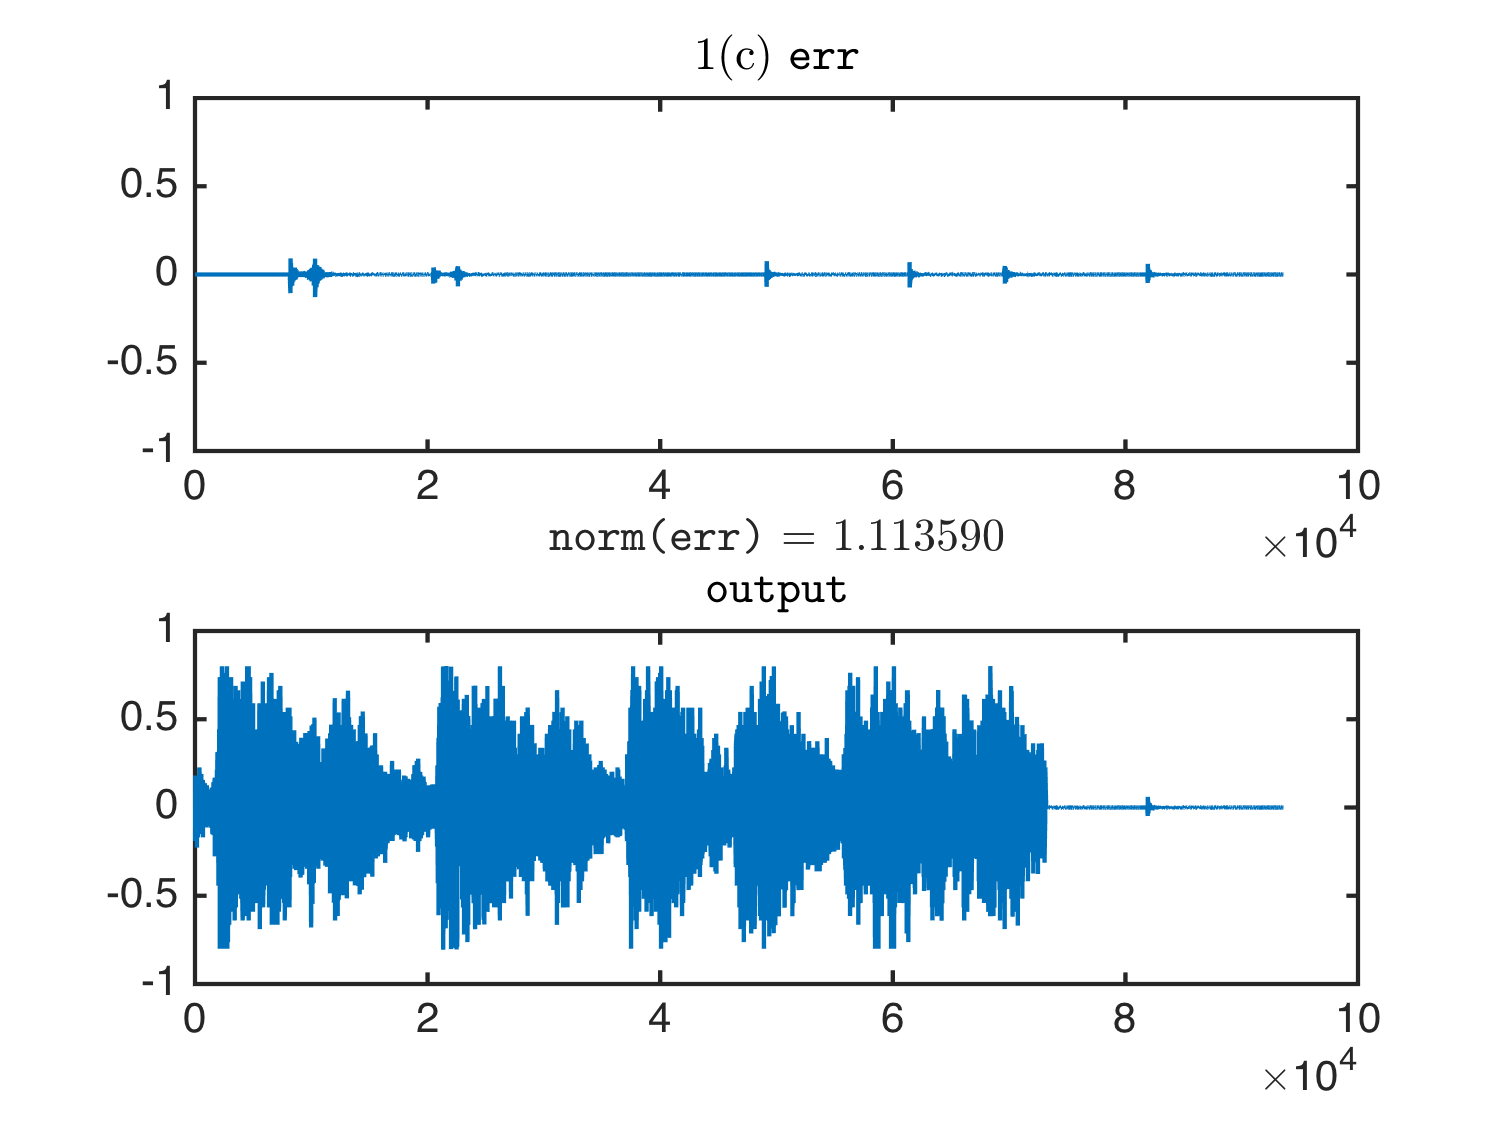
\includegraphics[width=2.5in]{c-lms-output-noise-free}
\caption{output and comparison}
\label{c-lms-output-noise-free}
\end{minipage}
\end{figure}

In Fig. \ref{c-lms-theta-noise-free}, $\theta_9$ and $\theta_{26}$ eventually converge to 0.599 and 0.301. In Fig. \ref{c-lms-output-noise-free}, echoes are successfully suppressed and \texttt{err} is negligible comparing with \texttt{mike2}.

%--------------------------------------------

\subsubsection*{Noisy environment}

By trial and error, we find when \texttt{step\_size} = 2$\mu$ = 0.1, the LMS filter has best echo-cancellation performance.
\begin{center}
\texttt{norm(err)} = 5.294403 $>$ 1.113590
\end{center}
\texttt{norm(err)} increases due to the interference of the background noise.

\begin{figure}[H]
\begin{minipage}[t]{0.33\linewidth}
\centering
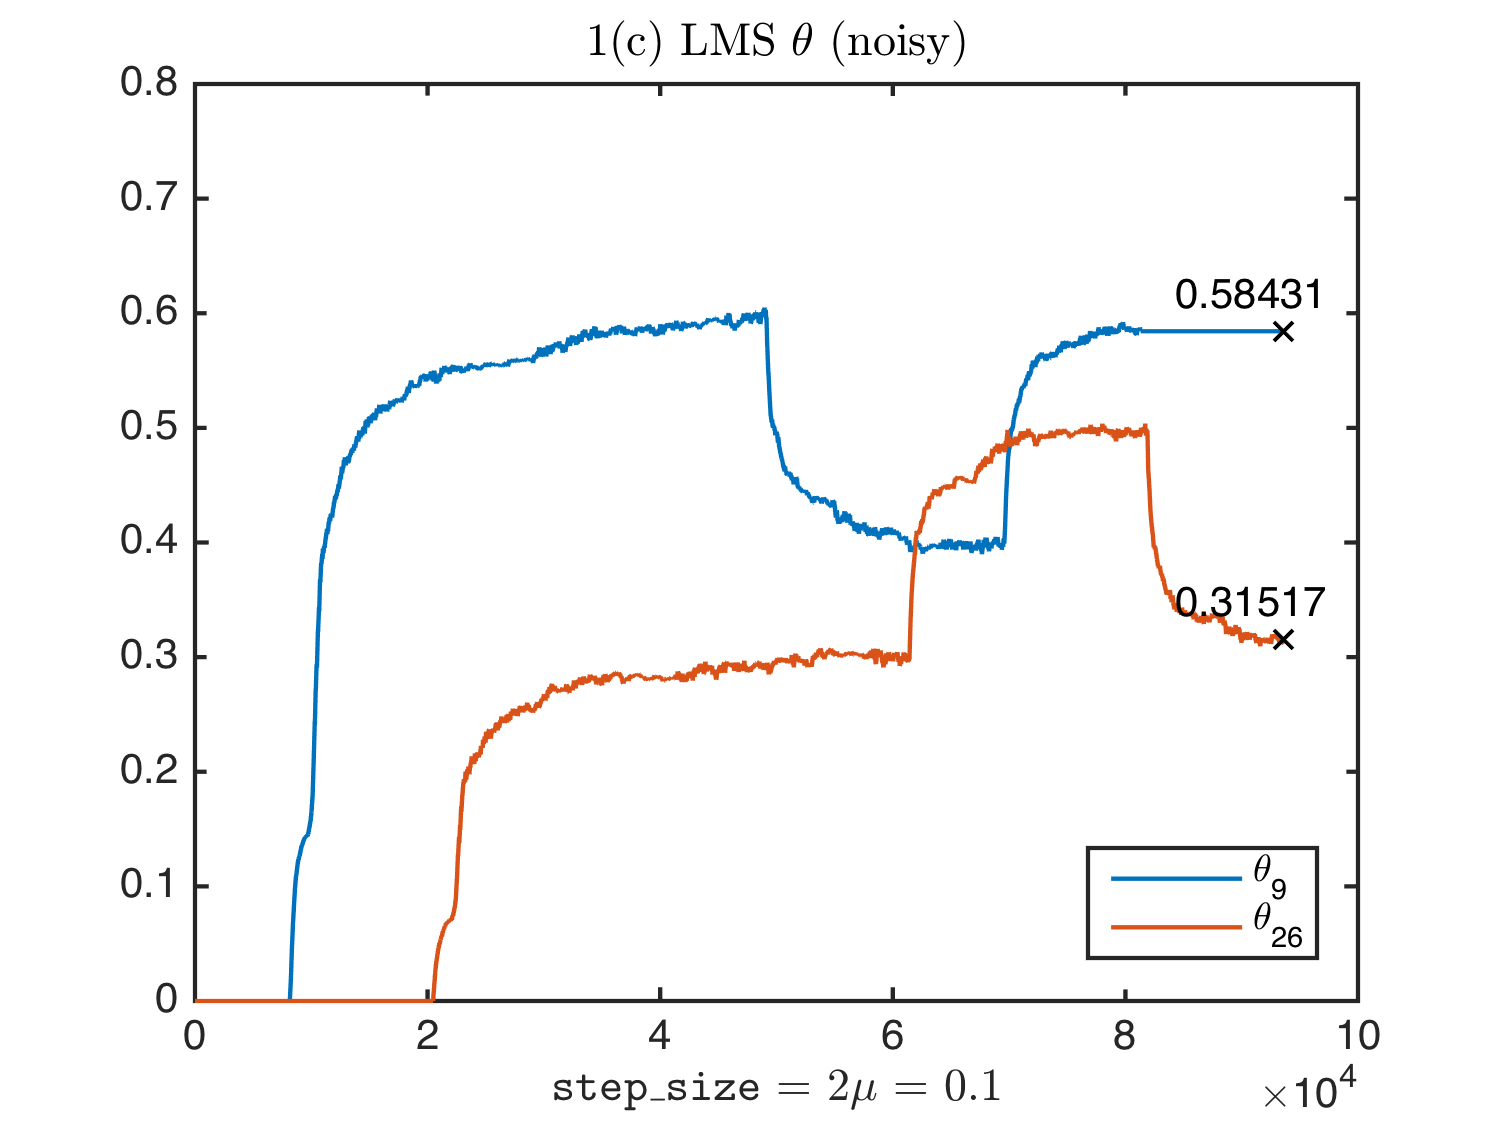
\includegraphics[width=2.5in]{c-lms-theta-noisy}
\caption{LMS $\theta$ trends}
\label{c-lms-theta-noisy}
\end{minipage}
\begin{minipage}[t]{0.33\linewidth}
\centering
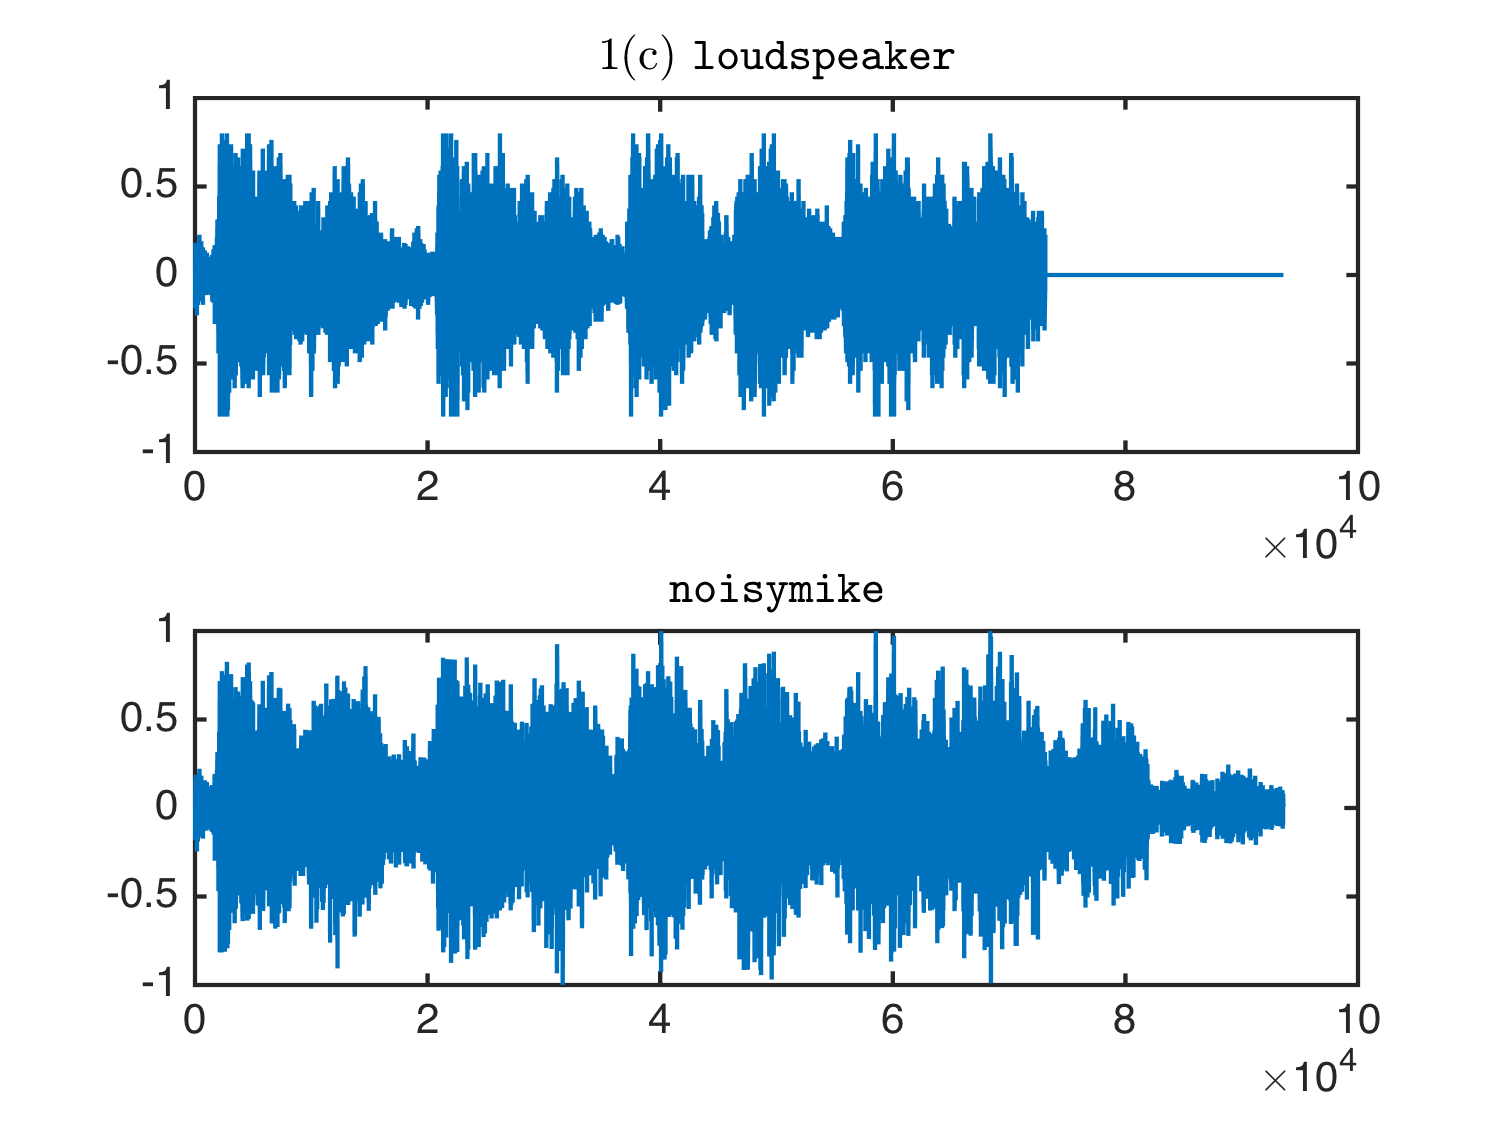
\includegraphics[width=2.5in]{c-lms-input-noisy}
\caption{inputs}
\end{minipage}
\begin{minipage}[t]{0.33\linewidth}
\centering
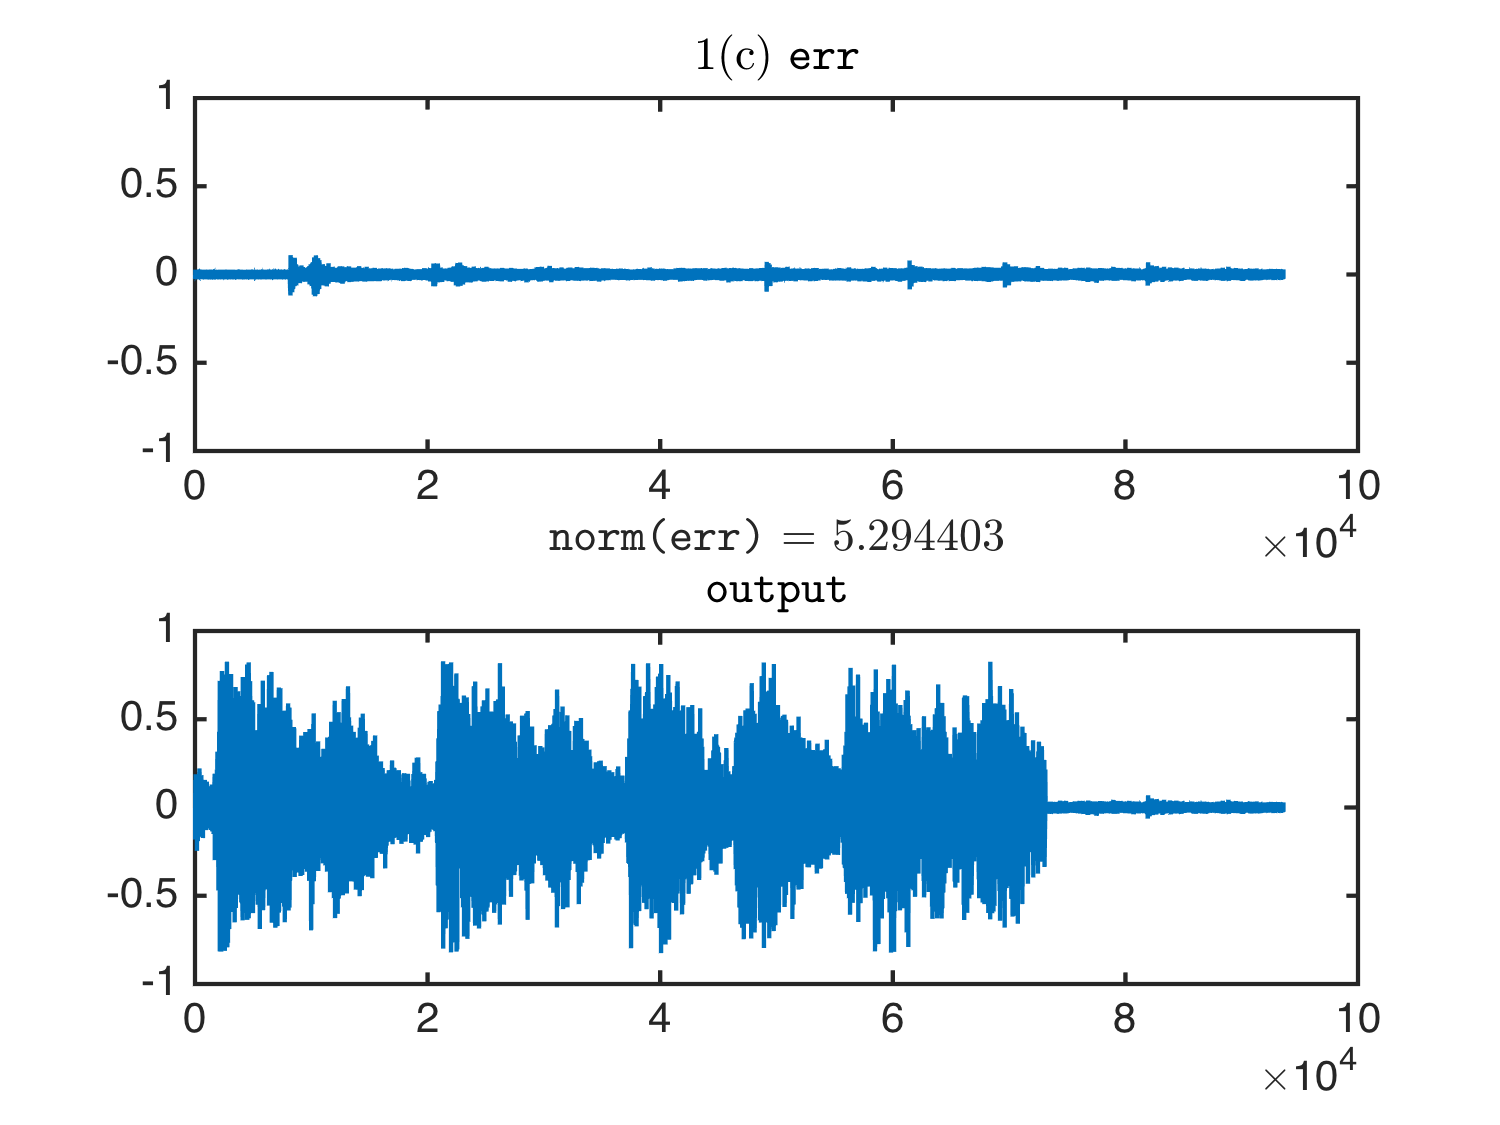
\includegraphics[width=2.5in]{c-lms-output-noisy}
\caption{output and comparison}
\label{c-lms-output-noisy}
\end{minipage}
\end{figure}

In Fig. \ref{c-lms-theta-noisy}, $\theta_9$ and $\theta_{26}$ eventually converge to 0.584 and 0.315. In Fig. \ref{c-lms-output-noisy}, echoes are successfully suppressed and \texttt{err} is negligible comparing with \texttt{noisymike2}.

%----------------------------------------------------------------------------------------
%	Task 1 (d)
%----------------------------------------------------------------------------------------

\section*{Task 1 (d)}

\subsection*{RLS}

\subsubsection*{Noise-free environment}

By trial and error, we find when $\lambda = 1$, $\rho = 3$, the RLS filter has best echo-cancellation performance.
\begin{center}
\texttt{norm(output - loudspeaker)} = 3.084252
\end{center}

\begin{figure}[H]
\begin{minipage}[t]{0.33\linewidth}
\centering
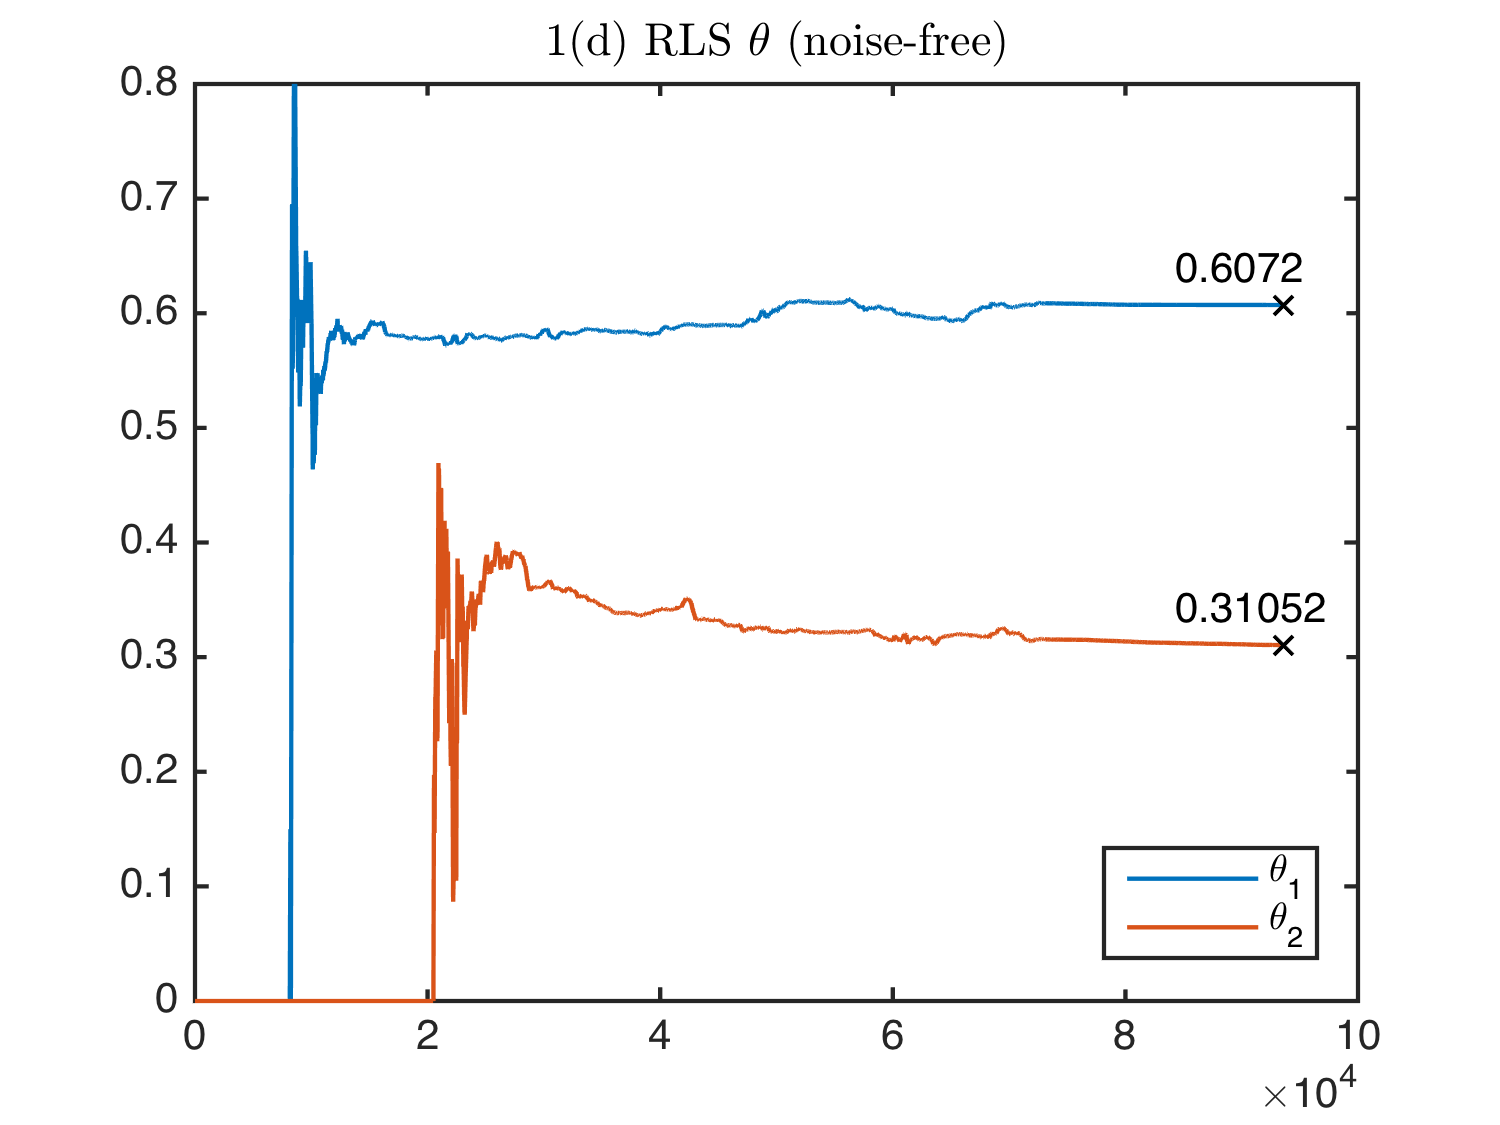
\includegraphics[width=2.5in]{d-rls-theta-noise-free}
\caption{RLS $\theta$ trends}
\label{d-rls-theta-noise-free}
\end{minipage}
\begin{minipage}[t]{0.33\linewidth}
\centering
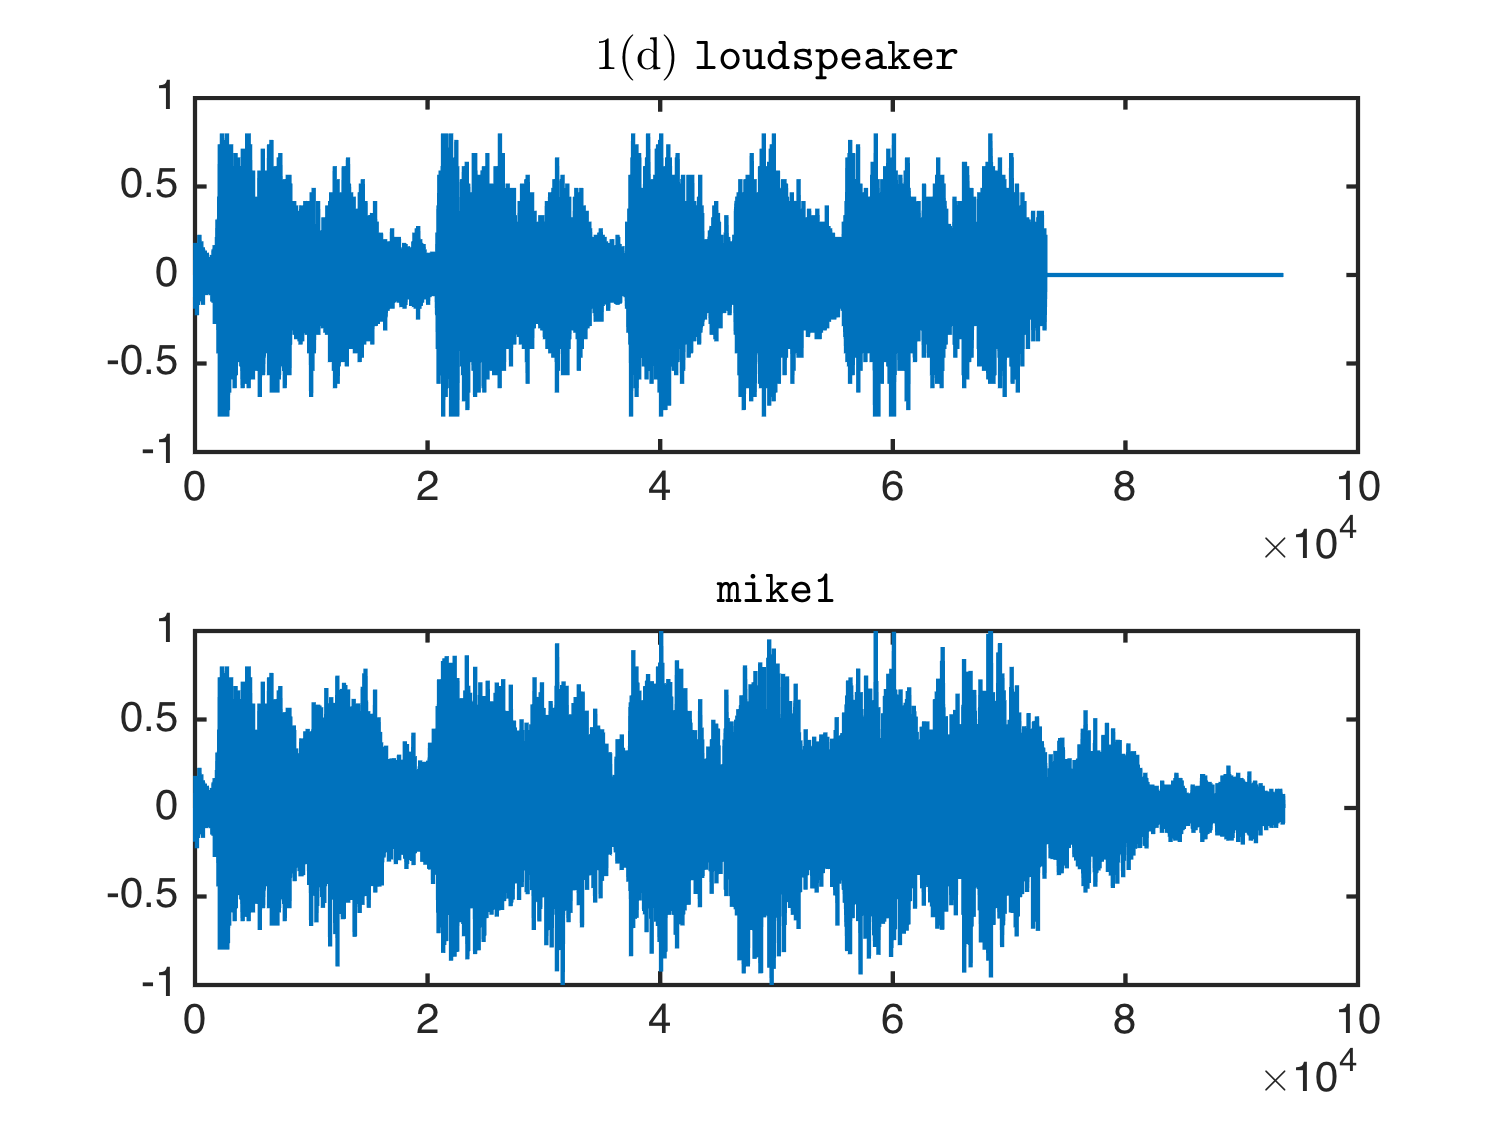
\includegraphics[width=2.5in]{d-rls-input-noise-free}
\caption{inputs}
\end{minipage}
\begin{minipage}[t]{0.33\linewidth}
\centering
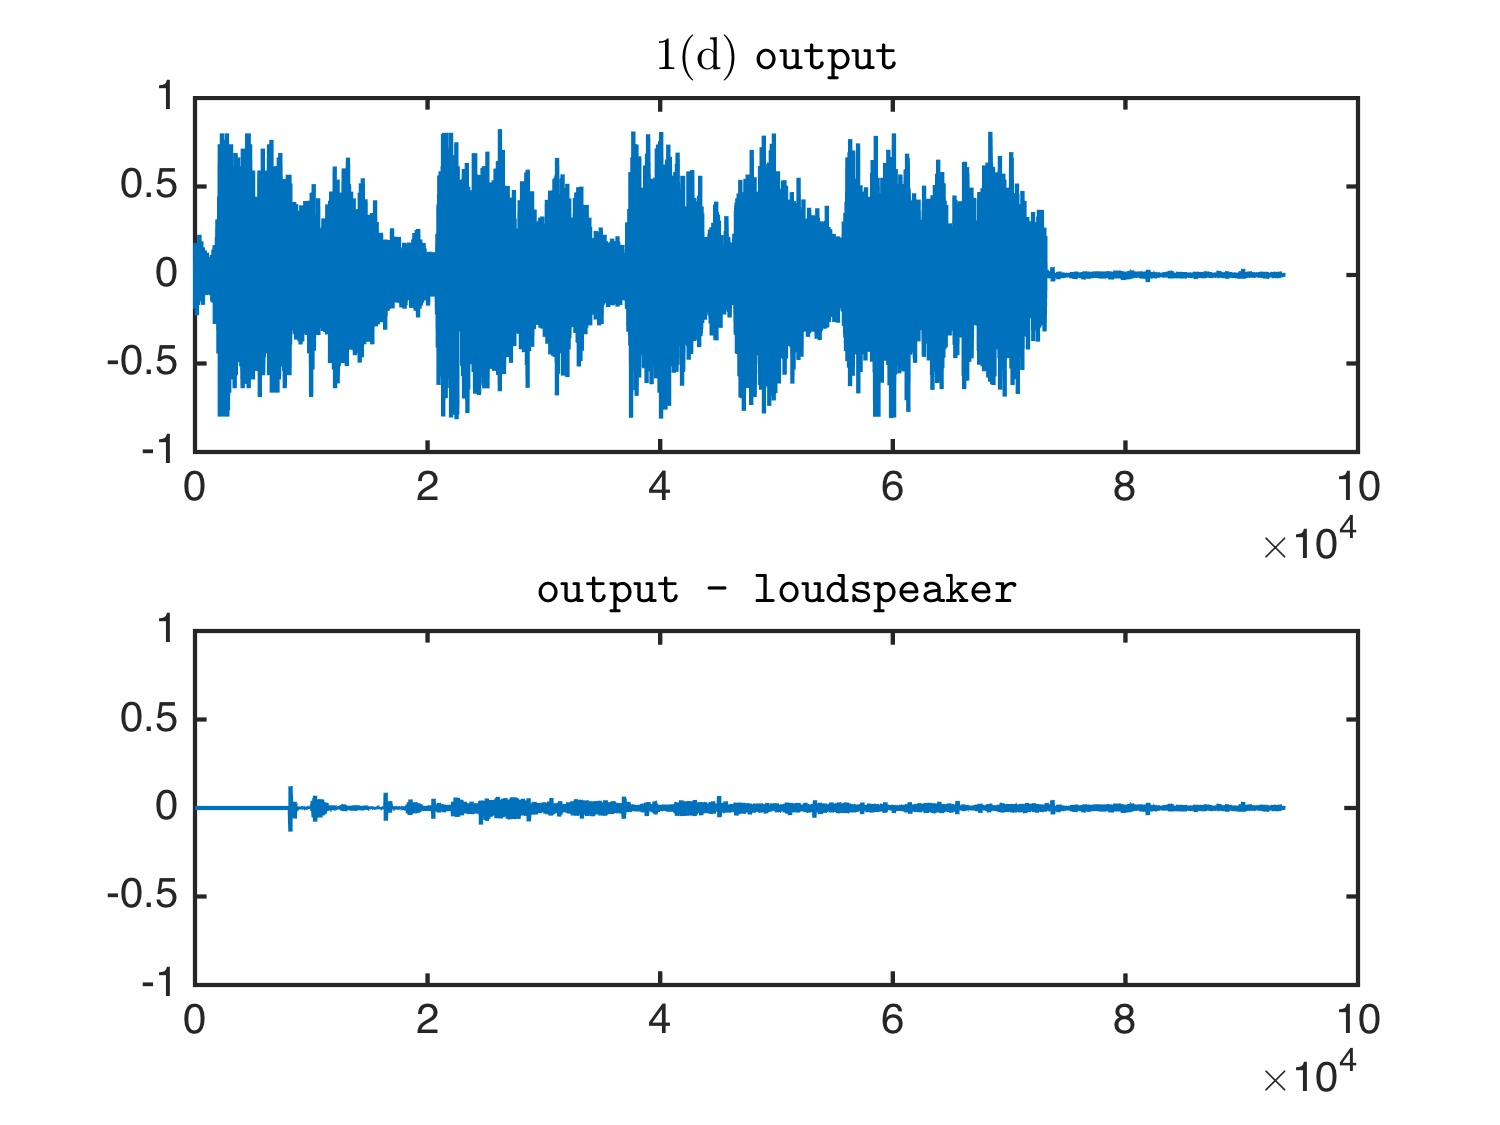
\includegraphics[width=2.5in]{d-rls-output-noise-free}
\caption{output and comparison}
\label{d-rls-output-noise-free}
\end{minipage}
\end{figure}

In Fig. \ref{d-rls-theta-noise-free}, $\theta_1$ and $\theta_2$ eventually converge. In Fig. \ref{d-rls-output-noise-free}, echoes are successfully suppressed and \texttt{output - loudspeaker} is negligible comparing with \texttt{mike1}.

%--------------------------------------------

\subsubsection*{Noisy environment}

By trial and error, we find when $\lambda = 1$, $\rho = 3$, the RLS filter has best echo-cancellation performance.
\begin{center}
\texttt{norm(output - loudspeaker)} = 7.224809 $>$ 3.084252
\end{center}
\texttt{norm(output - loudspeaker)} increases due to the interference of the background noise.

\begin{figure}[H]
\begin{minipage}[t]{0.33\linewidth}
\centering
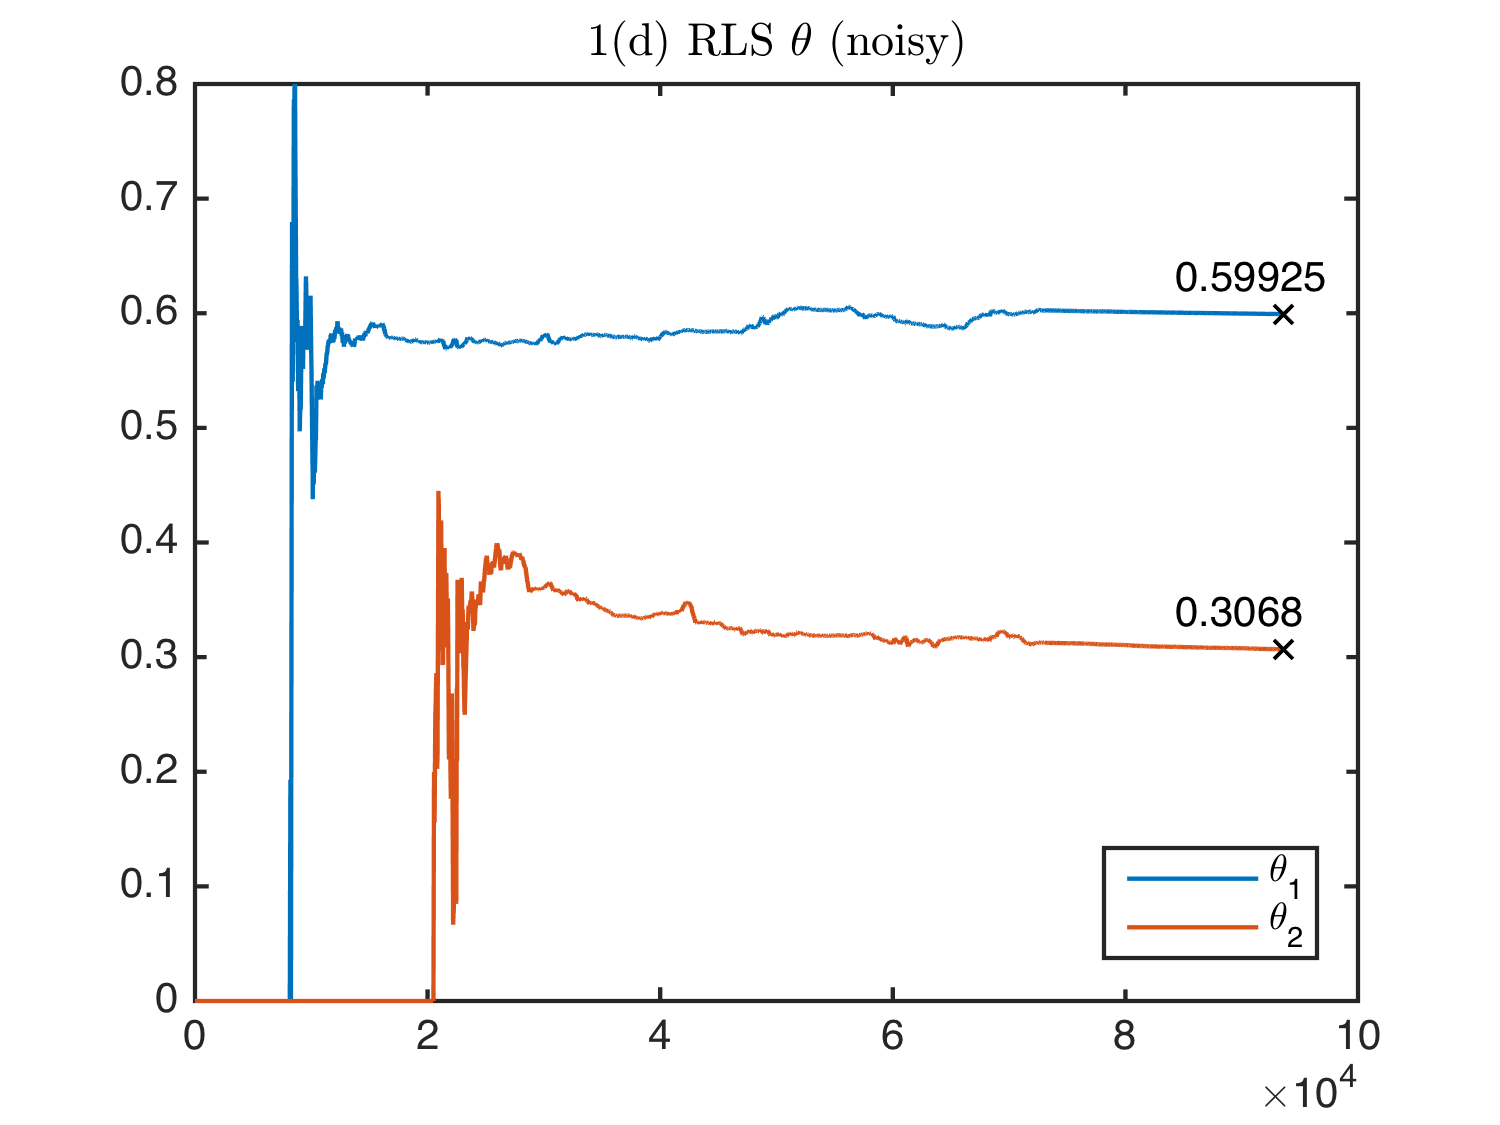
\includegraphics[width=2.5in]{d-rls-theta-noisy}
\caption{RLS $\theta$ trends}
\label{d-rls-theta-noisy}
\end{minipage}
\begin{minipage}[t]{0.33\linewidth}
\centering
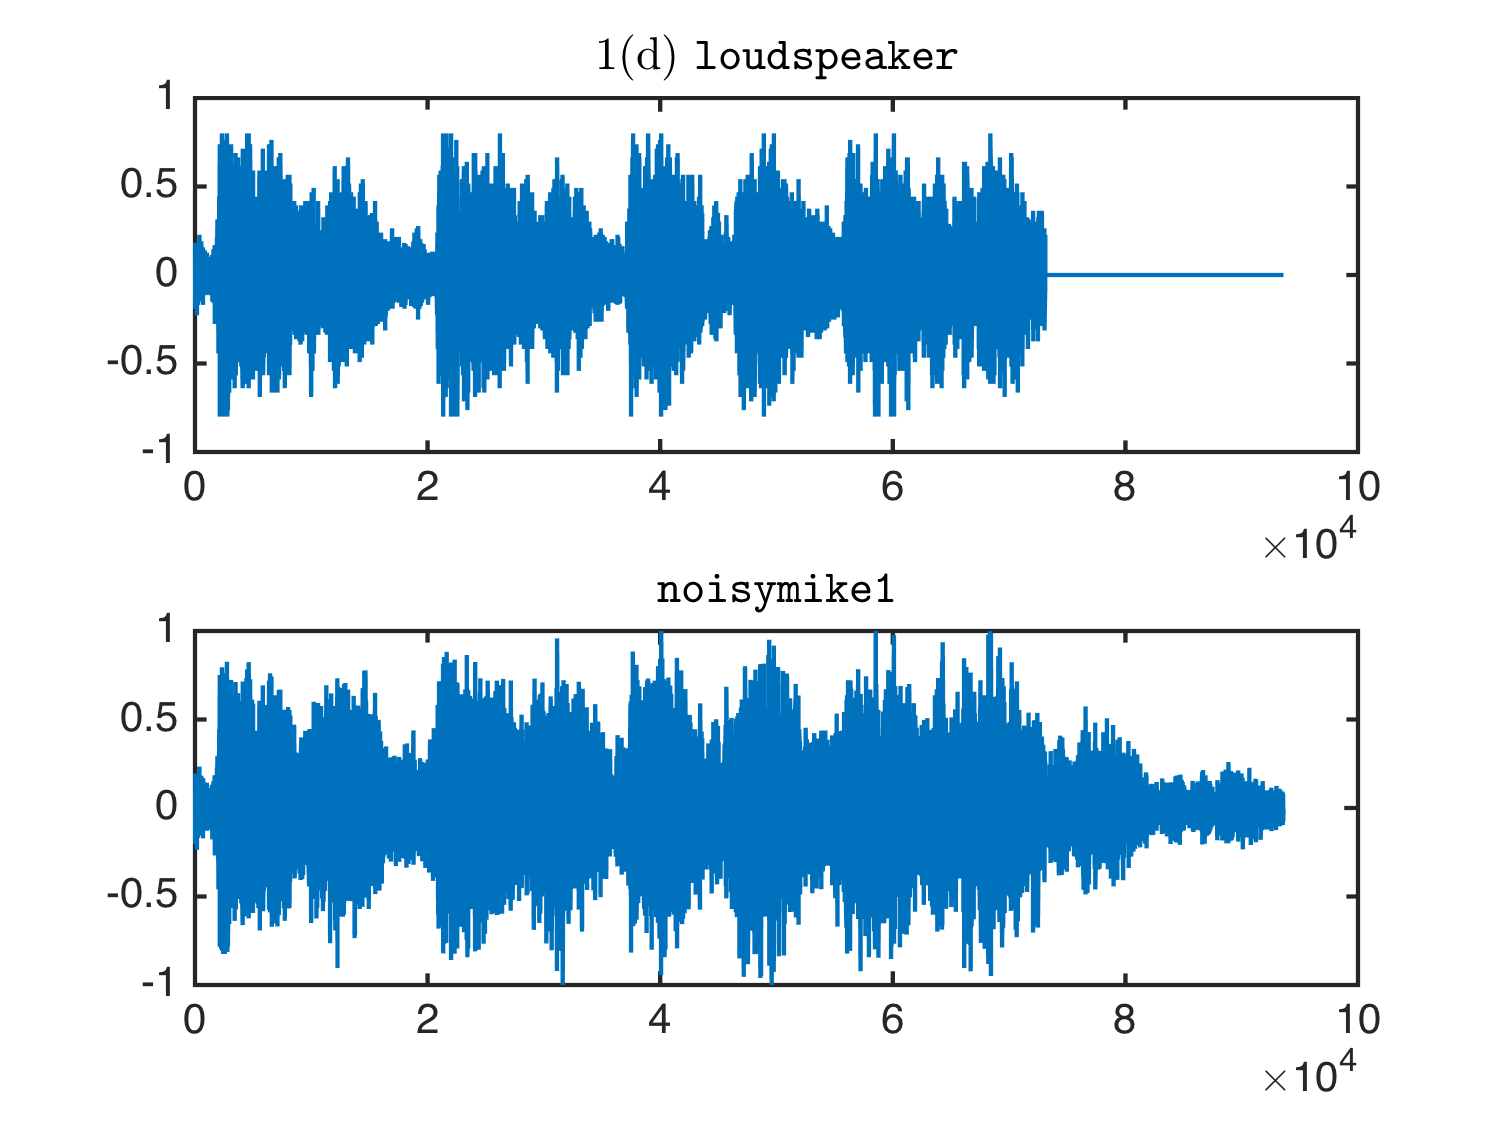
\includegraphics[width=2.5in]{d-rls-input-noisy}
\caption{inputs}
\end{minipage}
\begin{minipage}[t]{0.33\linewidth}
\centering
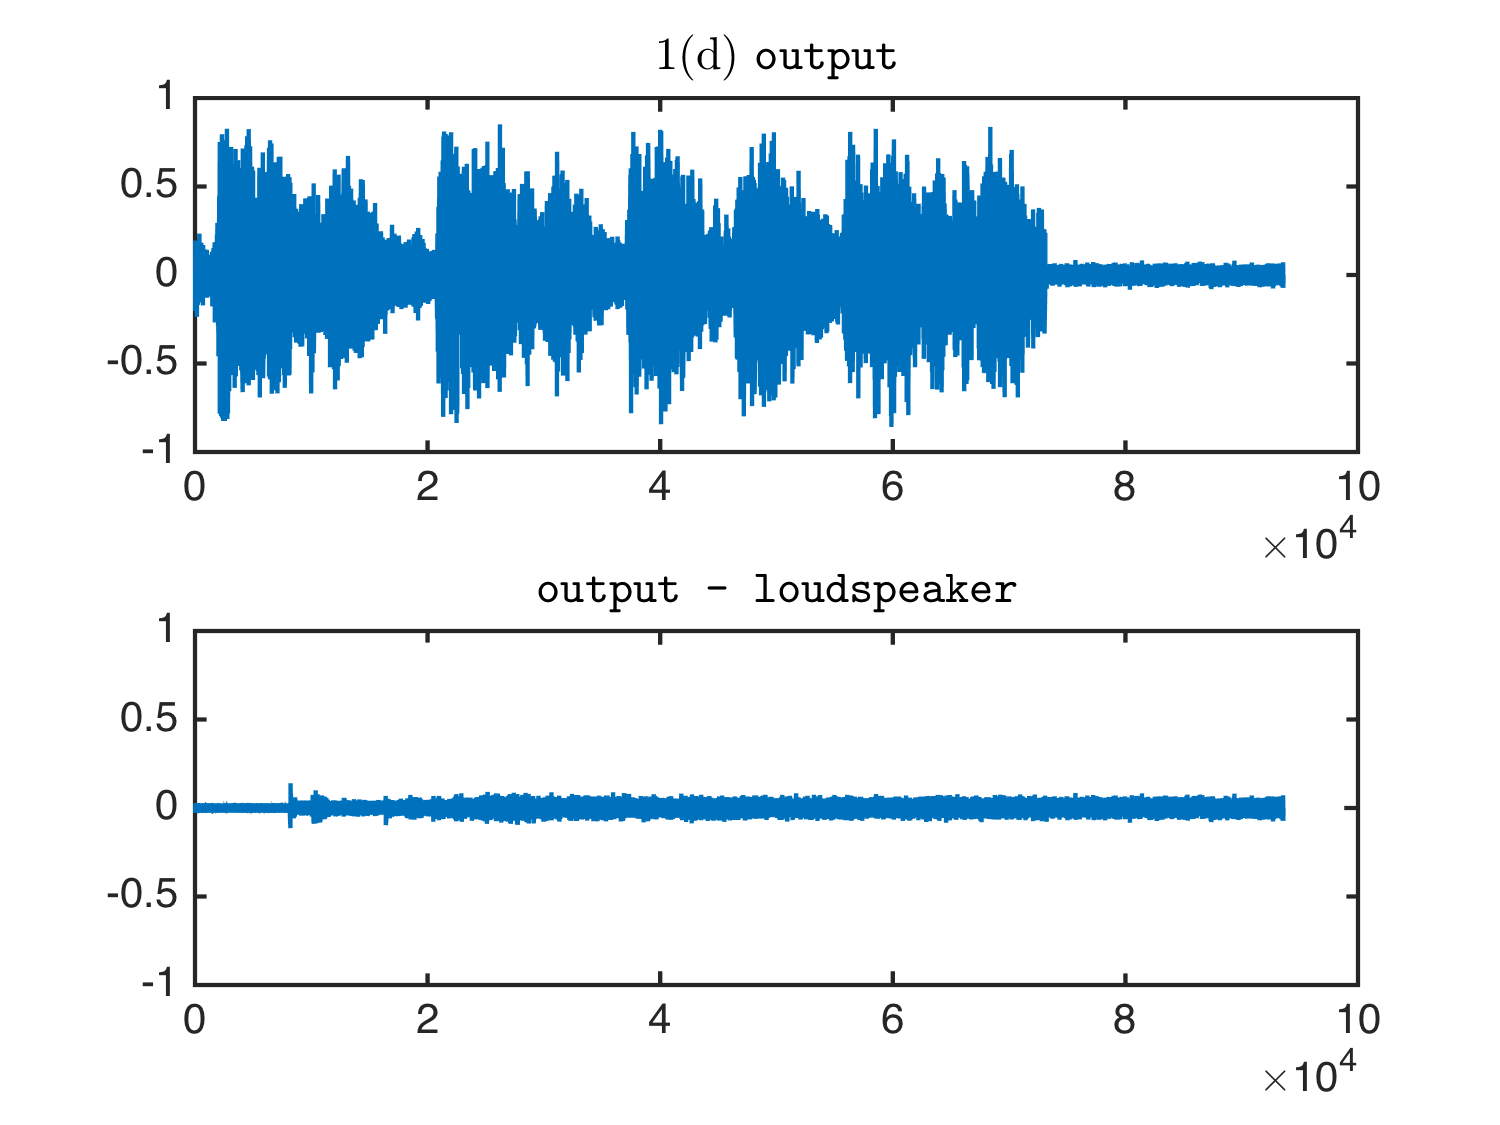
\includegraphics[width=2.5in]{d-rls-output-noisy}
\caption{output and comparison}
\label{d-rls-output-noisy}
\end{minipage}
\end{figure}

In Fig. \ref{d-rls-theta-noisy}, $\theta_1$ and $\theta_2$ eventually converge. In Fig. \ref{d-rls-output-noisy}, echoes are successfully suppressed and \texttt{output - loudspeaker} is negligible comparing with \texttt{noisymike1}.

%--------------------------------------------
%--------------------------------------------

\subsection*{LMS}

\subsubsection*{Noise-free environment}

By trial and error, we find when \texttt{step\_size} = 2$\mu$ = 0.015, the LMS filter has best echo-cancellation performance.
\begin{center}
\texttt{norm(output - loudspeaker)} = 8.113330
\end{center}

\begin{figure}[H]
\begin{minipage}[t]{0.33\linewidth}
\centering
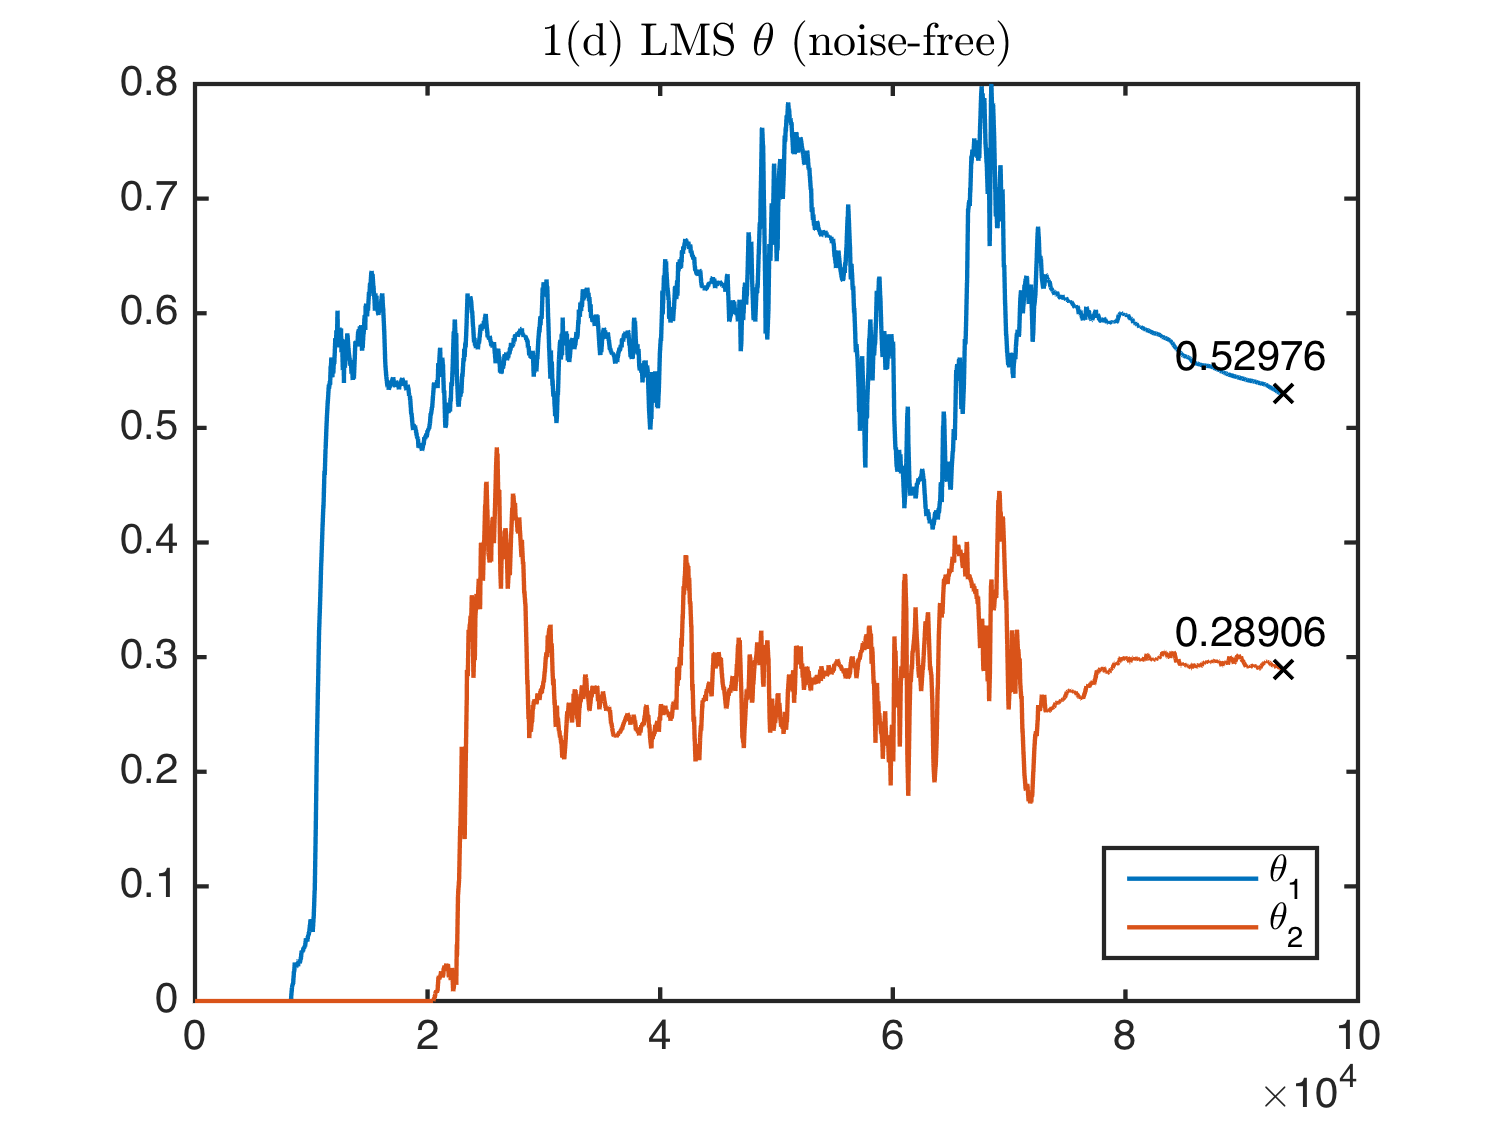
\includegraphics[width=2.5in]{d-lms-theta-noise-free}
\caption{LMS $\theta$ trends}
\label{d-lms-theta-noise-free}
\end{minipage}
\begin{minipage}[t]{0.33\linewidth}
\centering
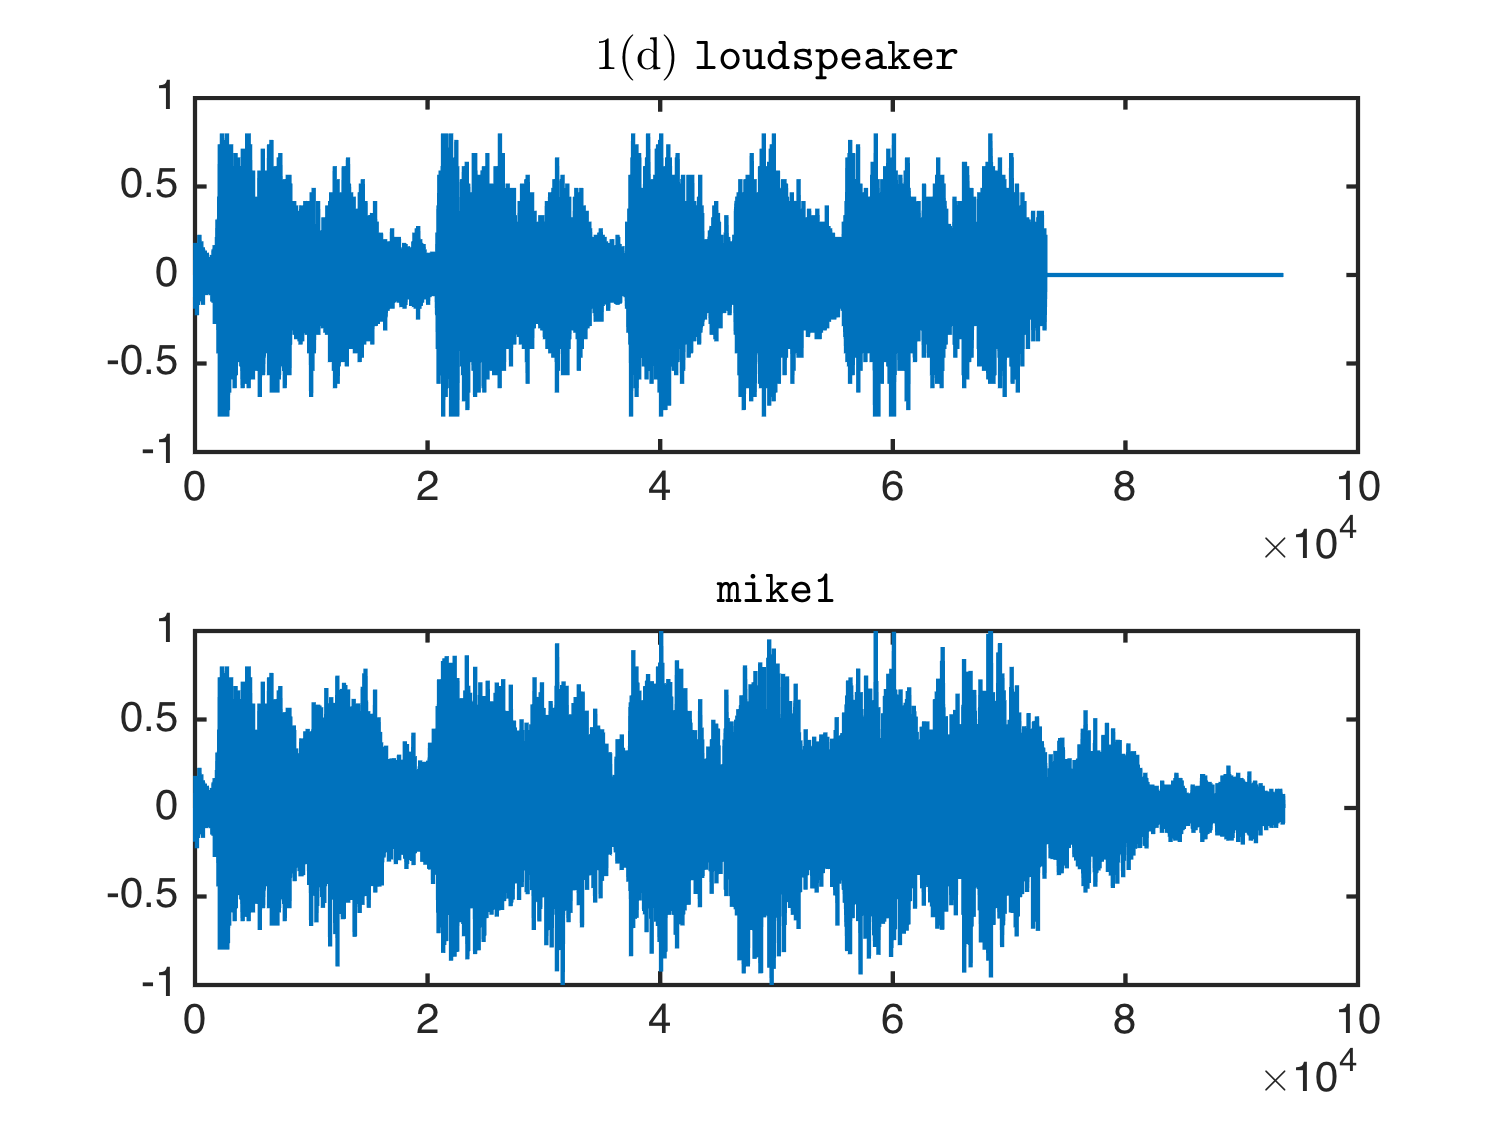
\includegraphics[width=2.5in]{d-lms-input-noise-free}
\caption{inputs}
\end{minipage}
\begin{minipage}[t]{0.33\linewidth}
\centering
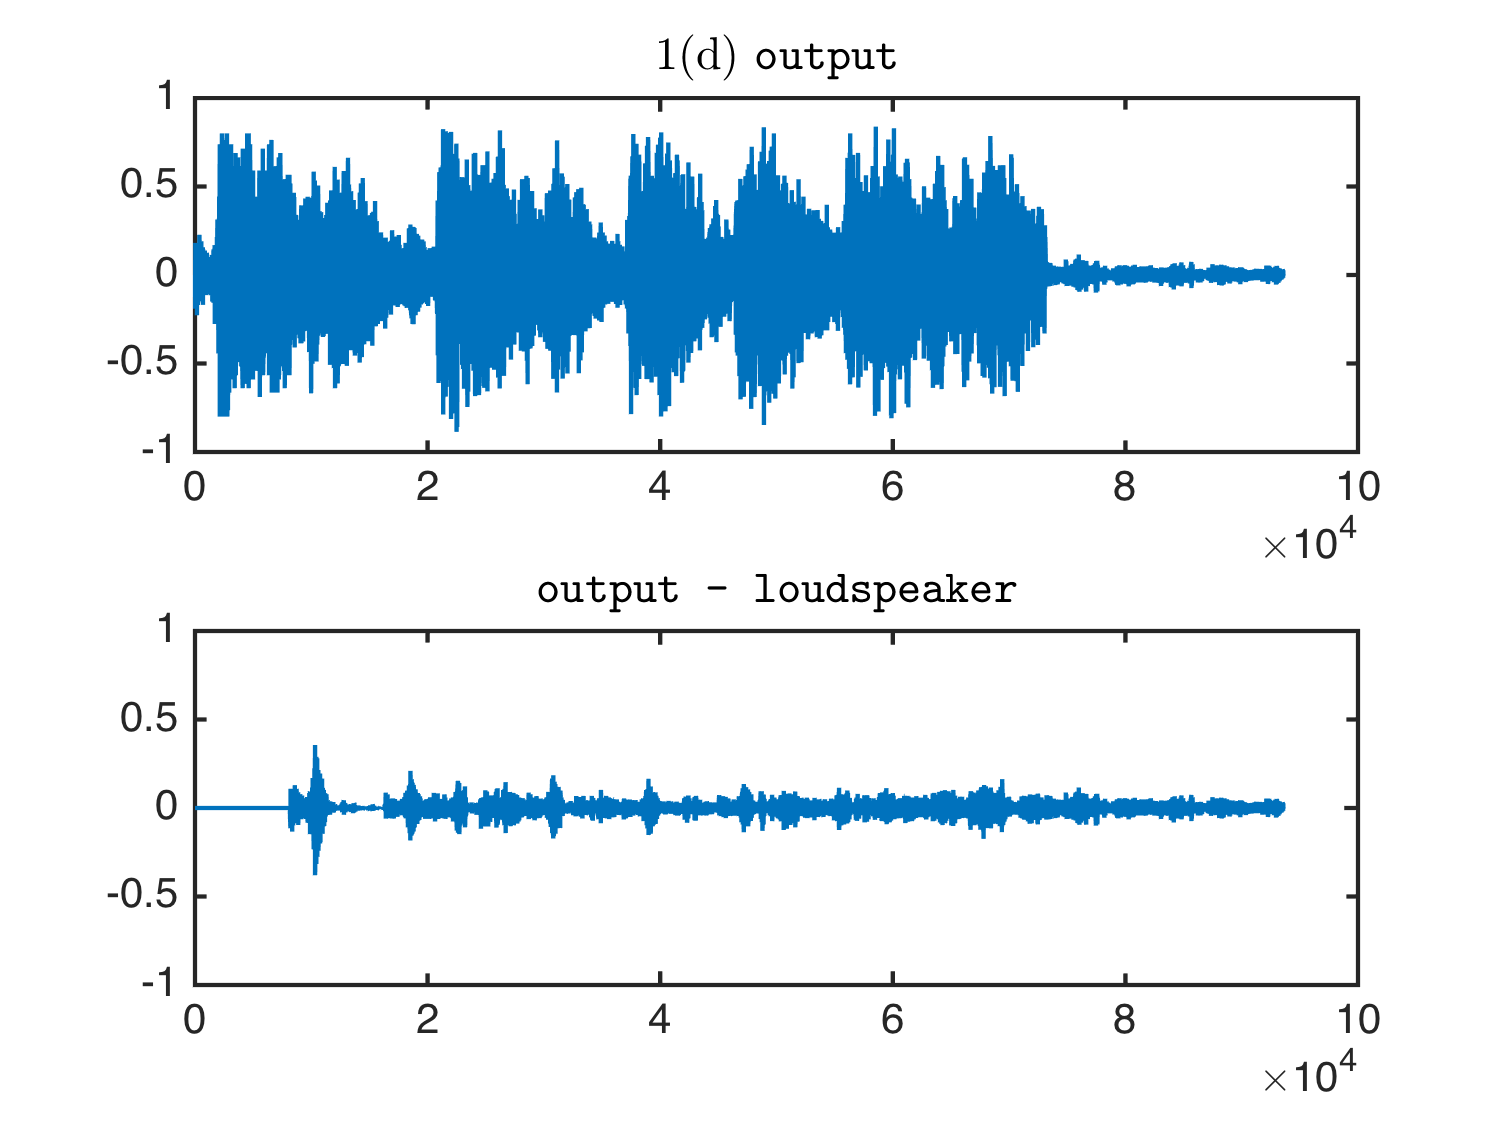
\includegraphics[width=2.5in]{d-lms-output-noise-free}
\caption{output and comparison}
\label{d-lms-output-noise-free}
\end{minipage}
\end{figure}

In Fig. \ref{d-lms-theta-noise-free}, $\theta_1$ and $\theta_2$ eventually converge. In Fig. \ref{d-lms-output-noise-free}, echoes are successfully suppressed and \texttt{output - loudspeaker} is negligible comparing with \texttt{mike1}.

%--------------------------------------------

\subsubsection*{Noisy environment}

By trial and error, we find when \texttt{step\_size} = 2$\mu$ = 0.015, the LMS filter has best echo-cancellation performance.
\begin{center}
\texttt{norm(output - loudspeaker)} = 10.257979 $>$ 8.113330
\end{center}
\texttt{norm(output - loudspeaker)} increases due to the interference of the background noise.

\begin{figure}[H]
\begin{minipage}[t]{0.33\linewidth}
\centering
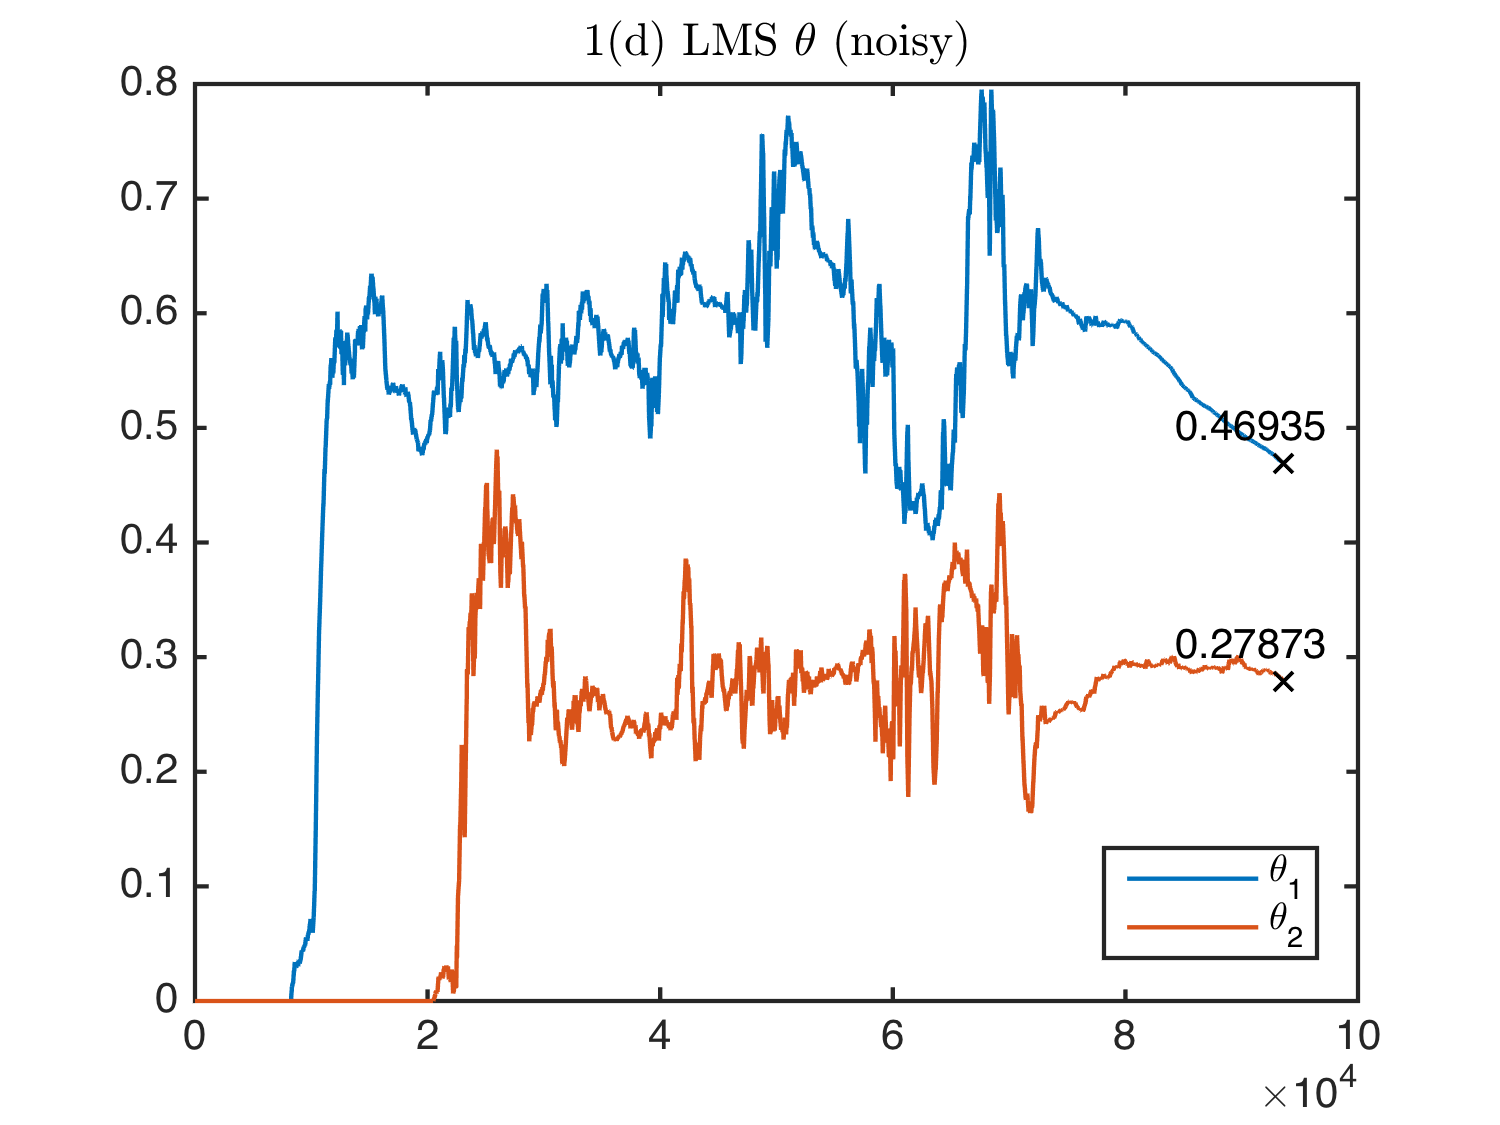
\includegraphics[width=2.5in]{d-lms-theta-noisy}
\caption{LMS $\theta$ trends}
\label{d-lms-theta-noisy}
\end{minipage}
\begin{minipage}[t]{0.33\linewidth}
\centering
\includegraphics[width=2.5in]{d-lms-input-noisy}
\caption{inputs}
\end{minipage}
\begin{minipage}[t]{0.33\linewidth}
\centering
\includegraphics[width=2.5in]{d-lms-output-noisy}
\caption{output and comparison}
\label{d-lms-output-noisy}
\end{minipage}
\end{figure}

In Fig. \ref{d-lms-theta-noisy}, $\theta_1$ and $\theta_2$ eventually converge. In Fig. \ref{d-lms-output-noisy}, echoes are successfully suppressed and \texttt{output - loudspeaker} is negligible comparing with \texttt{noisymike1}.

%----------------------------------------------------------------------------------------
%	Task 2 Prelab
%----------------------------------------------------------------------------------------

\section*{Task 2 Prelab}

\subsection*{LMS}

\begin{align*}
e(N) &= y(N) - \phi(N)^T \hat{\theta}(N-1)\\
\hat{\theta}(N) &= \hat{\theta}(N-1) + 2 \mu \phi(N) e(N)
\end{align*}

\begin{align*}
e(N) &= y(N) - (\phi_1(N) \hat{\theta}_1(N-1) + \phi_2(N) \hat{\theta}_2(N-1))
\end{align*}

\begin{align*}
\begin{bmatrix}
\hat{\theta}_1(N)\\
\hat{\theta}_2(N)
\end{bmatrix}
&=
\begin{bmatrix}
\hat{\theta}_1(N-1)\\
\hat{\theta}_2(N-1)
\end{bmatrix}
+ 2 \mu
\begin{bmatrix}
\phi_1(N)\\
\phi_2(N)
\end{bmatrix}
e(N)\\
&=
\begin{bmatrix}
\hat{\theta}_1(N-1) + 2\mu \phi_1(N) e(N)\\
\hat{\theta}_2(N-1) + 2\mu \phi_2(N) e(N)
\end{bmatrix}
\end{align*}

\subsubsection*{Optimization}
$\mu$ is a constant, $2\mu$ is constant as well. Hence, we consider $2\mu$ together as one floating point number to reduce multiplications. Additionally, $2\mu \cdot e(N)$ can be cached.

\begin{lstlisting}[language={C}]
float err = out - (in1 * gain[0] + in2 * gain[1]);
float factor = 1e-18 * err;
gain[0] += in1 * factor;
gain[1] += in2 * factor;
\end{lstlisting}

\subsection*{RLS}

\begin{align*}
e(N) &= y(N) - \phi(N)^T \hat{\theta}(N-1)\\
P(N) &= \frac{1}{\lambda} \Big( P(N-1) - \frac{P(N-1) \phi(N) \phi(N)^T P(N-1)}{\lambda + \phi(N)^T P(N-1) \phi(N)} \Big)\\
&= \frac{1}{\lambda} \Big( P(N-1) - \frac{NUM}{DEN} \Big)\\
\hat{\theta}(N) &= \hat{\theta}(N-1) + P(N) \phi(N) e(N)
\end{align*}

\begin{align*}
\phi &=
\begin{bmatrix}
in1\\
in2
\end{bmatrix}
&\hat{\theta} &=
\begin{bmatrix}
gain0\\
gain1
\end{bmatrix}
&P &=
\begin{bmatrix}
P11 & P12\\
P21 & P22
\end{bmatrix}
\end{align*}

\begin{align*}
err &= out - (in1 * gain0 + in2 * gain1)
\end{align*}

\begin{align*}
DEN &= lambda + in1*(P11*in1 + P21*in2) + in2*(P12*in1 + P22*in2)\\
NUM11 &= P11*in1*(P11*in1 + P12*in2) + P21*in2*(P11*in1 + P12*in2)\\
NUM12 &= P12*in1*(P11*in1 + P12*in2) + P22*in2*(P11*in1 + P12*in2)\\
NUM21 &= P11*in1*(P21*in1 + P22*in2) + P21*in2*(P21*in1 + P22*in2)\\
NUM22 &= P12*in1*(P21*in1 + P22*in2) + P22*in2*(P21*in1 + P22*in2)
\end{align*}

\begin{align*}
\begin{bmatrix}
P11 & P12\\
P21 & P22
\end{bmatrix}
= \frac{1}{lambda}
\Big(
\begin{bmatrix}
P11 & P12\\
P21 & P22
\end{bmatrix}
- \frac{1}{DEN}
\begin{bmatrix}
NUM11 & NUM12\\
NUM21 & NUM22
\end{bmatrix}
\Big)
\end{align*}

\begin{align*}
\begin{bmatrix}
gain0\\
gain1
\end{bmatrix}
=
\begin{bmatrix}
gain0 + err * (P11*in1 + P12*in2)\\
gain1 + err * (P21*in1 + P22*in2)
\end{bmatrix}
\end{align*}

\textit{Most of the preceding calculations are done in MATLAB by creating symbolic variables. The code can be found in the appendix on page \pageref{rls_syms}.}

\subsubsection*{Optimization}
RLS algorithm is much more time-consuming than LMS. We optimize in the following ways.\\

Firstly, we cache multiplications in \texttt{v1} to \texttt{v6}. Secondly, we precompute the reciprocal of $\lambda$ in MATLAB because floating point multiplication is faster than division. The reciprocal of $DEN$ is also precomputed and cached.

\begin{lstlisting}[language={C}]
float lambda = 0.98;
float lambda_reciprocal = 1.020408163;

float v1 = P11*in1;
float v2 = P12*in1;
float v3 = P12*in2;
float v4 = P21*in1;
float v5 = P21*in2;
float v6 = P22*in2;

float den_reciprocal = 1 / ( lambda + in1*(v1 + v5) + in2*(v2 + v6) );

P11 = (P11 - (v1*(v1 + v3) + v5*(v1 + v3)) * den_reciprocal) * lambda_reciprocal;
P12 = (P12 - (v2*(v1 + v3) + v6*(v1 + v3)) * den_reciprocal) * lambda_reciprocal;
P21 = (P21 - (v1*(v4 + v6) + v5*(v4 + v6)) * den_reciprocal) * lambda_reciprocal;
P22 = (P22 - (v2*(v4 + v6) + v6*(v4 + v6)) * den_reciprocal) * lambda_reciprocal;

float err = out - in1*gain[0] - in2*gain[1];
gain[0] += err * (v1 + v3);
gain[1] += err * (v4 + v6);
\end{lstlisting}

\subsection*{3.}
As is shown in Fig. \ref{small-mu}, smaller $\mu$ results in longer transition time. Thus, we can make $\mu$ smaller to make it disappear after five seconds instead of two seconds.\\

In terms of RLS, $\lambda = 1$ means all past data points are taken into consideration. Smaller $\mu$ leads to faster reaction to amplitude variances. Hence, we can increase $\lambda$ to approximate $\lambda = 1$.\\

According to the handout, $\mu$ can be estimated using the following guidance.
\begin{align*}
0 < \mu &\ll \frac{1}{E[||u_1(t)||^2]}\\
0 < \mu &\ll \frac{1}{E[||u_2(t)||^2]}
\end{align*}

%----------------------------------------------------------------------------------------
%	Task 2 Implementation
%----------------------------------------------------------------------------------------

\section*{Task 2 Implementation}

\subsection*{(c)}

\begin{figure}[H]
\centering
\includegraphics[width=5in]{magnitude}
\caption{Input signal amplitudes}
\end{figure}

As we observed in the input signal plot, the average amplitude is around $10^8$. Substitute this value into the guideline we obtained before, we can roughly derive a reasonable $\mu = 10^{-18} \ll \frac{1}{(10^8)^2}$.

\subsection*{(d)}

If $\lambda = 1$, it takes longer for $u_2(t)$ to disappear.\\

If we choose $\mu$ too large, LMS filter goes unstable and produces loud and unpleasant output.

\subsubsection*{LMS}

\begin{figure}[H]
\centering
\includegraphics[width=5in]{theta_LMS}
\caption{LMS \texttt{gain[0]} and \texttt{gain[1]}}
\end{figure}

\subsubsection*{RLS}

Suggestion from the demonstrator
\begin{align*}
P(0) &=
\begin{bmatrix}
10^{-19} &0\\
0 &10^{-19}
\end{bmatrix}\\
\lambda &= 0.98
\end{align*}

\begin{figure}[H]
\centering
\includegraphics[width=5in]{theta_RLS}
\caption{RLS \texttt{gain[0]} and \texttt{gain[1]}}
\end{figure}

%----------------------------------------------------------------------------------------
%	Appendix
%----------------------------------------------------------------------------------------

\newpage
\section*{Appendix}

\subsection*{1 (a) \& (b) \& (c) RSL}
\lstinputlisting{c_rls.m}

\subsection*{1 (a) \& (b) \& (c) LMS}
\lstinputlisting{c_lms.m}

\subsection*{1 (d) RSL}
\lstinputlisting{d_rls.m}

\subsection*{1 (d) LMS}
\lstinputlisting{d_lms.m}

\subsection*{gainestimate.c}
\lstinputlisting[language={C}]{gainestimate.c}

\subsection*{RLS calculations in MATLAB by creating symbolic variables}
\lstinputlisting{rls_syms.m}\label{rls_syms}

%----------------------------------------------------------------------------------------

\end{document}
